%%%%%%%%%%%%%%%%%%%%%%%%%%%%%%%%%%%%%%%%%%%%%%%%%%%%%%%%%%%%%%%%%%%%%%%%
%% Customizações do abnTeX2 (http://abnTeX2.googlecode.com)           %%
%% para a Universidade Estadual do Ceara - UECE                       %%
%%                                                                    %%
%% This work may be distributed and/or modified under the             %% 
%% conditions of the LaTeX Project Public License, either version 1.3 %%
%% of this license or (at your option) any later version.             %%
%% The latest version of this license is in                           %%
%%   http://www.latex-project.org/lppl.txt                            %%
%% and version 1.3 or later is part of all distributions of LaTeX     %%
%% version 2005/12/01 or later.                                       %%
%%                                                                    %%
%% This work has the LPPL maintenance status `maintained'.            %%
%%                                                                    %%
%% The Current Maintainer of this work is Thiago Nascimento           %%
%%                                                                    %%
%% Project available on: https://github.com/thiagodnf/uecetex2        %%
%%                                                                    %%
%% Further information about abnTeX2                                  %%
%% are available on http://abntex2.googlecode.com/                    %%
%%                                                                    %%
%%%%%%%%%%%%%%%%%%%%%%%%%%%%%%%%%%%%%%%%%%%%%%%%%%%%%%%%%%%%%%%%%%%%%%%%

\documentclass[        
    a4paper,          % Tamanho da folha A4
    12pt,             % Tamanho da fonte 12pt
    chapter=TITLE,    % Todos os capitulos devem ter caixa alta
    section=Title,    % Todas as secoes devem ter caixa alta
    oneside,          % Usada para impressao em apenas uma face do papel
    english,          % Hifenizacoes em ingles
    spanish,          % Hifenizacoes em espanhol
    brazil            % Ultimo idioma eh o idioma padrao do documento
]{abntex2}

%%%%%%%%%%%%%%%%%%%%%%%%%%%%%%%%%%%%%%%%%%%%%%%%%%%%%%%%%%%%%%%%%%%%%%%%
%% Customizações do abnTeX2 (http://abnTeX2.googlecode.com)           %%
%% para a Universidade Estadual do Ceara - UECE                       %%
%%                                                                    %%
%% This work may be distributed and/or modified under the             %% 
%% conditions of the LaTeX Project Public License, either version 1.3 %%
%% of this license or (at your option) any later version.             %%
%% The latest version of this license is in                           %%
%%   http://www.latex-project.org/lppl.txt                            %%
%% and version 1.3 or later is part of all distributions of LaTeX     %%
%% version 2005/12/01 or later.                                       %%
%%                                                                    %%
%% This work has the LPPL maintenance status `maintained'.            %%
%%                                                                    %%
%% The Current Maintainer of this work is Thiago Nascimento           %%
%%                                                                    %%
%% Project available on: https://github.com/thiagodnf/uecetex2        %%
%%                                                                    %%
%% Further information about abnTeX2                                  %%
%% are available on http://abntex2.googlecode.com/                    %%
%%                                                                    %%
%%%%%%%%%%%%%%%%%%%%%%%%%%%%%%%%%%%%%%%%%%%%%%%%%%%%%%%%%%%%%%%%%%%%%%%%


% Importações de pacotes
\usepackage[utf8]{inputenc}                         % Acentuação direta
\usepackage[T1]{fontenc}                            % Codificação da fonte em 8 bits
\usepackage{graphicx}                               % Inserir figuras
\usepackage{amsfonts, amssymb, amsmath}             % Fonte e símbolos matemáticos

\usepackage{tikz}
\usetikzlibrary{spy}
\usepackage{pgf}
\usepackage{pgfplots}
\usetikzlibrary{positioning,shapes,fit,calc}
\usetikzlibrary{patterns}

\usepackage{booktabs}                               % Comandos para tabelas
\usepackage{verbatim}                               % Texto é interpretado como escrito no documento
\usepackage{multirow, array}                        % Múltiplas linhas e colunas em tabelas
\usepackage{multicol}
\usepackage{indentfirst}                            % Endenta o primeiro parágrafo de cada seção.
\usepackage{listings}                               % Utilizar codigo fonte no documento
\usepackage{xcolor}
\usepackage{microtype}                              % Para melhorias de justificação?
\usepackage[portuguese,ruled,lined]{algorithm2e}    % Escrever algoritmos
\usepackage{algorithmic}                            % Criar Algoritmos  
%\usepackage{float}                                  % Utilizado para criação de floats
\usepackage{amsgen}
\usepackage{lipsum}                                 % Usar a simulação de texto Lorem Ipsum
%\usepackage{titlesec}                               % Permite alterar os títulos do documento
\usepackage{tocloft}                                % Permite alterar a formatação do Sumário
\usepackage{etoolbox}                               % Usado para alterar a fonte da Section no Sumário
\usepackage[nogroupskip,nonumberlist,acronym]{glossaries}                % Permite fazer o glossario
\usepackage{caption}                                % Altera o comportamento da tag caption
\usepackage[alf, abnt-emphasize=bf, bibjustif, recuo=0cm, abnt-etal-cite=3, abnt-etal-list=0,abnt-etal-text=it]{abntex2cite}  % Citações padrão ABNT
%\usepackage[bottom]{footmisc}                      % Mantém as notas de rodapé sempre na mesma posição
%\usepackage{times}                                 % Usa a fonte Times
\usepackage{mathptmx}                               % Usa a fonte Times New Roman										
%\usepackage{lmodern}                               % Usa a fonte Latin Modern
%\usepackage{subfig}                                % Posicionamento de figuras
%\usepackage{scalefnt}                              % Permite redimensionar tamanho da fonte
%\usepackage{color, colortbl}                       % Comandos de cores
%\usepackage{lscape}                                % Permite páginas em modo "paisagem"
%\usepackage{ae, aecompl}                           % Fontes de alta qualidade
%\usepackage{picinpar}                              % Dispor imagens em parágrafos
%\usepackage{latexsym}                              % Símbolos matemáticos
%\usepackage{upgreek}                               % Fonte letras gregas
\usepackage{appendix}                               % Gerar o apendice no final do documento
\usepackage{paracol}                                % Criar paragrafos sem identacao
\usepackage{lib/uecetex2}		                    % Biblioteca com as normas da UECE para trabalhos academicos
\usepackage{pdfpages}                               % Incluir pdf no documento
\usepackage{amsmath}                                % Usar equacoes matematicas
\usepackage{chngcntr}
\usepackage{colortbl}
\counterwithout{equation}{chapter} 
% \usepackage{setspace} %mudança do tam. da letra??? 
\usepackage{leading}

%%%%%%%%%%%%%%%%%%%
\newtheorem{corollary}{Corolário}[section]
\newtheorem{proposition}{Proposição}[section] 
\newtheorem{definition}{Definição}[section]
\newtheorem{theorem}{Teorema}[section]
\newtheorem{lemma}{Lema}[section]
\newtheorem{problem}{Problema}[section]
\newtheorem{example}{Exemplo}[section]
\newtheorem{counterexample}{Contraexemplo}[section]
\newtheorem{remark}{Observação}[section]
\newtheorem{axiom}{Axioma}
%%%%%%%%%%%%%


% Organiza e gera a lista de abreviaturas, simbolos e glossario
\makeglossaries

% Gera o Indice do documento
\makeindex


%%%%%%%%%%%%%%%%%%%%%%%%%%%%%%% Citações diretas  %%%%%%%%%%%%%%%%%%%%%%%%%% setstretch{1.0} \singlespacing

\newenvironment{citlon}
{\vspace{0.5cm} \hfill\begin{minipage}[c]{12cm}\leading{13pt}\small }
{\end{minipage}\vspace{0.5cm}}
% \hfill preenche o texto a direita

%%%%%%%%%%%%%%%%%%%%%%%%%%%%%%% Minhas Modificações  %%%%%%%%%%%%%%%%%%%%%%%%%% 
\usepackage{csquotes}                                % Permite o uso das aspas por meio do \quote{}

\newcommand{\R}{\mathbb{R}}
%%%%%%%%%%%%%%%%%%%%%%%

\newcommand{\dlim}{\displaystyle \lim}

\newcommand{\dint}{\displaystyle \int}

\newcommand{\dsum}{\displaystyle \sum}

\DeclareMathOperator{\seno}{\textrm{\ seno\ }}
\DeclareMathOperator{\xreta}{\overline{\R}}

\DeclareMathOperator{\menfus}{M(X, \mathcal{C} )}

\DeclareMathOperator{\xborel}{\overline{\borel}}

\renewcommand{\mod}[3]{#1 \equiv #2 \ (\textrm{mod} \ #3)}

\DeclareMathOperator{\dps}{\displaystyle}
\newcommand{\sigal}{$\sigma$-álgebra\;}
\newcommand{\sigals}{$\sigma$-álgebras\;}
\DeclareMathOperator{\borel}{\mathcal{B}}
\DeclareMathOperator{\cc}{\mathcal{C}}
\DeclareMathOperator{\pp}{\mathcal{P}}


\newcommand{\supercite}[2]{(\citeauthor{#1}, \citeyear{#1}, #2)}
%%%%%%%%%%%%%%%%%%%%%%%%%%%%%%%%%%%%%%%%%%

\DeclareMathOperator{\N}{\mathbb{N}}
\DeclareMathOperator{\Z}{\mathbb{Z}}
\DeclareMathOperator{\Q}{\mathbb{Q}}
%%%%%%%%%%%%%%%%%%%%%%%%%%%%%%%%%%%%%%%%%%

\newenvironment{prova}
{\par\smallskip\noindent\textit{Demonstração.}\newline \indent}
{{\par\medskip\hfill$\square$\par}}

\usepackage{makeidx}
\makeindex
%%%%%%%%%%%%%%%%%%%%%%%%%%%%%%%%%%%%%%%%%%%%%%%%%%%%%
%%          Configuracoes do ueceTeX2              %%
%%%%%%%%%%%%%%%%%%%%%%%%%%%%%%%%%%%%%%%%%%%%%%%%%%%%%

% Opcoes disponiveis

%\trabalhoacademico{ptccgraduacao}
%\trabalhoacademico{tccespecializacao}
%\trabalhoacademico{tccgraduacao}
\trabalhoacademico{tccgraduacao}
%\trabalhoacademico{tese}

% Define se o trabalho eh uma qualificacao
% Coloque 'nao' para versao final do trabalho

\ehqualificacao{nao}

% Remove as bordas vermelhas e verdes do PDF gerado
% Coloque 'sim' pare remover

\removerbordasdohyperlink{sim} 

% Adiciona a cor Azul a todos os hyperlinks

\cordohyperlink{nao}

%%%%%%%%%%%%%%%%%%%%%%%%%%%%%%%%%%%%%%%%%%%%%%%%%%%%%
%%          Informação sobre a IES                 %%
%%%%%%%%%%%%%%%%%%%%%%%%%%%%%%%%%%%%%%%%%%%%%%%%%%%%%

\ies{Universidade Estadual do Ceará}
\iessigla{UECE}
\centro{Centro de Ciências e Tecnologia}

%%%%%%%%%%%%%%%%%%%%%%%%%%%%%%%%%%%%%%%%%%%%%%%%%%%%%
%%        Informação para TCC de Graduacao         %%
%%%%%%%%%%%%%%%%%%%%%%%%%%%%%%%%%%%%%%%%%%%%%%%%%%%%%

\graduacaoem{Matemática}
\habilitacao{Licenciatura} % Pode colocar tambem 'licenciada'

%%%%%%%%%%%%%%%%%%%%%%%%%%%%%%%%%%%%%%%%%%%%%%%%%%%%%
%%     Informação para TCC de Especializacao       %%
%%%%%%%%%%%%%%%%%%%%%%%%%%%%%%%%%%%%%%%%%%%%%%%%%%%%%

\especializacaoem{Alfabetização de Crianças}

%%%%%%%%%%%%%%%%%%%%%%%%%%%%%%%%%%%%%%%%%%%%%%%%%%%%%
%%         Informação para Dissertacao             %%
%%%%%%%%%%%%%%%%%%%%%%%%%%%%%%%%%%%%%%%%%%%%%%%%%%%%%

\programamestrado{Programa de Pós-Graduação em Ciência da Computação}
\nomedomestrado{Mestrado Acadêmico em Ciência da Computação}
\mestreem{Ciência da Computação}
\areadeconcentracaomestrado{Ciência da Computação}

%%%%%%%%%%%%%%%%%%%%%%%%%%%%%%%%%%%%%%%%%%%%%%%%%%%%%
%%               Informação para Tese              %%
%%%%%%%%%%%%%%%%%%%%%%%%%%%%%%%%%%%%%%%%%%%%%%%%%%%%%

\programadoutorado{Programa de Pós-Graduação em Saúde Coletiva}
\nomedodoutorado{Doutorado em Saúde Coletiva}
\doutorem{Saúde Coletiva}
\areadeconcentracaodoutorado{Saúde Coletiva}

%%%%%%%%%%%%%%%%%%%%%%%%%%%%%%%%%%%%%%%%%%%%%%
%%  Informação relacionadas ao trabalho     %%
%%%%%%%%%%%%%%%%%%%%%%%%%%%%%%%%%%%%%%%%%%%%%%

\autor{Cícero Moreira Hitzschky Filho}
\titulo{UM ESTUDO INTRODUTÓRIO DA TEORIA DA MEDIDA E INTEGRAÇÃO DE LEBESGUE}
\data{2023}
\local{Fortaleza -- Ceará}

% Exemplo: \dataaprovacao{01 de Janeiro de 2012}
\dataaprovacao{11/12/2023}

%%%%%%%%%%%%%%%%%%%%%%%%%%%%%%%%%%%%%%%%%%%%%
%%     Informação sobre o Orientador       %%
%%%%%%%%%%%%%%%%%%%%%%%%%%%%%%%%%%%%%%%%%%%%%

\orientador{Prof. Dr. Claudemir Silvino Leandro}
\orientadories{}
\orientadorcentro{Universidade Estadual do Ceará -- UECE}
\orientadorfeminino{nao} % Coloque 'sim' se for do sexo feminino

%%%%%%%%%%%%%%%%%%%%%%%%%%%%%%%%%%%%%%%%%%%%%
%%      Informação sobre o Co-orientador   %%
%%%%%%%%%%%%%%%%%%%%%%%%%%%%%%%%%%%%%%%%%%%%%

% Deixe o nome do coorientador em branco para remover do documento

\coorientador{}
\coorientadories{Universidade Co-orientador - SIGLA}
\coorientadorcentro{Centro do Co-orientador - SIGLA}
\coorientadorfeminino{nao} % Coloque 'sim' se for do sexo feminino

%%%%%%%%%%%%%%%%%%%%%%%%%%%%%%%%%%%%%%%%%%%%%
%%      Informação sobre a banca           %%
%%%%%%%%%%%%%%%%%%%%%%%%%%%%%%%%%%%%%%%%%%%%%

% Atenção! Deixe o nome do membro da banca para remover da folha de aprovacao

% Exemplo de uso:
% \membrodabancadois{Prof. Dr. Fulano de Tal}
% \membrodabancadoisies{Universidade Estadual do Ceará - UECE}

\membrodabancadois{Prof. Dr. Tiago Caúla Ribeiro}
\membrodabancadoiscentro{Universidade Estadual do Ceará -- UECE}
\membrodabancadoisies{}
\membrodabancatres{Prof. Dr. Flávio Alexandre Falcão Nascimento}
\membrodabancatrescentro{Universidade Estadual do Ceará -- UECE}
\membrodabancatresies{}
\membrodabancaquatro{}
\membrodabancaquatrocentro{}
\membrodabancaquatroies{Universidade do Membro da Banca Quatro - SIGLA}
\membrodabancacinco{Membro da Banca Cinco}
\membrodabancacincocentro{Teste}
\membrodabancacincoies{Universidade do Membro da Banca Cinco - SIGLA}
\membrodabancaseis{Membro da Banca Seis}
\membrodabancaseiscentro{}
\membrodabancaseisies{Universidade do Membro da Banca Seis - SIGLA}

\DeclareMathOperator{\vep}{$\varepsilon$}
\usepackage{hyperref}
\hypersetup{linkcolor = blue!10!black, 
            colorlinks= true, 
            urlcolor = violet,
            citecolor = blue!10!black}
\begin{document}	

	% Elementos pré-textuais
	\imprimircapa
	\imprimirfolhaderosto{}
	%\imprimirfichacatalografica{elementos-pre-textuais/Ficha_Catalograficaelizandra}
	\imprimirfolhadeaprovacao{}
    \imprimirdedicatoria{elementos-pre-textuais/dedicatoria}
	\imprimiragradecimentos{elementos-pre-textuais/agradecimentos}
	\imprimirepigrafe{elementos-pre-textuais/epigrafe}
	\imprimirresumo{elementos-pre-textuais/resumo}
	\imprimirabstract{elementos-pre-textuais/abstract}
	\imprimirlistadeilustracoes
	\imprimirsumario
	
	%Elementos textuais
	\textual
		
%\textbf{Objetivo Geral} \\ \\
%Conhecer aplicações da convergência de sequências de números reais no Cálculo Diferencial e Integral.  \\ % partindo de diferentes formas de demonstrações.

%\textbf{Objetivos específicos} \\ \\
%a)	Relatar algumas circunstâncias da utilização de sequências sob contextos históricos; \\ \\
%b)	Apontar teoremas que qualificam a convergência de sequências de números reais, formulando suas respectivas demonstrações; \\ \\
%c) Apresentar algumas aplicações da convergência de sequências de números reais e suas possibilidades de demonstrações no Cálculo Diferencial e Integral.


%c) Apresentar algumas possibilidades de demonstrações para casos de aplicações da convergência de sequências de números reais no Cálculo Diferencial e Integral.

\chapter{Introdução}
% Justificativa
    Conseguir medir grandezas é essencial em nosso cotidiano.
    Medimos tempo, distância, velocidade, etc.
    Embora seja usada constantemente nos dias atuais, a ação de medir é bem antiga.
    Conforme Boyer (2012), os egípcios possuíam uma precisão grandiosa no que se referia a contar e medir;
    com essa habilidade, fizeram feitos extraordinários como o calendário solar e a construção das pirâmides.
    Desde então vem-se trabalhando no avanço da teoria da medida tanto de forma prática como de forma teórica.
    
    As aplicações mais teóricas de medida vieram com os estudos de Newton que trataram sobre taxa de variação de quantidades continuamente variáveis tais como
    comprimentos, áreas e volumes; tendo desenvolvido, também, um método para calcular a soma das ordenadas sob uma curva (Boyer, 2012). 
    Embasando-se no mesmo autor, vemos que esse método recebeu o nome de integral e foi denotado, por Leibniz, como $\int$; essa definição de integral foi refinada por Riemann e é, nos dias de hoje, comumente chamada de Integral de Riemann. 
    
    Pelo fim do século XIX, muitos matemáticos buscavam refutar teoremas já estabelecidos por meio de contraexemplos construídos por funções \enquote{patológicas}(Boyer, 2012).
    Isso gerou um grande movimento matemático, no século XX, que tinha como objetivo trazer rigor à matemática.
    Foi nesse movimento que o matemático francês Henri Lebesgue (1875-1941) notou aplicações limitadas da integral de Riemann através do seguinte pensamento:
    
    \begin{citlon}
    	Lebesgue, refletindo sobre o trabalho de Borel sobre conjuntos, viu que a definição de Riemann de integral tem o defeito de só se aplicar a casos
    	excepcionais, pois assume não mais que uns poucos pontos de descontinuidade para a função.
    	Se uma função $y = f(x)$ tem muitos pontos de descontinuidade, então, à medida que o intervalo $x_{i+1} - x_i$
    	se torna menor, os valores $f(x_{i+1})$ e $f(x_i)$ não ficam
    	necessariamente próximos (Boyer, 2012, p.416).  	
    \end{citlon}

   % tema
    Para resolver este problema, Lebesgue decidiu inverter a ordem da construção que Riemann fizera:
    
    \begin{citlon}
    	Em vez de subdividir o domínio da variável independente, Lebesgue dividiu, portanto, o campo de variação $\overline{f} - f$ 
    	da função em subintervalos $\Delta y_i$ e em cada subintervalo
    	escolheu um valor $\eta_1$. 
    	Então, achou a \enquote{medida} $\mu(E_i)$ do conjunto $E_i$ dos pontos do eixo $x$ para os
    	quais os valores de $f$ são aproximadamente iguais a $\eta_1$(Boyer, 2012, p.416).
    \end{citlon}
    
    A integral que foi gerada por meio da construção anterior recebeu o nome de Integral de Lebesgue que é o tema deste trabalho.
    
    % Problematização e Problema de Pesquisa
    Realizando uma pesquisa com a frase \enquote{ensino de cálculo diferencial e integral} na Biblioteca Digital Brasileira de Teses e Dissertações (BDTD), sem
    aspas, foram retornados 310 resultados na data do dia 29 de Outubro de 2023 às 10 horas da manhã.
    Ao observar título e resumo dos trabalhos retornados como resultado da busca, nenhum deles tratava da integral de Lebesgue para alunos de graduação em ciências exatas.
    Grande parte dos trabalhos eram voltados à reflexão do ensino de cálculo diferencial e integral na perspectiva de Riemann ou aplicações dela.
    Mediante esta ausência, esta pesquisa levanta o seguinte questionamento: de que forma pode ser apresentada a teoria da medida e integração de Lebesgue de maneira elementar para os alunos de graduação de ciências exatas?
    
    % Objetivos Gerais e Específicos
    Com base nisso, o objetivo geral desta pesquisa é conhecer a algumas definições e resultados da teoria da medida e da integração de Lebesgue de forma elementar.
    Esse estudo estabeleceu três objetivos específicos: 
    definir a base do estudo da teoria da medida por meio dos espaços mensuráveis,
    conhecer a teoria da medida de maneira generalizada e descrever o processo da construção da integral de Lebesgue mediante o avanço da teoria da medida.
    
    % Prévias dos capítulos
  	
  	Na primeira seção definimos toda a base de nosso estudo tratando dos conceitos de $\sigma$-álgebra, espaços mensuráveis e funções mensuráveis.
  	Todos esses conceitos são fixados por meio de exemplos.
  	Em particular, é apresentado a $\sigma$-álgebra de Borel, bem como é revisado a estrutura de conjuntos abertos na reta numérica.
  	Também mostramos propriedades aritméticas e resultados sobre funções mensuráveis.
  	Por fim, a seção é finalizada com os conceitos de parte positiva e parte negativa de uma função real.
  	
  	Adiante, apresentamos, na segunda seção, a teoria da medida. 
  	Para isso, iniciamos com uma generalização dos conceitos da seção anterior utilizando a reta real estendida.
  	Estendemos as definições e resultados de funções mensuráveis para valores reais estendidos.
  	Encerramos a seção apresentando o conceito geral de medida sobre um espaço mensurável apontando exemplos tais como a função de probabilidade e a medida de um conjunto discreto.
  	
  	Na última seção, mostramos a construção da integral de Lebesgue para funções simples, funções mensuráveis não negativas e funções mensuráveis quaisquer.
  	Desenvolvemos propriedades e condições de integrabilidade ressaltando teoremas relevantes como o Teorema da Convergência Monótona e o Lema de Fatou.
  	Posteriormente abordamos um vasto número de proposições e propriedades sobre integrais sendo a seção terminada com o Teorema da Convergência Dominada de Lebesgue.
  	
  
  	% Metodologia
  	
  	A pesquisa que foi realizada tem natureza básica, pois segundo Prodanov et al. (\citeyear{profreitas}, p.51) uma pesquisa básica
  	\enquote{objetiva gerar conhecimentos novos úteis para o avanço da ciência sem aplicação prática prevista. Envolve verdades e interesses universais}. 
  	
  	Além disso, de acordo com o mesmo autor a pesquisa também constou com uma abordagem quantitativa  vez que os fatos podem ser relevados fora de uma complexidade social, econômico e político(\citeyear{profreitas}). 
  	Pode-se observar, ainda, que a pesquisa teve objetivo exploratório, pois segundo \citeauthor{gil}:
  	
  	\begin{citlon}
  		As pesquisas exploratórias têm como propósito proporcionar maior familiaridade com o problema, com vistas a torná-lo mais explícito ou a construir hipóteses. 
  		Seu planejamento tende a ser bastante flexível, pois interessa considerar os mais variados aspectos relativos ao tato ou fenômeno estudado.
  		A coleta de dados pode ocorrer de diversas maneiras, mas geralmente envolve: 1.levantamento bibliográfico;
  		2. entrevistas com pessoas que tiveram experiência prática com o assunto; 
  		e 3. análise de exemplos que estimulem a compreensão (SELLTIZ et al., 1967, p. 63). 
  		Em virtude dessa flexibilidade, torna-se difícil, na maioria dos casos, "rotular" os estudos exploratórios, mas é possível identificar pesquisas bibliográficas, estudos de caso e mesmo levantamentos de campo que podem ser considerados estudos exploratórios. (\citeyear{gil}, p.33)
  	\end{citlon}
  	
  	Como fora supracitado, pode-se atribuir vários procedimentos técnicos à pesquisas exploratórias. 
  	O procedimento técnico foi realizado por meio de uma pesquisa bibliográfica devido ser elaborada com base em material já publicado (\citeauthor{gil}, \citeyear{gil}).
  	
  	
    [AQUI FALTA POR UM RESUMO DA CONCLUSÃO QUE NÃO FIZ AINDA!!!!!!!!]
    
    
    
    
    
    
    
    
    
    
    
    
    
    
    
    
    
    
        \chapter{Espaços e Funções Mensuráveis}

Nesta seção, apresentaremos os conceitos que fundamentam a teoria da medida. Trataremos, especificadamente, de $\sigma$-álgebra, espaços mensuráveis e funções mensuráveis. 
Embora estejamos assumindo que o leitor já esteja familiarizado com a teoria de conjuntos, faremos algumas observações sobre notação de alguns conjuntos com o objetivo de cessar o maior número de dúvidas.
Iniciaremos definindo \sigal para que possamos construir espaços mensuráveis.
Em seguida, abordaremos as funções mensuráveis.
Todas as definições e resultados aqui explorados, bem como nas demais seções,  tiveram como principal fonte o livro \textit{The Elements of Integration and Lebesgue Measure}\footnote{Em português: Os Elementos da Integração e Medida de Lebesgue.} do autor Robert G. Bartle.

\section{O Conceito de \sigal}
% Definição de Sigma álgebra
Para que possamos estabelecer uma \enquote{medida} precisamos de um ambiente que permita ser \enquote{medido}. 
Criamos um ambiente como este adicionando uma estrutura algébrica específica em um conjunto.
Tal estrutura recebe o nome de $\sigma$-álgebra e é definida em \cite{bartle} da seguinte forma:

\begin{env}{Definição}
\label{def:sigma-algebra}
\index{$\sigma$-álgebra}
    Seja $X$ um conjunto não vazio. Uma família $\mathcal{C}$ de subconjuntos de $X$ é dita uma \sigal se as seguintes condições são atendidas:
    \begin{enumerate}[label*= (\roman*)]
        \item $\varnothing$ e $X$ são elementos de $\mathcal{C}$;     
        \item Se um elemento $A \in \mathcal{C}$, então $A^c \in \mathcal{C}$
        \footnote{Em todo o texto, $X^c$ significa o complementar do conjunto $X$.};
        \item Se $(A_j)$ é uma sequência
        \footnote{
        	\enquote{%
        	[...] uma sequência 
        	$x = (x_n)_{n \in \N} = (x_1, x_2,..., x_n,...)$ de elementos de um conjunto
        	$X$ é uma função $x: \N \to X$, onde o valor $x(n)$ é indicado pelo símbolo $x_n$ e chama-se o n-ésimo termo da sequência%
        	} \cite[p.25]{elon}.
    	} de elementos de $\mathcal{C}$, 
        então $\displaystyle \bigcup_{j = 1}^\infty A_j \in \mathcal{C}$.
        \vspace{-0.2cm}
        \index{Sequência}
    \end{enumerate}
\end{env}

Com isso, um par ordenado $(X, \mathcal{C})$  constituído de um conjunto $X$ e uma $\sigma$-álgebra sobre $X$ é chamado, pelo mesmo autor, de  \textbf{espaço mensurável}.
Além disso, cada elemento deste espaço é chamado de conjunto $\mathcal{C}-$mensurável.
Quando não houver confusão ou quando a \sigal estiver fixada, dizemos simplesmente que cada elemento é um conjunto mensurável. 
Observe que a terceira condição da \ref{def:sigma-algebra} nos diz que a união enumerável
%
\footnote{Para esse tipo de conjunto, utilizaremos a definição \enquote{Um conjunto $X$ diz-se \textit{enumerável} quando é finito ou quando existe uma bijeção $f : \N \to X$.} \cite[p.48]{elon}}
%
é um elemento da $\sigma$-álgebra.
Logo, para um número finito $A_1, A_2, ..., A_n$ com $n \in \N$ de elementos $\cc$-mensuráveis de uma \sigal $\cc$, a união $\displaystyle \bigcup_{j \in I_n} A_j$ também será um elemento $\cc$-mensurável.

\begin{env}{Observação}
	Em todo o texto, indicaremos por $I_n$ o conjunto dos $n$ primeiros números naturais, isto é, $I_n = \{k \in \N; 1 \leq k \leq n\}$.
\end{env}
% Exemplos de Sigmas Algebras 
\begin{env}{Exemplo}
	\label{ex:Primeiro Exemplo Sigma Algebra}
    Seja $X = \{-1,0,1\}$. Se considerarmos $\mathcal{C} = \{\varnothing, X, \{0\}, \{-1,1\}\}$, temos que $(X, \mathcal{C})$ é um espaço mensurável.
    \vspace{-0.2cm}
\end{env}
%
\begin{env}{Exemplo}
	\label{ex:sigma-trivial}
	Seja $X$ um conjunto qualquer.
	O conjunto $\mathcal{C}_1 = \{\varnothing, X\}$ é uma \sigal de $X$.
	De fato, podemos observar que, nesse exemplo, todas as condições impostas na  \ref{def:sigma-algebra} são atendidas de maneira trivial, pois 
	$\varnothing$ e $X$ são todos os elementos de $\mathcal{C}_1$. 
	Assim,  $(X, \mathcal{C}_1)$ é um espaço mensurável.
\vspace{-0.2cm}
\end{env}

	Perceba que a \ref{def:sigma-algebra} não nos diz que uma \sigal de um conjunto é única.
Realmente, não é. 
Assim, um conjunto pode gerar espaços mensuráveis diferentes a depender da \sigal adotada.
Para evidenciar essa percepção, observe o exemplo a seguir:

\begin{env}{Exemplo}
	\label{ex:sigma-subconjuntos}
	Seja $X$ conforme o exemplo anterior.
	Considere, agora, o conjunto \linebreak $\mathcal{C}_2 = \{ A; \ A \subset X\}$, ou seja, o conjunto formado por todos os subconjuntos do conjunto $X$
	%
	\footnote{O conjunto $\cc_2$ também é chamado de conjunto das partes de $X$ e, as vezes, é representado por $\mathcal{P}(X)$.}.
	Sabemos que $\varnothing \subset X$ e $X \subset X$. 
	Assim, $\varnothing, X \in \mathcal{C}_2$. 
	Se tomarmos um conjunto $A \subset \mathcal{C}_2$, então $A^c = X - A$ por definição.
	Ou seja, $A^c$ é formado por elementos que estão todos em $X$ caracterizando-o um elemento de $\mathcal{C}_2$.
	Da mesma forma, se tomarmos uma sequência $(A_j)$ de elementos de $\mathcal{C}_2$, a reunião 
	$\displaystyle \bigcup_{j = 1}^\infty A_j$ é composta por elementos de $X$.
	Logo,  $\displaystyle \bigcup_{j = 1}^\infty A_j \in \mathcal{C}_2$.
	Com isso, $\mathcal{C}_2$ também é uma \sigal de $X$ e o par $(X, \mathcal{C}_2)$ é um espaço mensurável que, por sua vez, é diferente do espaço $(X,\mathcal{C}_1)$.
	\vspace{-0.2cm}
\end{env}

Os exemplos apresentados acima são todos de conjuntos que são uma \sigal de um conjunto $X$ arbitrário.
Por definição, o conjunto $\mathcal{C}$ é composto de subconjuntos do conjunto $X$. 
Será que se construirmos $\cc_3$ um conjunto que contenha $\varnothing$ e $X$ e outros subconjuntos do conjunto $X$ tomados aleatoriamente teremos $(X,\cc_3)$ um espaço mensurável? A resposta é negativa e para convencê-lo disso, mostraremos o seguinte contra-exemplo.

%Contra Exemplo
\begin{env}{Contraexemplo}
    Seja $X = \{x,y,z\}$. O conjunto $\mathcal{C} = \{\varnothing, X, \{x\}, \{y\}, \{z\}\}$ não é uma \sigal de $X$.
    Sem dúvida, $\varnothing, X \in \mathcal{C}$. 
    Entretanto, perceba que $\{x\} \in \mathcal{C}$, mas $\{x\}^c \notin \mathcal{C}$.
    De fato, 
    $
    \{x\}^c
    =\{x,y,z\} 
    -\{x\} 
    = \{y,z\}.
    $
    Mas $\{y,z\} \notin \mathcal{C}$.
    Assim, a segunda condição da \ref{def:sigma-algebra} não é satisfeita, impossibilitando que $\mathcal{C}$ seja uma \sigal de $X$.
    \vspace{-0.2cm}
\end{env}

A proposição adiante nos mostra como podemos induzir uma \sigal com um conjunto fixado,  não vazio, em um conjunto.
\begin{env}{Proposição}
\label{prop:sigma-complementar}
    Seja $X$ e $A$ dois conjuntos quaisquer com $A \neq \varnothing$.
    Se $A \subset X$, então o conjunto 
    $\mathcal{C}=\{\varnothing, X, A, A^c\}$ é uma \sigal de $X$.
\end{env}

\begin{prova}
    Perceba que as condições \textit{(i)} e \textit{(ii)} da  \ref{def:sigma-algebra} são satisfeitas pela forma que o conjunto  $\mathcal{C}$ foi construído. Para verificar a última condição, basta perceber $A \cup A^c = X$. Portanto, $\mathcal{C}$ é uma \sigal de $X$ para qualquer que seja $ \varnothing \neq A \subset X$.
\end{prova}

Perceba que a \ref{prop:sigma-complementar} generaliza o \ref{ex:Primeiro Exemplo Sigma Algebra}. Além disso, possibilita uma criação de uma \sigal em um conjunto qualquer não vazio.
Por exemplo, considere $X = \N$.
Tome $P =\{2k; \ k \in \N\}$ e $I = \{2k - 1;\ k \in \N\}$.
Como $P^c = I$, então $\mathcal{C} = \{\varnothing, \N, P, I\}$ é uma \sigal de $\N$ pela proposição anterior.
Note que a  \ref{def:sigma-algebra} trata apenas da reunião enumerável de elementos da $\sigma$-álgebra. 
Nosso interesse, agora, é investigar se conseguirmos propriedades análogas para a operação de interseção. 
Iniciaremos verificando o comportamento de interseção de elementos de uma \sigal com a seguinte proposição:
% Propriedades de Interseção 

\begin{env}{Proposição}
\label{prop:interseção-elementos-sigmas}
    Seja $(X, \cc)$ um espaço mensurável.
    Se $(A_j)$ é uma sequência  de conjuntos $\mathcal{C} $-mensuráveis, então $\displaystyle \bigcap_{j = 1}^\infty A_j$ é um elemento $\mathcal{C}$-mensurável.
\end{env}
\begin{prova}
    Se $A_j \in \mathcal{C}$ para todo $j \in \N$, então cada complementar $A_j^c \in \mathcal{C}$, pois $\mathcal{C}$ é $\sigma$-álgebra. 
    Assim, $(A_j^c)$ forma uma sequência de conjuntos $\mathcal{C}$-mensuráveis acarretando que 
    $\displaystyle \bigcup_{j = 1}^\infty A_j^c \in \mathcal{C}$. 
    Segue, pelas \textit{Leis de De Morgan}
    \footnote{O enunciado e as demonstrações dessas leis podem ser encontrados em \cite[p.26]{elon}}, que 
    $$
    \displaystyle \bigcup_{j = 1}^\infty A_j^c 
    = \left(\displaystyle \bigcap_{j = 1}^\infty A_j\right)^c
  	$$
	Logo, $\left(\displaystyle \bigcap_{j = 1}^\infty A_j\right)^c \in \mathcal{C}$ implica $\displaystyle \bigcap_{j = 1}^\infty A_j \in \mathcal{C}$, pois $(X^c)^c = X$, para qualquer conjunto $X$.
	Portanto, $\displaystyle \bigcap_{j = 1}^\infty A_j$ é um elemento $\mathcal{C}$-mensurável.
\end{prova}

\begin{env}{Proposição}
	\label{prop: provar que a menor sigma algebra e algebra}
	Dada uma coleção de conjuntos $\mathcal{T}$ de subconjuntos de $X$, a interseção de todas as $\sigma$-álgebras que contêm $\mathcal{T}$ é uma $\sigma$-álgebra.
\end{env}
\begin{prova}
	Seja $\Sigma$ a interseção de todas as $\sigma$-álgebras $\cc$ que contêm $\mathcal{T}$, isto é, 
	$\Sigma = \displaystyle \bigcap_{\mathcal{T} \in \cc } \cc$.
	Pela \ref{def:sigma-algebra}, $\varnothing, X \in \cc$ para qualquer $\cc$ $\sigma$-álgebra.
	Logo, $\varnothing, X \in \Sigma$.
	Tome um elemento $A \in \Sigma$.
	Assim, $A \in \cc$ para toda $\cc$ que contêm $\mathcal{T}$.
	Ou seja, $A^c \in \cc$ para toda \sigal $\cc$. 
	Logo, $A^c \in \Sigma$.
	Analogamente, tomando uma sequência de elementos $(A_j) \in \Sigma$, vemos que $A_j \in \cc$ para todo $j \in \N$. 
	Dessa forma, $\displaystyle \bigcap_{j \in \N} A_j \in \cc,\ \forall \cc$ acarretando que $\displaystyle \bigcap_{j \in \N} A_j \in \Sigma$.
	Portanto, $\Sigma$ é uma $\sigma$-álgebra.
\end{prova}

\begin{env}{Definição}
	\label{deff: sigma algebra gerada}
	\index{$\sigma$-álgebra! gerada}
	Dada uma coleção de conjuntos $\mathcal{T}$ de subconjuntos de $X$ e $\cc$ uma $\sigma$-álgebra que contêm $\mathcal{T}$, dizemos que
	$
	\Sigma = \displaystyle \bigcap_{\mathcal{T} \in \cc } \cc
	$
	é a $\sigma$-álgebra gerada por $\mathcal{T}$
	\footnote{Também pode ser definida como a \textit{menor} $\sigma$-álgebra de $\mathcal{T}$ sendo a noção de \enquote{menor} trazida por meio da ordem parcial gerada pela relação de inclusão entre conjuntos.}.
\end{env}

Considere a \sigal apresentada na \ref{prop:sigma-complementar}. 
Qualquer outra \sigal $\mathcal{F}$ que tiver $A$ como elemento, conterá $\mathcal{C}$.
Logo, $\cc$ é a álgebra gerada por $A$.
Sabendo que a menor \sigal é gerada por meio de intersecções é natural questionarmos se a interseção entre \sigals ainda é uma \sigal de $X$.
Responderemos à esta pergunta com a proposição adiante.
\vspace{-0.1cm}
%Interseção de Sigmas algebras
\begin{env}{Proposição}
\label{prop:interseção-sigmas-quaisquer}
    Sejam $X$ um conjunto não vazio e $\mathcal{F}$ uma família arbitrária de conjuntos.
    Se $\cc_A$ é uma \sigal para todo $A \in \mathcal{F}$, então
    $
    \displaystyle \cc = \bigcap_{A \in \mathcal{F}} \cc_A$ é uma $\sigma$-álgebra de $X$. 
\end{env}
\begin{prova}
    Como $\cc_A$ é uma \sigal para todo $A \in \mathcal{F}$, então 
    $\varnothing, X \in \cc$.
    Tome um $E \in \cc$. 
    Assim, $E \in \cc_A\ \forall\  A \in \mathcal{F}$.
    Logo, $E^c \in \cc_A\ \forall\  A \in \mathcal{F}$ pela \ref{def:sigma-algebra}.
    Com isso, $E^c \in \cc$.
    Por fim, tome uma sequência de elementos $(E_j)$ com $E_j \in \cc$ para todo $j \in \N$.
    Desta forma, $E_j \in \cc_A$ para todo $A \in \mathcal{F}$ e $j \in \N$.
    Daí, pela definição de $\sigma$-álgebra, 
    $\displaystyle\bigcup_{j \in \N} E_j \in \cc_A \ \forall\ A \in \mathcal{F}$.
    Disso, $\displaystyle \bigcup_{j \in \N} E_j \in \cc$.
    Portanto, $\cc$ é uma $\sigma$-álgebra.
\end{prova}


Note que há uma diferença gritante entre a \ref{prop:interseção-elementos-sigmas} e \ref{prop:interseção-sigmas-quaisquer}.
A primeira trata de conjuntos mensuráveis de uma \sigal e a outra refere-se à \sigals de um conjunto $X$.
Além disso, perceba que até aqui trabalhamos o conceito de \sigal de maneira abstrata sendo utilizada em um conjunto qualquer. 
Trataremos, agora, de uma \sigal extremamente importante e específica para o conjunto $\R$ dos números reais.

% Álgebra de Borel
\begin{env}{Definição}
\label{def:algebra-borel}
    Seja $X = \R$. Definimos como a \sigal de Borel, e representaremos por $\borel$, a \sigal gerada por todos os intervalos abertos $(-\infty,x)$ com $ x  \in \R$. 
    \index{$\sigma$-álgebra! de Borel}
\end{env}

Os elementos da \sigal de Borel recebem o nome de Borelianos.
Esta \sigal é extremamente relevante para os estudos de medida e integração e pode ser definida de várias formas diferentes, mas todas são equivalentes.
Isso quer dizer que $(-\infty, x)$ não é a única forma dos elementos de $\borel$. 
De fato, se  $(-\infty, x) \in \borel$, então $(-\infty, x)^c \in \borel$ só que $(-\infty, x)^c = [x, +\infty$).
Assim, poderíamos  definir  $\borel$ por meio de intervalos do tipo $[x, +\infty)$.
Em particular, poderíamos ter definido a $\borel$ por meio da \sigal gerada por intervalos do tipo $(a,b)$ com $a,b \in \R$. 

Antes de provarmos este fato, observe que podemos decompor intervalos reais como a união de outros intervalos reais. 
Por exemplo, utilizando a reta real, podemos representar intervalo $(-\infty, b)$ da seguinte maneira\\

% Imagem da decomposição de intervalos.
\begin{figure}[h!]
	\centering
	\Caption{\label{fig:intervalo de infinito ate b} Intervalo $(-\infty, b)$ }	
	\UECEfig{}{
	    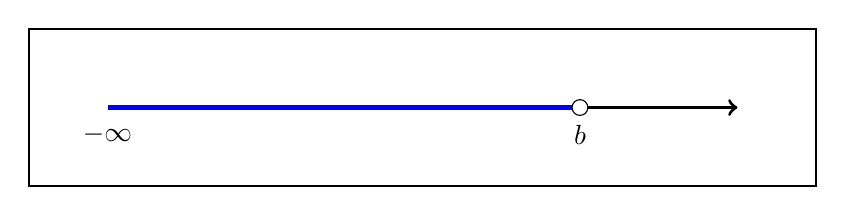
\begin{tikzpicture}
	    	\draw[thick] (-5, -1) rectangle (5, 1);
              % Eixo horizontal
              \draw[->, very thick] (-4,0) -- (4,0);
            
              % Linha vertical para representar x
              \draw[dashed] (2,-0.1) -- (2,0.1);
              % Rótulo para -∞
              \node[below] at (-4,-0.1) {$-\infty$};
              % Rótulo para x
              \node[below] at (2,-0.1) {$b$};
              % Desenhar o intervalo aberto (-∞, x)
              \draw[ultra thick, blue] (-4,0) -- (2,0);
              % Adicionar a bolinha aberta em x
              \draw[fill=white] (2,0) circle (0.1);
        \end{tikzpicture}
	}{
	    \Fonte{Elaborado pelo autor}
	}	
\end{figure}
Se tomarmos um $a \in \R$ fixo, com $a<b$, então a decomposição do intervalo $(-\infty, b)$ pode ser expressa por meio da união dos intervalos $(-\infty, a]$ e $(a,b)$, onde estão representados na figura a seguir pelas cores azul e vermelha, respectivamente.\\
\begin{figure}[h!]
	\centering
	\Caption{\label{fig:boreliano-decomposto} Representação de uma decomposição do intervalo $(-\infty, b)$ na reta real}	
	\UECEfig{}{
        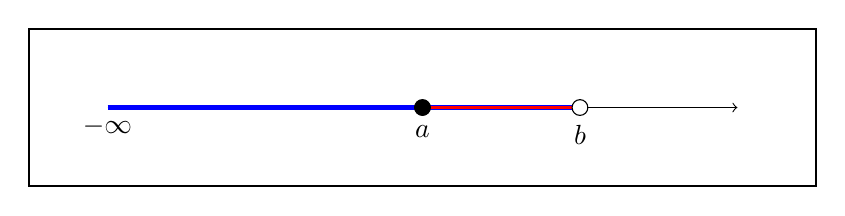
\begin{tikzpicture}
        	\draw[thick] (-5, -1) rectangle (5, 1);
              % Eixo horizontal
              \draw[->] (-4,0) -- (4,0);
              % Linha vertical para representar x
              \draw[dashed] (2,-0.1) -- (2,0.1);
              % Rótulo para -∞
              \node[below] at (-4,0) {$-\infty$};
              % Rótulo para x
              \node[below] at (2,-0.1) {$b$};
                
              % Rótulo para a
              \node[below] at (0,-0.1) {$a$};
              
              % Desenhar o intervalo aberto (-∞, x)
              \draw[ultra thick, blue] (-4,0) -- (2,0);
            
              % Desenhar o intervalo aberto (a,b)
              \draw[very thick, red] (0,0) -- (2,0);
              
              % Adicionar a bolinha aberta em x
              \draw[fill=white] (2,0) circle (0.1);
              \draw[fill=black] (0,0) circle (0.1);
        \end{tikzpicture}
	}{
	    \Fonte{Elaborado pelo autor}
	}	
\end{figure}\\
A decomposição de intervalos reais pela união de outros é relevante para mostrar a seguinte equivalência sobre a \sigal de Borel.\\
\begin{env}{Teorema}
\label{teo:equiv-borel}
    Uma \sigal é de Borel  se, e somente se, é gerada por intervalos do tipo $(a,b)$ com $a,b \in \R$.
    \vspace{-0.2cm}
\end{env}
\begin{prova}
   Suponha que $\borel$ seja a $\sigma$-álgebra de Borel. 
   Sejam $a$ e $b$ números reais, com $a<b$.
   Como $a + \dfrac{1}{n} \in \R$ para todo $n \in \N$, temos que o intervalo
   $
   \left(-\infty, a + \dfrac{1}{n}\right) \in \borel$ para todo $n \in \N
   $.
   Segue, pela \ref{prop:interseção-elementos-sigmas}, que
   $
   \displaystyle \bigcap_{n = 1}^\infty \left(-\infty, a+ \dfrac{1}{n}\right) \in \borel
   $.
   Com isso, afirmamos que a interseção de todos os intervalos $\left(-\infty, a + \dfrac{1}{n}\right)$ é igual ao intervalo $(-\infty, a]$.
   De fato,
   \begin{align*}
	x \in \bigcap_{n \in \N} \left(-\infty, a + \dfrac{1}{n}\right)
   	\Leftrightarrow & x \in \left(-\infty, a + \dfrac{1}{n}\right), \ \forall \ n \in \N\\
   	\Leftrightarrow & x < a + \dfrac{1}{n}, \ \forall \ n \in \N\\
   	\Leftrightarrow & \dlim_{n \to +\infty} x \leq \dlim_{n \to +\infty} \left(a + \dfrac{1}{n}\right)\\
   	\Leftrightarrow & x \leq a\\
   	\Leftrightarrow & x \in (-\infty, a].
   \end{align*}
	Logo, $(-\infty, a] \in \borel$ acarretando que $(a, +\infty) = (-\infty, a]^c \in \borel$.
	Observe que podemos decompor $(-\infty, b) = (-\infty,a] \cup (a, b)$ enquanto que $(a, +\infty) = (a, b) \cup [b, +\infty)$.
	Desta forma, vemos que $(-\infty, b) \cap (a, +\infty) = (a,b)$. 
	Como $(-\infty, b)$ e $(a, +\infty)$ são elementos de $\borel$, segue pela 
	\ref{prop:interseção-elementos-sigmas} que $(a,b) \in \borel$.
	Com isso, $\borel$ pode ser gerada por intervalos do tipo $(a,b)$ com $a,b \in \R$.
   
	Suponha, reciprocamente, que $\mathcal{C}$ é uma \sigal de $\R$ gerada por $(a,b)$ com $a,b \in \R$.
	Como $(a, b) \in \cc$, então $(a,b)^c \in \cc$, por definição de $\sigma$-álgebra.
	Logo, $(-\infty,a])\cup [b,+\infty) \in \cc$.
	Além disso, os conjuntos $A_n = (-n, a)$ são todos elementos de $\mathcal{C}$ para qualquer $n \in \N$.
	Segue, pela  \ref{def:sigma-algebra}, que 
	$\displaystyle \bigcup_{n = 1}^\infty (-n,a) \in \mathcal{C}$.
	Só que $\displaystyle \bigcup_{n = 1}^\infty (-n,a) = (-\infty, a)$. 
	Disso, $(-\infty, a)\cap \left\{(\infty,a])\cup [b,+\infty)\right\} \in \cc$. Portanto,  $(-\infty, a) \in \cc$ como queríamos.
	%% FFALTA PROVAR AINDA DIREITINHO.
\end{prova}

\section{Funções Mensuráveis}
Agora que já estamos familiarizados com os conceitos de \sigal e espaços mensuráveis, vamos aplicar, sobre este espaço uma função e estudar seu comportamento.
Iniciaremos tratando de funções reais e estenderemos o conceito conforme haja necessidade.
A partir de agora fixemos que, quando não houver menção contrária, $X$ será um conjunto qualquer diferente de $\varnothing$ e $\mathcal{C}$ será uma \sigal desse conjunto. 

\begin{env}{Definição}
	\label{def:mensurabilidade-funções-reais}
    Uma função $f: X \to \R $ é dita $\mathcal{C}$-mensurável se, para cada $\alpha \in \R$, o conjunto $\{x \in X;\ f(x) > \alpha\} \in \mathcal{C}$.
    \vspace{-0.2cm}
    \index{Função! $\cc$-mensurável}
\end{env}
% Exemplos de Funções mensuráveis
\begin{env}{Exemplo}
\label{ex:funcao-constante}
	Seja $K \in \R$ um número fixado. 
	A função constante $f: X \to \R$ definida por $f(x) = K$, para todo $x \in X$ é $\cc$-mensurável.
	\index{Função! constante}
	\vspace{-0.2cm}
\end{env}

Para mostrarmos este fato, precisamos analisar os casos de $\alpha$.
Assim
	\begin{enumerate}[label*= (\Roman*)]
		\item Se $\alpha \geq K$, então o conjunto $\{x \in X; f(x) > \alpha\} = \varnothing$ uma vez que não existe $x \in X$ tal que $f(x)= K > \alpha$.
		\item Se $\alpha < K$, então para todo $x \in X$, $f(x) > \alpha$.
		Logo, o conjunto $\{x \in X; f(x) > \alpha\} = X$.
	\end{enumerate}
Em todo caso, para todo $\alpha \in \R$, o conjunto  $\{x \in X;\ f(x) > \alpha\} \in \mathcal{C}$.
Portanto, a função constante $f$ é $\cc$-mensurável.
\begin{env}{Exemplo}
    Seja $(X, \mathcal{C})$ uma espaço mensurável e $A \in \mathcal{C}$.
    A função característica \index{Função! característica}\footnote{As vezes também é chamada  função indicadora.} de $A$ 
    $\chi_A: X \to \{0,1\}$ definida por 
    $$\chi_A(x) =\left\{\begin{array}{cc}
         1, & \textrm{\ se \ } x \in A \\
         0, & \textrm{\ se \ } x \notin A
    \end{array}\right.
    $$
    é $\cc$-mensurável.
    \vspace{-0.2cm}
\end{env}

Para verificar se $X_A$ é $\cc$-mensurável precisamos, novamente, analisar os casos de $\alpha \in \R$.
	\begin{enumerate}[label*= (\Roman*)]
		\item Se $\alpha \geq 1$, observamos que $\{x \in X; \chi_A(x)>  \alpha\} = \varnothing$, pois não há $x \in X$ tal que $\chi_A(x) > 1$.  
		\item Se $ 0 \leq \alpha < 1$, então o conjunto $\{x \in X; \chi_A(x)>  \alpha\} = A$, pois apenas valores $x \in A$ tem suas imagens $\chi_A(x) = 1$ e consequentemente $\chi_A(x) \geq \alpha$.
		\item  se $\alpha < 0$, podemos notar que o conjunto $\{x \in X; \chi_A(x)>  \alpha\} = X$, pois para qualquer que seja $x \in X$, os valores $\chi_A(x) \geq 0$.
	\end{enumerate}
Em todo o caso, vemos que o conjunto $\{x \in X; \chi_A(x)>  \alpha\}$ é um elemento de $\mathcal{C}$, pois $\varnothing, X$ e $A$ são elementos de $\mathcal{C}$. Portanto, a função característica $\chi_A(x)$ é $\cc$-mensurável.

\begin{env}{Proposição}
	\label{prop: propriedades de função característica}
	Dado um conjunto $X$, sejam $A, B \subset X$.
	Então $\chi_{A\cup B} = \chi_A + \chi_B - \chi_{A \cap B}$.
	Em particular, se $A \cap B = \varnothing$, então $\chi_{A\cup B} = \chi_A + \chi_B$
	\footnote{Esta proposição é um exercício que pode ser encontrado em \cite[p.57]{elon}.}.
\end{env}
\begin{prova}
	\hspace{-2.1cm}Perceba que 
	$\chi_{A^c} = 1 - \chi_A$ e que 
	$\chi_{A\cap B} = \chi_A\cdot \chi_B$.
	Logo, 
	\begin{equation}
		\chi_{A\cup B} = 1 - \chi_{(A\cup B)^c}
		= 1 - \chi_{A^c\cap B^c}
		= 1 - \chi_{A^c}\chi_{B^c}
		= 1 - (1-\chi_{A})(1-\chi_B)
	\end{equation}
	Daí, por meio da propriedade distributiva, 
	\begin{equation}
		1 - (1-\chi_{A})(1-\chi_B)
		=
		1 - (1 -\chi_{A} - \chi_{B} - \chi_{A}\chi_{B})
		=
		\chi_{A} + \chi_{B} + \chi_{A}\chi_{B}
		=
		\chi_{A} + \chi_{B} + \chi_{A\cap B}
	\end{equation}
	Combinando as equações (1) e (2) concluímos que 
	$
	\chi_{A\cup B}
	=
	\chi_{A} + \chi_{B} + \chi_{A\cap B}
	$
	
	\end{prova}
	\begin{env}{Exemplo}
	\label{ex:função-continua-mensuravel}
	    Considere o espaço mensurável $(\R, \borel)$. 
	    Toda função $f: \R \to \R$ contínua
	    \footnote{
	    	Lembre que \enquote{Uma função $f : X \to \R$ diz-se contínua no ponto $a \in X$ quando é possível tornar 
	    	$f(x)$ arbitrariamente próximo de $f(a)$ desde que
	    	se tome $x$ suficientemente próximo de $a$} \cite[p.222]{elon}.
    		Quando a função é contínua em todo ponto, dizemos apenas que ela é contínua.
    	}
     		 é Borel mensurável.
	    \index{Função! contínua}
	    \vspace{-0.2cm}
	\end{env}
	
		Para mostrar a validade do exemplo acima, precisamos de resultados auxiliares que serão enunciados a seguir sem demonstração para que o texto não descentralize do tema.
		\vspace{-0.2cm}
	\begin{env}{Proposição}
	\label{cit:função-continua-mensuravel}
		Suponha que $f:X \to \R$ seja contínua em todos os pontos de $X$.
		Se $X \subset \R$ é um aberto 
		%
		\footnote{\enquote{Um subconjunto $A \subset \R$ chama-se um \textit{conjunto aberto} quando
			todos os seus pontos são interiores [...] \cite[p.164]{elon}.}}, 
		%
		então o conjunto $A = \{a \in X;\ f(a)>k\}$ é um aberto \cite[p.226]{elon}.
		\vspace{-0.2cm}
		\index{Conjunto! aberto}
	\end{env}
	\begin{env}{Teorema}
		\label{teo:estrutura-abertos-reta}
		Todo subconjunto aberto $A \subset R$ se exprime, de modo único, como um reunião enumerável de intervalos abertos dois a dois disjuntos \cite[p.167]{elon}.
		\vspace{-0.2cm}
	\end{env}

	Segue disso que
	$\{x \in \R; f(x) > \alpha\} = \displaystyle \bigcup_{j = 1}^\infty A_j$ onde cada $A_j$ é um intervalo aberto, ou seja, $A_j \in \borel$ para todo $j \in \N$.
	Com isso, pela \ref{def:sigma-algebra}, o conjunto $\{x \in \R; f(x) > \alpha\} \in \borel$.
	Portanto, qualquer função contínua $f: \R \to \R$ é Borel mensurável.
    Lembre que ao apresentarmos a $\sigma$-álgebra de Borel (\ref{def:algebra-borel}), mostramos no \ref{teo:equiv-borel} que há mais de uma maneira de definir os borelianos.
    Para uma função $f: X \to \R$ $\cc$-mensurável, também podemos definir uma função $\cc$-mensurável por meio de conjuntos diferentes conforme exposto no seguinte teorema:
\begin{env}{Teorema}
\label{teo:equiv-funcoes-mensuraveis}
    Sendo $(X,\mathcal{C})$ um espaço mensurável, para uma função $f: X \to \R$ $\cc$-mensurável qualquer as seguintes afirmações são equivalentes:
    \vspace{-0.4cm}
    \begin{multicols}{2}    	
	    \begin{enumerate}[label=(\alph*)]
	        \item $\forall \ \alpha \in \R, \ A_\alpha =\{x \in X;\ f(x) > \alpha \} \in \mathcal{C}$;
	        \item $\forall \ \alpha \in \R, \ B_\alpha =\{x \in X;\ f(x) \leq \alpha \} \in \mathcal{C}$;
	        \item $\forall \ \alpha \in \R, \ C_\alpha =\{x \in X;\ f(x) \geq \alpha \} \in \mathcal{C}$;
	        \item $\forall \ \alpha \in \R, \ D_\alpha =\{x \in X;\ f(x) < \alpha \} \in \mathcal{C}$.
	    \end{enumerate}
     \end{multicols}
	\vspace{-0.2cm}
\end{env}
\begin{prova}
    Dividiremos esta demonstração em três partes. A estratégia será mostrar que a afirmação $(a)$ é equivalente à afirmação $(b)$; depois que a afirmação $(c)$ é equivalente à afirmação $(d)$ ; e por fim que a firmação $(a)$ ocorre se, e somente se, a afirmação $(c)$ ocorre. 
    \begin{enumerate}[label* = (\Roman*)]
        \item Suponha a validade da afirmação $(a)$. 
        Disso, $A_\alpha \in \cc \Leftrightarrow A_\alpha^c \in \cc$, pela definição de $\sigma$-álgebra.
	    Perceba que 
	    $$
	    x \in A_\alpha^c 
	    \Leftrightarrow
	    x \notin A_\alpha
	    \Leftrightarrow  
	    x \in X \textrm{\ e \ } f(x) \leq \alpha
	    \Leftrightarrow 
	    x \in B_\alpha    
		$$ 
		Assim, um elemento está em $A_\alpha^c$ se, e somente se, está em $B_\alpha$. Segue que $A_\alpha^c = B_\alpha$ e daí, $A_\alpha$ é um elemento de $\cc \Leftrightarrow B_\alpha$ é elemento de $\cc$.
		\item Para mostrar a equivalência entre as afirmações $(c)$ e $(d)$ utilizamos um argumento totalmente análogo à parte $(I)$, pois se $x \notin C_\alpha$, então $f(x) < \alpha$ acarretando que $x \in D_\alpha$ e vice-versa.
		\item Suponha que $A_\alpha \in \mathcal{C}$. Tome a sequência $\left(A_{\alpha -\frac{1}{n}}\right)$. Claramente, cada $A_{\alpha - \frac{1}{n}}$ é um elemento de $\mathcal{C}$ por definição.
		Logo, pela \ref{prop:interseção-elementos-sigmas}, a interseção $\displaystyle \bigcap_{n = 1}^\infty A_{\alpha -\frac{1}{n}} \in \mathcal{C}$.
		Além disso, note que 
		\begin{equation}
			x \in \displaystyle \bigcap_{n = 1}^\infty A_{\alpha -\frac{1}{n}}
			\Leftrightarrow
		 	x \in A_{\alpha - \frac{1}{n}}, \forall \ n \in \N
			\Leftrightarrow
			f(x)> \alpha -\dfrac{1}{n},  \ \forall \ n \in \N
		\end{equation}
		Como cada $f(x) \in \R$, temos que
		\begin{equation}
			\lim_{n \to \infty} f(x) \geq \lim_{n \to \infty} \left(\alpha - \dfrac{1}{n}\right)
			\Leftrightarrow
			f(x) \geq \alpha
			\Leftrightarrow
			x \in C_\alpha
		\end{equation}
		Segue das equivalências (1) e (2) que $C_\alpha = \displaystyle \bigcap_{n = 1}^\infty A_{\alpha -\frac{1}{n}} $.
		Portanto $C_\alpha \in \mathcal{C}$ como queríamos.
   \end{enumerate}
	
		Reciprocamente, suponha que $C_\alpha \in \mathcal{C}$. Tomemos a sequência $\left(C_{\alpha + \frac{1}{n}}\right)$.
		Cada elemento $C_{\alpha +\frac{1}{n}} \in \mathcal{C}$ por definição.
		Assim, pela definição de \sigal, 
		$\displaystyle \bigcup_{n = 1}^\infty C_{\alpha +\frac{1}{n}} \in \mathcal{C}$. Com isso, temos que
		\begin{align*}
		    x \in \displaystyle \bigcup_{n = 1}^\infty C_{\alpha +\frac{1}{n}}
		    \Leftrightarrow & x \in C_{\alpha + \frac{1}{n_0}}, \textrm{\ para algum  $n_0 \in \N$ }\\
		    \Leftrightarrow & f(x)\geq \alpha +\dfrac{1}{n_0}\\
		    \Leftrightarrow & f(x) > \alpha \\
		    \Leftrightarrow & x \in A_\alpha
		\end{align*}
		Assim, $\displaystyle \bigcup_{n = 1}^\infty C_{\alpha +\frac{1}{n}} = A_\alpha$. Logo, $A_\alpha \in \mathcal{C}$.
		Portanto, concluímos de $(I), (II)$ e $(III)$ que as afirmações $(a), (b), (c)$ e $(d)$ são todas equivalentes.
\end{prova}

% Aritmética de Funções mensuráveis
Perceba que mesmo na presença do \ref{teo:equiv-funcoes-mensuraveis}, mostrar que uma função é mensurável é trabalhoso e repetitivo uma vez que, geralmente, é preciso verificar os casos de $\alpha$.
Com o intuito de otimizar a identificação de uma função mensurável, veremos o comportamento de operações aritméticas entre funções mensuráveis.
%
\begin{env}{Proposição}
\label{prop:aritmetica-uma-funcao}
Seja $f: X \to \R$ uma função real $\cc$-mensurável e $c \in \R$. Então as funções $cf$, $f^2$ e $|f|$ são $\cc$-mensuráveis. 
\vspace{-0.2cm}
\end{env}
\begin{prova}
	\vspace{-0.8cm}
    \begin{enumerate}[label*=(\alph*)]
        \item Mostraremos que $cf$ é $\cc$-mensurável para todos os casos possíveis do número real $c \in \R$.
            \begin{enumerate}[label=(\roman*)]
                \item Se $c = 0$, então $c\cdot f(x) = 0, \ \forall \ x \in X$, ou seja, $cf$ se torna a função constante. Segue pelo  \ref{ex:funcao-constante} que $cf$ é $\cc$-mensurável.
                
                \item Se $c>0$, então  dado $\alpha \in \R$, temos $cf(x) > \alpha \Leftrightarrow f(x) >\dfrac{\alpha}{c}$. 
                Logo, 
                $$
                \{x \in X; cf(x) > \alpha\} 
                = 
                \left\{x \in X; f(x) > \dfrac{\alpha}{c}\right\}
                $$
                    
                Isso ocorre para todo $\alpha$ e $f$ é $\cc$-mensurável, isto é, $\left\{x \in X; f(x) > \dfrac{\alpha}{c}\right\} \in \mathcal{C}$  . Logo, $cf$ é $\cc$-mensurável.
                
                \item Por fim, se $c < 0$, então existe um $ 0 < z \in \R$ tal que $c = -z$.
                Assim, 
                $$cf(x) >\alpha \Leftrightarrow -zf(x) >\alpha \Leftrightarrow f(x) < -\dfrac{\alpha}{z}$$
                Assim, o conjunto $\{x \in X; cf(x) > \alpha \} = \left\{x \in X; f(x) < -\dfrac{\alpha}{z}\right\}$.
                Desta forma, o conjunto  $\left\{x \in X; f(x) < -\dfrac{\alpha}{z}\right\}  \in \mathcal{C}$ pelo  item $(d)$ do  \ref{teo:equiv-funcoes-mensuraveis}. Portanto,  $cf$ é $\cc$-mensurável em todos os casos de $c \in \R$.
            \end{enumerate}
        %  
        \item Para mostrar a mensurabilidade de $f^2$ é também necessário analisar os casos de $\alpha$.
            \begin{enumerate}[label = (\roman*)]
                \item Se $\alpha < 0$, então $\{x \in X; [f(x)]^2 > \alpha\} = X$, pois $[f(x)]^2 \geq 0$ para todo $x \in X$.
                
                \item Se $\alpha \geq 0$, então para todo $x \in X$ $[f(x)]^2 > \alpha \Leftrightarrow f(x) > \sqrt{\alpha}$ ou $f(x) < -\sqrt{\alpha}$.
                Assim, um elemento 
                $x_0 \in \{x \in X; [f(x)]^2 > \alpha\}$ se, e somente se, $x_0 \in \{x \in X; f(x)> \sqrt{\alpha}\}$ ou \linebreak $x_0 \in \{x \in X; f(x)< -\sqrt{\alpha}\}$.
                Com isso, 
                \vspace{-0.4cm}
                $$\left\{x \in X; [f(x)]^2 > \alpha\right\} = \left\{x \in X; f(x)> \sqrt{\alpha}\right\}\cup \left\{x \in X; f(x)< -\sqrt{\alpha}\right\}.$$
                
                \vspace{-0.4cm}
                Como $f$ é $\cc$-mensurável por hipótese, temos que $\{x \in X; f(x)> \sqrt{\alpha}\} \in \mathcal{C}$ e \linebreak $\{x \in X; f(x)< -\sqrt{\alpha}\} \in \mathcal{C}$.
                Desta forma, usando a definição de \sigal, obtemos que  $\{x \in X; f(x)> \sqrt{\alpha}\} \cup \{x \in X; f(x)< -\sqrt{\alpha}\} \in \mathcal{C}$. Consequentemente, 
                $\{x \in X; [f(x)]^2 > \alpha\} \in \mathcal{C}$ acarretando a mensurabilidade de $f^2$.
            \end{enumerate}
        %
        \item Analogamente ao item anterior, se $\alpha < 0$, $\{x \in X; |f(x)| > \alpha\} = X$.
        Por outro lado, se $\alpha \geq 0$, vemos que 
        $\{x \in X; |f(x)| > \alpha\}=\{x \in X; f(x)> \alpha\} \cup \{x \in X; f(x)< -\alpha\}$.
        Assim, a mensurabilidade de $f$ acarreta na mensurabilidade de $|f|$ como desejávamos.
    \end{enumerate}
\end{prova}

% Exemplo de funções mensuráveis com aritmética
Antes de provarmos a próxima proposição, vamos enunciar um teorema que nos auxiliará na próxima demonstração. 
\begin{env}{Lema}
	\label{lem:densidade de Q em R}
	O conjunto $\Q$ dos números racionais e o conjunto
	$\R - \Q$ dos números irracionais são ambos densos
	\footnote{
		\enquote{Um conjunto $X \subset \R$ chama-se denso em $\R$ quando todo
			intervalo aberto $(a, b)$ contém algum ponto de $X$}\cite[p.83]{elon}.}
	 em $\R$ \cite[p.84]{elon}.
\end{env}

A prova do \ref{lem:densidade de Q em R} será omitida para que o texto não prolongue-se mais do que o necessário.
\begin{env}{Proposição}
\label{prop:aritmetica-duas-funcoes}
    Sejam $f,g:X \to \R$. Se $f$ e $g$ são ambas $\cc$-mensuráveis, então as funções $f+g$ e $f\cdot g$ são também $\cc$-mensuráveis.
    \vspace{-0.2cm}
\end{env}
\begin{prova}
    Provaremos, primeiramente, que $f+g$ é $\cc$-mensurável.
    Ora, por hipótese, $f$ e $g$ são $\cc$-mensuráveis. 
    Assim, dado $r \in \Q$, os conjuntos $\{x \in X; f(x) > r\}$ e 
    $\{x \in X; g(x) > \alpha -r\}$ são ambos elementos de $\mathcal{C}$.
    Considere o conjunto  
    \vspace{-0.2cm}
    $$H_r = \{x \in X; f(x) > r\} \cap \{x \in X;\ g(x) > \alpha -r\}$$
    
    \vspace{-0.2cm}
    Isto é, o conjunto dos elementos $x \in X$ tal que $f(x) 
    > r$ e $g(x) >\alpha -r$ simultaneamente.
    Assim, afirmamos que $\{x \in X; (f+g)(x) > \alpha\} = \displaystyle \bigcup_{r \in \Q} H_r$. Com efeito, tomemos um elemento 
    $a \in \{x \in X; (f+g)(x) > \alpha\}$.
    Assim, 
    $$
    (f+g)(a) > \alpha 
    \Rightarrow 
    f(a) + g(a) > \alpha 
    \Rightarrow f(a) > \alpha - g(a). 
    $$
    Agora, por densidade, tome um racional $r_0 \in \Q$ tal que  $f(a) > r_0 >\alpha - g(a)$, de forma que $f(a) > r_0$ e $g(a) > \alpha - r_0.$
    Logo, $a \in H_{r_0}$.
    Portanto, $ \displaystyle a \in \bigcup_{r \in \Q} H_r$.
    
    Reciprocamente, sendo $ \displaystyle a \in \bigcup_{r \in \Q} H_r$ existe um elemento $r_0 \in \Q$ tal que $a \in H_{r_0}$.
    Logo, $f(a) > r_0$ e $g(a) > \alpha -r_0$.
    Ao somarmos membro à membro temos
    \vspace{-0.2cm}
    $$
    f(a) + g(a) > r_0 + \alpha -r_0
    \Rightarrow
    (f + g)(a) > \alpha. 
    \vspace{-0.2cm}
    $$
    Com isso, $a \in \{x \in X; (f +g)(x) > \alpha\}$ como queríamos.
    Concluindo que a afirmação é verdadeira. 
    
    Além disso, para cada $r \in \Q$, o conjunto $H_r$ é um elemento de $\mathcal{C}$, pois é  a interseção de dois elementos de $\mathcal{C}$ ( \ref{prop:interseção-elementos-sigmas}).
    Note também que, pela definição de $\mathcal{C}$, a coleção $\displaystyle \bigcup_{r \in \Q} H_r$ é um elemento de $\mathcal{C}$, pois $\Q$ é enumerável.
    Segue que $f+g$ é $\cc$-mensurável.

    Para mostrar que $fg$ é mensurável basta notar que é a combinação de outras funções $\cc$-mensuráveis.
    De fato, dado $x \in X$, temos
    	\vspace{-0.2cm}
	    \begin{align*}
	        4(fg)(x) 
	        =& \ 2(fg)(x) +  2(fg)(x)\\
	        =& \ [f(x)]^2 - [f(x)]^2 + 2f(x)g(x) + [g(x)]^2 - [g(x)]^2 + 2f(x)g(x)\\
	        =& \ \left([f(x)]^2 + 2f(x)g(x) + [g(x)]^2\right)  - \left([g(x)]^2 - 2f(x)g(x) + [f(x)]^2\right)\\
	        =& \ (f(x) +g(x))^2 - (f(x) - g(x))^2\\
	        =& \ [(f+g)(x)]^2 - [(f-g)(x)]^2.    
    	\end{align*}
    \vspace{-0.2cm}
    Logo, $fg = \dfrac{1}{4}\left[(f+g)^2 - (f-g)^2\right]$.
    Sendo $g$ mensurável, podemos usar a \ref{prop:aritmetica-uma-funcao} pondo $c= -1$.
    Assim, temos $(-1)g = -g$ acarretando que $-g$ é mensurável.
    Além disso, pela parte \textit{(a)} desta proposição, $f - g = f+ (-g)$ é mensurável.
    Segue que $fg$ é $\cc$-mensurável
    \footnote{A \ref{prop:aritmetica-uma-funcao} e \ref{prop:aritmetica-duas-funcoes} encontram-se enunciadas na forma de um único lema em \cite[p.9]{bartle}}.
\end{prova}
\begin{env}{Definição}
	\label{def:parte-positiva e negativa}
    Seja $f: X \to \R$ uma função real. 
    Dizemos que a \textbf{parte positiva} da função $f$ é a função $f^+: X \to \R$ definida por $f^+(x) = \max\{f(x), 0\}$
    \index{Parte! positiva}
    %
    \footnote{A notação $\sup X$ indica o supremo do conjunto $X$. 
    	Segundo \citeauthor{elon}, \enquote{Sejam $K$ um corpo ordenado e $X \subset K$ um subconjunto limitado superiormente. 
    	Um elemento $b \in K$ chama-se \textit{supremo} do
    	subconjunto $X$ quando $b$ é a menor das cotas superiores de $X$ em $K$} \cite[p.75]{elon}.  
	}.
	%
    Semelhantemente, chamamos de a \textbf{parte negativa} da função $f$, a função $f^-: X \to \R$ definida por $f^-(x) = \max\{-f(x), 0\}$ \index{Parte! negativa}.
\vspace{-0.2cm}\end{env}

É possível  que a definição de parte positiva e negativa de funções fique um pouco abstrata em um primeiro contato. 
Numa tentativa de esclarecer ao máximo, daremos o seguinte exemplo:
\begin{env}{Exemplo}
	\label{ex:parte-positiva e negativa}
    Seja $f: \R^* \to \R$ definida por $f(x) =\dfrac{|x|}{x}$, ou seja, 
    $f(x) = \left\{
    \begin{array}{ll}
    1,& \text{se\ } x > 0\\
    -1,& \text{se\ } x < 0\\	
    \end{array}\right. 
    $.
    Assim sua parte positiva e negativa são, respectivamente:
    \begin{center}
	    $f^+(x) = \left\{
	    \begin{array}{ll}
	    	1,& \text{se\ } x > 0\\
	    	0,& \text{se\ } x < 0\\	
	    \end{array}\right. 
	    $
	    e
	    $f^-(x) = \left\{
	    \begin{array}{ll}
	    	0,& \text{se\ } x > 0\\
	    	1,& \text{se\ } x < 0\\	
	    \end{array}\right. 
	    $	
    \end{center}
    
\vspace{-0.2cm}\end{env}

Com isso, a figura \ref{fig: Gráfico da Função f(x) =|x|/x} apresenta o gráfico da função $f$ do \ref{ex:parte-positiva e negativa} ao passo que as figuras \ref{fig: GrafPartPosFunção f(x) =|x|/x} e \ref{fig: GrafPartNegFunção f(x) =|x|/x} representam os gráficos das partes positiva e negativa de $f$, respectivamente.

    \begin{figure}[h!]
	\centering
	\Caption{\label{fig: Gráfico da Função f(x) =|x|/x} Gráfico da Função $f(x) =\dfrac{|x|}{x}$}	
	\UECEfig{}{
	    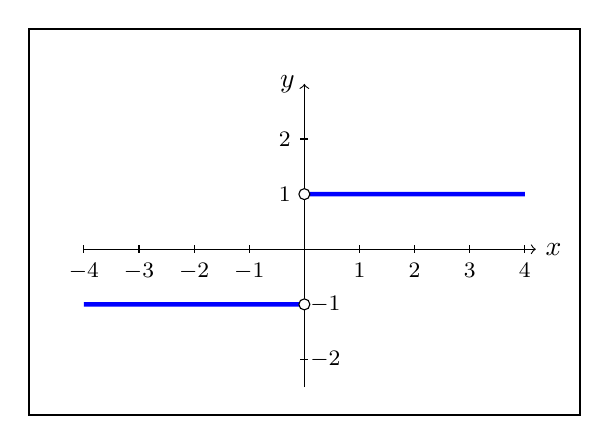
\begin{tikzpicture}[scale=0.7]
	    	% Retangulo em volta
	    	\draw[thick] (-5, -3) rectangle (5, 4);
	    	% Eixos
	    	\draw[->] (-4,0) -- (4.2,0) node[right] {$x$};
	    	\draw[->] (0,-2.5) -- (0, 3) node[left] {$y$};
	    	% Rótulos
	    	\foreach \i in {-4,-3,-2,-1,1,2,3,4}{
	    		\draw (\i,2pt)--(\i, -2pt) node[below]{{\footnotesize $\i$}};
	    	}
	    	\foreach \i in {1,2}{
	    		\draw (2pt,\i)--(-2pt,\i) node[left]{{\footnotesize $\i$}};
	    	}
            \foreach \i in {-2,-1}{
            	\draw (2pt,\i)--(-2pt,\i) node[right]{{\footnotesize $\i$}};
            }    
            \draw[domain=-4:-0.1,ultra thick,variable=\x,blue] plot ({\x},{abs(\x)/\x});
            \draw[domain=0.1:4,ultra thick,variable=\x,blue] plot ({\x},{abs(\x)/\x});
        
            \draw[fill=white] (0,1) circle (0.1);
            \draw[fill=white] (0,-1) circle (0.1);
        
            \end{tikzpicture}
	}{
	    \Fonte{Elaborado pelo autor}
	}	
    \end{figure}    
	\begin{figure}[h!]
		\centering
		\Caption{\label{fig: GrafPartPosFunção f(x) =|x|/x} Gráfico da parte positiva da função $f(x) =\dfrac{|x|}{x}$}	
		\UECEfig{}{
			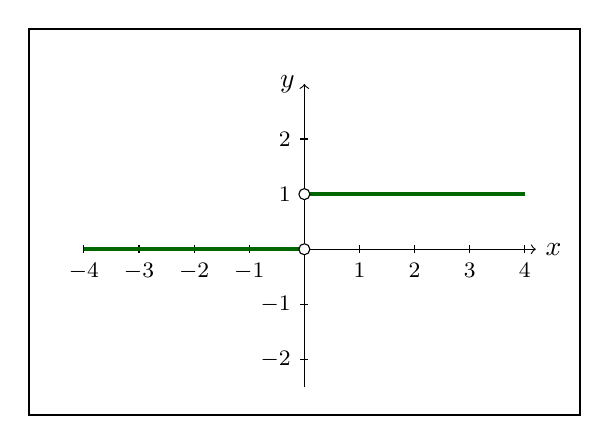
\begin{tikzpicture}[scale=0.7]
				% Retangulo em volta
				\draw[thick] (-5, -3) rectangle (5, 4);
				% Eixos
				\draw[->] (-4,0) -- (4.2,0) node[right] {$x$};
				\draw[->] (0,-2.5) -- (0, 3) node[left] {$y$};
				% Rótulos
				\foreach \i in {-4,-3,-2,-1,1,2,3,4}{
					\draw (\i,2pt)--(\i, -2pt) node[below]{{\footnotesize $\i$}};
				}
				\foreach \i in {-2,-1,1,2}{
					\draw (2pt,\i)--(-2pt,\i) node[left]{{\footnotesize $\i$}};
				}
				
				\draw[domain=-4:-0.1,ultra thick,variable=\x,green!40!black] plot ({\x},{0});
				\draw[domain=0.1:4,ultra thick,variable=\x,green!40!black] plot ({\x},{1});
				
				\draw[fill=white] (0,1) circle (0.1);
				\draw[fill=white] (0,0) circle (0.1);
				
			\end{tikzpicture}
		}{
			\Fonte{Elaborado pelo autor}
		}	
	\end{figure}
\begin{figure}[h!]
	\centering
	\Caption{\label{fig: GrafPartNegFunção f(x) =|x|/x} Gráfico da parte negativa da função $f(x) =\dfrac{|x|}{x}$}
	\UECEfig{}{
		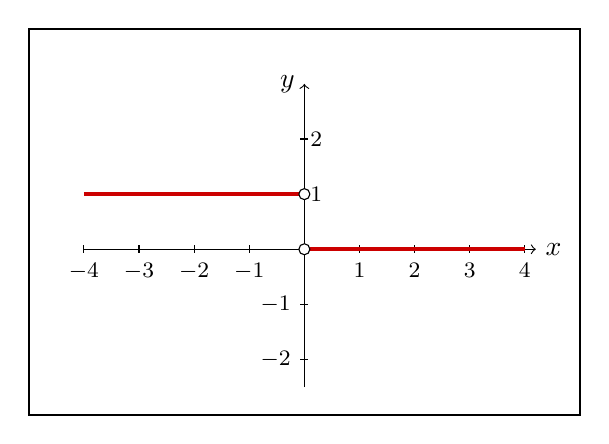
\begin{tikzpicture}[scale=0.7]
			% Retangulo em volta
			\draw[thick] (-5, -3) rectangle (5, 4);
			% Eixos
			\draw[->] (-4,0) -- (4.2,0) node[right] {$x$};
			\draw[->] (0,-2.5) -- (0, 3) node[left] {$y$};
			% Rótulos
			\foreach \i in {-4,-3,-2,-1,1,2,3,4}{
				\draw (\i,2pt)--(\i, -2pt) node[below]{{\footnotesize $\i$}};
			}
			\foreach \i in {1,2}{
				\draw (2pt,\i)--(-2pt,\i) node[right]{{\footnotesize $\i$}};
			}
			\foreach \i in {-2,-1}{
				\draw (2pt,\i)--(-2pt,\i) node[left]{{\footnotesize $\i$}};
			}
			\draw[domain=-4:-0.1,ultra thick,variable=\x,red!80!black] plot ({\x},{1});
			\draw[domain=0.1:4,ultra thick,variable=\x,red!80!black] plot ({\x},{0});
			
			\draw[fill=white] (0,1) circle (0.1);
			\draw[fill=white] (0,0) circle (0.1);
			
		\end{tikzpicture}
	}{
		\Fonte{Elaborado pelo autor}
	}	
\end{figure}

Para finalizarmos esta seção apresentaremos uma relação interessantes sobre uma função mensurável e suas partes positiva e negativa.

    \begin{env}{Lema}
    \label{lem:f = f^+ - f^-}
        Seja $f: X \to \R$ uma função real. Então $f = f^+ - f^-$ e $|f| = f^+ + f^-$.
    \end{env}
    \begin{prova}
            Para provar que $f = f^+ - f^-$, devemos avaliar os casos de $f(x)$. 
            Logo, se $f(x) \geq 0$, então $f^+(x) = \max\{f(x), 0\} = f(x)$ e $f^-(x) = \max\{-f(x), 0\} = 0$, pois $f(x) \geq 0$ implica  $- f(x) \leq~0$.
            Disso, $f^+(x) - f^-(x) = f(x) - 0 = f(x)$, ou seja, $(f^+ - f^-)(x) = f(x)$ tal que $f(x) \geq 0$.
            Caso $f(x) <~0$, então $- f(x) > 0$. 
            Com isso,  $\max\{f(x), 0\} = 0$ e $\max\{-f(x), 0\} = -f(x)$.
            Desta forma vemos que
            $f^+(x) - f^-(x) = 0 - (-f(x)) = f(x)$.
            Em todo caso, $f = f^+ - f^-$.
			Analogamente, se $f(x) \geq 0$, então  $\sup\{f(x), 0\} = f(x)$ e $\sup\{-f(x), 0\} = 0$.
            Assim, $f^+(x) + f^-(x) = f(x)$.
            Caso, $f(x) < 0$, então $ - f(x) > 0$.
            Com isso, obtemos $\sup\{f(x), 0\} = 0$ e $\sup\{-f(x), 0\} = -f(x)$.
            Logo, $f^+(x) + f^-(x) = -f(x)$.
            Desta forma, 
            $$
            (f^+ + f^-)(x) = \max\{f(x), -f(x)\} = |f(x)|.
            $$
            Portanto, $f^+ + f^- = |f|$.
    \end{prova}

Observe que o \ref{lem:f = f^+ - f^-} nos dá a forma das funções $f^+$ e $f^-$ de maneira implícita.
De fato, somando as duas expressões membro a membro vemos que
\vspace{-0.2cm}
$$f + |f| = (f^+ - f^-) + (f^+ + f^-) = 2f^+$$

\vspace{-0.2cm}
Assim, podemos expressar $f^+ = \dfrac{|f| + f}{2}$.
De modo semelhante, conseguimos subtrair membro a membro e obter a expressão $f^- = \dfrac{|f| - f}{2}$. 
Isso demonstra o lema adiante:
\begin{env}{Lema}
\label{lem:forma-explicita-partes-de-uma-funcao}
    Se $f: X \to \R$ é uma função real, então $f^+ = \dfrac{|f| + f}{2}$ e $f^- = \dfrac{|f| - f}{2}$.
    \vspace{-0.2cm}
\end{env}
\begin{env}{Teorema}
    Uma função $f: X \to \R$ é $\cc$-mensurável se, e somente se, suas partes negativa e positiva são ambas $\cc$-mensuráveis. 
    \vspace{-0.2cm}
\end{env}
    \begin{prova}
        Suponha que $f$ seja $\cc$-mensurável.
        Pela  \ref{prop:aritmetica-uma-funcao} vemos que a função $|f|$ é $\cc$-mensurável e pelo \ref{lem:forma-explicita-partes-de-uma-funcao} as funções $f^+ = \dfrac{1}{2}(|f| + f)$ e $f^- = \dfrac{1}{2}(|f| - f)$ também são $\cc$-mensuráveis.
        Reciprocamente, supondo que $f^+$ e $f^-$ são mensuráveis, temos pelo \ref{lem:f = f^+ - f^-} que
        $f = f^+ - f^-$. Segue, novamente pela \ref{prop:aritmetica-duas-funcoes}, que $f$ é $\cc$-mensurável. 
    \end{prova}

Nesta seção, vimos o conceito de $\sigma$-álgebra e, por meio dele, definimos a mensurabilidade de uma função bem como mostramos propriedades disso.
Todos esses conceitos e definições serviram para as seções expostas adiante. 
Na seção seguinte, exploraremos o conceito central deste trabalho: a teoria da medida.´ 
        \chapter{A Teoria da Medida}
%%%%%%%%% ESPAÇOS MENSURÁVEIS
    Nesta seção, apresentaremos o conceito chave desse trabalho: a teoria da medida.
    Conhecemos este conceito de forma intuitiva pelo o que vemos, geralmente, na geometria euclidiana plana.
    Aqui, trataremos de medida de modo generalizado. 
    Para isso, precisaremos ampliar o conjunto dos números reais para que ele possa atender novas exigências.
    Isso é necessário porquê, as vezes, teremos conjuntos tão \enquote{grandes} que nenhum número real poderá representar sua medida. 
    Assim, estenderemos o conjunto dos números reais na primeira seção.
    Na seguinte, estenderemos o conceito de função mensurável para o conjunto dos números reais estendidos e, na seção final, apresentaremos a definição de medida bem como exemplos dela.
\section{Os Espaços de Funções Mensuráveis}

    \begin{env}{Definição}
    \label{def:reta-estendida}
        A coleção $\xreta$ que consiste de $\R \cup \{-\infty, +\infty\}$ é chamada de \textbf{Sistema Estendido de Números Reais}.
        \vspace{-0.2cm}
    \end{env}

    Ou seja, $\xreta$ nada mais é que o conjunto dos números reais com a possibilidade de se ter $-\infty$ ou $+\infty$.
    Com isso, parece que nosso problema de medir conjuntos muito grandes se resolveu.
    Entretanto, alguns cuidados são necessários para operarmos em $\xreta$.
    Um deles, por exemplo, é que $\xreta$ não é fechado para operações de $\R$ tais como $(+\infty) + (-\infty)$ que nem definido é.
    Dito isso, para $x \in \R$, as operações dos símbolos $+\infty$ e $-\infty$ são dadas da seguinte forma:
    \vspace{-0.4cm}
    \begin{multicols}{2}
        \begin{itemize}
            \item $(+ \infty) + (+ \infty)  = + \infty$;
            \item $x + (+ \infty) = (+ \infty) + x = + \infty$;
            \item $(- \infty) + (- \infty)  = - \infty$;
            \item $x + (- \infty) = (- \infty) + x = - \infty$;
            \item $(+ \infty)\cdot (+ \infty) =  +\infty $;
            \item $(- \infty)\cdot (- \infty) =  +\infty $;
            \item $(+ \infty)\cdot (- \infty) =  -\infty $;
            \item $(- \infty)\cdot (+ \infty) =  -\infty $.
        \end{itemize}
    \end{multicols}
	
	\vspace{-0.4cm}
    Na multiplicação, dependendo do número real, a operação diferencia-se.
    Assim, podemos ter
    \vspace{-1cm}
    \begin{multicols}{2}
    $$
    x \cdot (+\infty) = (+\infty) \cdot x =
    \left\{\begin{array}{cc}
          +\infty, & \ \textrm{se } x > 0\\
          0, & \ \textrm{se } x = 0\\
          - \infty, & \textrm{se } x < 0
    \end{array}\right.
    $$
    
    $$
    x \cdot (-\infty) = (-\infty) \cdot x =
    \left\{\begin{array}{cc}
          -\infty, & \ \textrm{se } x > 0\\
          0, & \ \textrm{se } x = 0\\
          + \infty, & \textrm{se } x < 0
    \end{array}\right.
    $$  
    \end{multicols}
	\vspace{-0.4cm}
    Neste novo contexto de números reais a \sigal de Borel não é mais válida uma vez que a definição \ref{def:algebra-borel} não inclui $+\infty$ nem $-\infty$.
    Logo, precisaremos de uma $\sigma$-álgebra em $\xreta$ para dar continuidade aos nossos estudos. 
    Com isso, considere $\xreta$.
    Tomando um conjunto arbitrário $E \in \borel$, com $\varnothing \neq E$, defina $E_1 = E \cup \{-\infty\}, E_2 = E \cup \{+\infty\}$ e $E_3 = E \cup \{-\infty, +\infty\}$. 
    Desta forma, o conjunto $\overline{\borel} = \displaystyle \bigcup_{E \in \borel} \{E, E_1, E_2, E_3\}$ é uma \sigal de $\xreta$.
    \begin{comment}
    Com efeito, se $E \in \borel$, então é um intervalo aberto conforme o teorema \ref{teo:equiv-borel}.
    Assim, $E_1, E_2, E_3$ e $E_4$ serão intervalos do tipo $[-\infty,x)$ ou $(x, +\infty]$ que são elementos de $\borel$ acrescidos de $+\infty$ ou $-\infty$. 
    Deste modo, é fácil verificar que se um elemento $A \in \xborel$, então $A^c \in \xborel$.
    Além disso, a união enumerável é, no máximo, o intervalo $[-\infty,+\infty]$ que é exatamente $\xreta$.
    Desta forma, $\xborel$ é uma \sigal de $\xreta$.
    	
    \end{comment}
    
    \begin{env}{Definição}
    \label{def:algebra-borel-estendida}
        A \sigal $\overline{\borel} = \displaystyle \bigcup_{E \in \borel} \{E, E_1, E_2, E_3\}$ do conjunto $\xreta$ é chamada de Álgebra de Borel Estendida. 
        \vspace{-0.2cm}
    \end{env}

    Uma vez que estamos familiarizados com os conceitos de funções de valores reais mensuráveis, estamos prontos para estender este conceito para o conjunto $\xreta$.
    \begin{env}{Definição}
    \label{def:familia-funcoes-mensuraveis}
        Sendo $(X, \mathcal{C})$ um espaço mensurável, uma função de valores reais estendidos $f: X \to \xreta$ é dita $\mathcal{C}$-mensurável caso o conjunto
        $\{x \in X; f(x) > \alpha\} \in \mathcal{C}$ para qualquer que seja $\alpha \in \R$. 
        \vspace{-0.4cm}
    \end{env}

	Denotaremos a família de todas as funções de valores reais estendidos de $X$ que são $\mathcal{C}$-mensuráveis por $M(X, \mathcal{C})$.
	Além disso, caso estivermos tratando apenas das funções não negativas usaremos $M^+(X, \mathcal{C})$.
    \begin{env}{Proposição}
    \label{prop:identidade-intersecao-mais-infinito}
        Se $f \in \menfus$, então $\{x \in X; f(x) = +\infty\} = \displaystyle \bigcap_{n = 1}^\infty \{x \in X; f(x) > n\}$.
    \end{env}
    \begin{prova}
        Tome, de modo arbitrário, um elemento $a \in X$. 
        Assim, 
        \begin{align*}
            a \in \bigcap_{n = 1}^\infty \{x \in X; f(x) > n\} 
            \Leftrightarrow & a \in \{x \in X; f(x) > n\}, \ \forall n \in \N\\
            \Leftrightarrow & \forall\ n \in \N,\ f(a) > n\\
            \Leftrightarrow & f(a) = +\infty.  
        \end{align*}
    Além disso, note que cada $\{x \in X; f(x) > n\} \in \mathcal{C}$.
    Segue, pela \ref{prop:interseção-elementos-sigmas}, que \linebreak $\displaystyle \bigcap_{n = 1}^\infty \{x \in X; f(x) > n\} \in \mathcal{C}$ acarretando que $\{x \in X; f(x) = +\infty\} \in \mathcal{C}$. 
    \end{prova}

    \begin{env}{Proposição}
    \label{prop:identidade-união-menos-infinito}
        Se $f \in \menfus$, então $\{x \in X; f(x) = -\infty\} = \displaystyle \left(\bigcup_{n = 1}^\infty \{x \in X; f(x) > - n\}\right)^c$.
        \vspace{-0.4cm}
    \end{env}
	%
    \begin{prova}
    	
    	\vspace{-0.6cm}
        Analogamente à proposição \ref{prop:identidade-intersecao-mais-infinito} tomemos $a \in X$. 
        Segue que 
        \begin{align*}
            a \in \left(\bigcup_{n = 1}^\infty \{x \in X; f(x) > - n\}\right)^c
            \Leftrightarrow & \ a \in \bigcap_{n = 1}^\infty \left(\{x \in X; f(x) > - n\}\right)^c\\
            \Leftrightarrow & \forall \ n \in \N, a \in \left(\{x \in X; f(x) > - n\}\right)^c\\
            \Leftrightarrow & \forall \ n \in \N, a \notin \{x \in X; f(x) > - n\}\\
            \Leftrightarrow & \forall \ n \in \N, a \in \{x \in X; f(x) \leq - n\}\\    
            \Leftrightarrow & \forall \ n \in \N, f(a) \leq - n\\
            \Leftrightarrow & \lim_{n \to \infty} f(a) \leq \lim_{n \to \infty} (- n)\\  
            \Leftrightarrow & f(a) = -\infty.                  
        \end{align*}
    
    Com isso, podemos perceber que 
    $\displaystyle a \in \left(\bigcup_{n = 1}^\infty \{x \in X; f(x) > - n\}\right)^c \Leftrightarrow  a \in \{x \in X; f(x) = -\infty\}$.
    Ora, cada $\{x \in X; f(x) > - n\} \in \mathcal{C}$.
    Assim, por definição de \sigal, temos que $ \displaystyle\bigcup_{n = 1}^\infty \{x \in X; f(x) > - n\} \in \mathcal{C}$ e também 
    $\displaystyle\left(\bigcup_{n = 1}^\infty \{x \in X; f(x) > - n\}\right)^c \in \mathcal{C}$.
    Concluímos disso que $\{x \in X; f(x) = -\infty\} \in \mathcal{C}$ como queríamos provar. 
    \end{prova}
    \begin{env}{Teorema}
    \label{teo:condição-de-mensurabilidade}
        Uma função de valores reais estendidos $f: X \to \xreta$ é $\cc$-mensurável se, e somente se, os conjuntos 
        $A = \{ x \in X; f(x) = +\infty\}$ e $B = \{x \in X; f(x) = -\infty\}$
		 são elementos de $\mathcal{C}$ e a função $h: X \to \R$ definida por
		 \vspace{-0.2cm}
		 $$
		 h(x) = \left\{\begin{array}{cc}
		     f(x), & \textrm{\ se } x \notin A\cup B  \\
		      0,& \textrm{\ se } x \in A\cup B
		 \end{array}\right.
	 	 \vspace{-0.2cm}
		 $$
		 é $\cc$-mensurável.
		 \vspace{-0.2cm}
	 \end{env}
\begin{prova}
    Suponha que $f \in \menfus$. 
    Logo, pela \ref{prop:identidade-intersecao-mais-infinito} e \ref{prop:identidade-união-menos-infinito}, os conjuntos $A$ e $B$ são elementos de $\mathcal{C}$.
    Assim, tome $\alpha \in \R$ com $\alpha \geq 0$, então os elementos de $\{x \in X; h(x) > \alpha\}$ são os elementos de $\{x \in X; f(x) > \alpha\}$ que não estão em $A$, pois $h$ tem contradomínio $\R$.
    Como $\cc$ é uma \sigal\hspace{-0.1cm}, $A \in \cc \Rightarrow A^c \in \cc$. 
    Com isso, 
    \vspace{-0.2cm}
    $$
    \{x \in X; h(x) > \alpha\} = A^c\cap \{x \in X; f(x) > \alpha\} \in \cc
    \vspace{-0.2cm}
    $$
    Segue, pela  \ref{prop:interseção-elementos-sigmas} que $\{x \in X; h(x) > \alpha\} \in \cc$, ou seja, $h$ é $\cc$-mensurável.
    Caso, $\alpha < 0$, então $\{x \in X; h(x) > \alpha\} = \{x \in  X ; f(x) > \alpha\} \cup B $, pois $h(x) = 0$ para $x \in A \cup B$.
    Desta forma $h$ é $\cc$-mensurável.

    Por outro lado, se supormos que $A$ e $B$ são elementos de $\mathcal{C}$ e $h$ é $\cc$-mensurável, então
    $$\{x \in X; f(x) > \alpha\} = \{x \in  X ; h(x) > \alpha\} \cup A $$
    quando $\alpha \geq 0$, e 
    $$\{x \in X; f(x) > \alpha\} = \{x \in  X ; h(x) > \alpha\} \cap B^c $$
    quando  $\alpha < 0$, por motivos análogos à primeira parte da demonstração.
    Portanto, $f$ é uma função $\cc$-mensurável como desejávamos.
\end{prova}

Como consequência do \ref{prop:aritmetica-uma-funcao} e o \ref{teo:condição-de-mensurabilidade} obtemos, imediatamente, que se $ f \in M(X,\mathcal{C})$, então as funções $cf, f^2, |f|, f^+$ e $f^-$ também são elementos de $M(X, \mathcal{C})$.
Entretanto, um resultado análogo à \ref{prop:aritmetica-duas-funcoes} não é possível em $\xreta$.
Isso acontece porquê em $\xreta$ a operação de adição não é bem definida.
Então caso $f(x) = +\infty$ e $g(x) = -\infty$ para algum $x \in \R$ a adição
$f(x) + g(x)$ não é realizada.
Por outro lado, a função $fg$ é $\cc$-mensurável se $f$ e $g$ forem ambas $\cc$-mensuráveis.
Para mostrar isso, precisamos de alguns resultados que serão expostos adiante

\begin{env}{Teorema}
\label{teo:mensurabilidade-sequencia-funcoes-mensuraveis}
	Seja $(f_n)$ uma sequência de elementos de $\menfus$ e defina as funções
	$$f(x) = \inf f_n(x),\  
	F(x) = \sup f_n(x),\  
	f^*(x) = \lim\inf f_n(x),\   
	F^*(x) = \lim\sup f_n(x).$$
	Então as funções $f, f^*, F$ e $F^*$ são elementos de $\menfus$.
\end{env}
\begin{prova}
	Como $(f_n)$ é uma sequência de funções $\cc$-mensuráveis e $f = \inf f_n$, afirmamos que $\{x \in X; f(x) \geq \alpha\} = \displaystyle \bigcap_{n = 1}^\infty \{x \in X; f_n(x) \geq \alpha\}$.
	De fato, tomemos um elemento $y \in X$.
	Assim, 
		\begin{align*}
			y \in \bigcap_{n = 1}^\infty \{x \in X; f_n(x) \geq \alpha\} \Leftrightarrow	&
			y \in \{x \in X; f_n(x) \geq \alpha\}\ \forall\  n \in \N\\
			\Leftrightarrow	&	
			f_n(y) \geq \alpha\ \forall \ n \in \N\\
			\Leftrightarrow	&	
			\inf_{n \in \N}f_n(y) \geq \inf_{n \in \N}\alpha\ \forall \ n \in \N\\
			\Leftrightarrow	&	
			f(y) \geq \alpha\ \forall\  n \in \N\\
			\Leftrightarrow	&
			y \in \{x \in X; f(x) \geq \alpha\}
		\end{align*}
	Como cada $\{x \in X; f_n(x) \geq \alpha\}$ é $\cc$-mensurável, segue pela proposição \ref{prop:interseção-elementos-sigmas} que o conjunto $\{x \in X; f(x) \geq \alpha\} \in \cc$ para todo $\alpha \in \R$.
	Desta forma, $f$ é $\cc$-mensurável.
	
	Observe, também, que $\{x \in X; F(x) >\alpha\} = \displaystyle \bigcup_{n = 1}^\infty \{x \in X; f_(x) >\alpha\}$.
	Com efeito, para $y \in X$ 
	\begin{align*}
		y \in \bigcup_{n = 1}^\infty \{x \in X; f_n(x) > \alpha\} \Leftrightarrow	&
		\ \exists\ k \in \N \textrm{tal que\ } y \in \{x \in X; f_k(x) > \alpha\}\\
		\Leftrightarrow	&	
		f_k(y) > \alpha\\
		\Leftrightarrow	&	
		F(x) \geq f_k(y) > \alpha\\
		\Leftrightarrow	&	
		F(x) > \alpha,\ \forall \alpha \in \R\\
		\Leftrightarrow	&
		y \in \{x \in X; F(x) > \alpha\}
	\end{align*}
	Assim, concluímos que $f$ e $F$ são $\cc$-mensuráveis. 
	Note que a mensurabilidade de $f^*$ e $F^*$ vem de $f$ e $F$ uma vez que
	$$
	f^*(x) = \sup_{n \geq 1} \left\{\inf_{m \geq n} f_m(x)\right\}
	\textrm{\ e\ }
	F^*(x) = \inf_{n \geq 1} \left\{\sup_{m \geq n} f_m(x)\right\}
	$$
\end{prova}
\begin{env}{Corolário}
	\label{cor:convergencia-de-uma-sequencia-mensuravel}
	Se $(f_n)$ é uma sequência em $\menfus$ que converge para $f$ em $X$, então
	$f$ também está em $\menfus$.
	\vspace{-0.2cm}
\end{env}
\begin{prova}
	Ora, por hipótese $\displaystyle f(x) = \lim_{n \to +\infty} f_n(x)$.
	Só que $\displaystyle \lim_{n \to +\infty} f_n(x) = \lim_{n \in \N} \inf f_n(x)$.
	Segue que $\displaystyle f(x) = \lim_{n \in \N} \inf f_n(x)$ que, por sua vez, é $\cc$-mensurável pelo teorema anterior.
\end{prova}

% Parte final do Capítulo - Truncamento
\begin{env}{Definição}
	Seja $f$ uma função em $\menfus$ e $A > 0$.
	Definimos o truncamento $f_A$ da função $f$ por
	$$ f_A(x) =
	\left\{\begin{array}{cc}
		f(x), & \textrm{se\ } |f(x)| \leq A \\
		A, & \textrm{se\ } f(x) > A \\
		-A, & \textrm{se\ } f(x) < -A 
	\end{array}\right.
	\vspace{-0.4cm}
	$$
\end{env}
\begin{env}{Proposição}
	\label{prop:truncamento-mensurável}
	Seja $A$ um número real maior que zero.
	Se $f$ é uma função em $\menfus$, então $f_A$ é uma função $\cc$-mensurável.
\end{env}
\begin{prova}
	Basta provar que para qualquer que seja $\alpha \in \R$, tem-se $\{x \in X; f_A(x) > \alpha\} \in \cc$.
	Para isso, vamos analisar os casos de $\alpha$.
	Se $-A \leq \alpha \leq A$, então $f_A(x) = f(x)$ para todo $x \in X$.
	Logo, 
	$$
	\{x \in X; f_A(x) > \alpha \} = \{x \in X; f(x) > \alpha \}
	$$
	Como $f$ é mensurável, $\{x \in X; f(x) > \alpha \} \in \cc$.
	Caso $\alpha > A$, então
	$$
	\{x \in X; f_A(x) > \alpha \} = \varnothing \in \cc.
	$$
	Pois, por definição de $f_A$, não existe valor maior que $A$.
	Caso tenhamos $\alpha < -A$, ocorre que
	$$
	\{x \in X; f_A(x) > \alpha \} = X \in \cc.
	$$
	Pois todos os valores que $f_A$ assume são maiores ou igual à $-A$.
	Em todo caso, o conjunto $\{x \in X; f_A(x) > \alpha\}$ é um elemento de $\cc$.
	Portanto, $f_A$ é $\cc$-mensurável. 
\end{prova}
% Exemplos de Truncamento

\begin{comment}

\begin{env}{Exemplo}
	Seja $f \in \menfus$ tal que $f(x) = x^2-2$.
	Então o truncamento $f_2$ é representado, graficamente, como
	\begin{figure}[h!]
		\centering
		\Caption{\label{fig:representação do truncamento da função} representação do truncamento $f_2$ da função $f(x) = x^2-2$} 
		\UECEfig{}{
			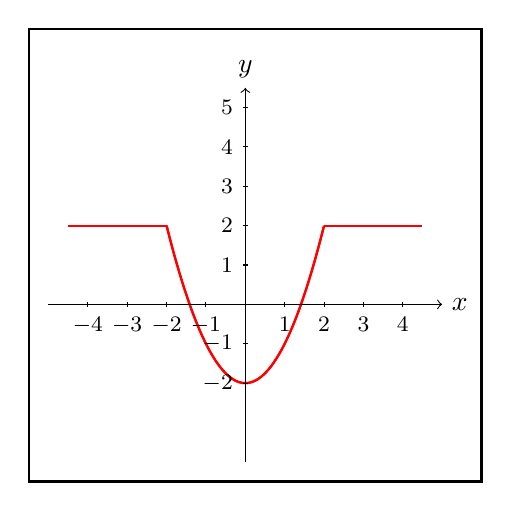
\begin{tikzpicture}[scale=0.5]
				\draw[thick] (-5.5, -4.5) rectangle (6, 7);
				% Defina o intervalo x
				\def\xmin{-3}
				\def\xmax{3}
%				
%				% Desenhe a função f(x)
%				\draw[domain=\xmin+0.4:\xmax-0.4, smooth, samples=100, blue] plot (\x, {\x*\x -2});
				
				% Desenhando a função f_2
				\draw[domain=2:4.5, thick, samples=100, red] plot (\x, {2});
				\draw[domain=-4.5:-2, thick, samples=100, red] plot (\x, {2});
				\draw[domain=-2:2, thick, samples=100, red] plot (\x, {\x*\x -2});
				\draw[domain=-2:2, thick, samples=100, red] plot (\x, {\x*\x -2});
				% Adicione rótulos aos eixos
				\draw[->] (\xmin-2,0) -- (\xmax+2,0) node[right] {$x$};
				\draw[->] (0,\xmin-1) -- (0,\xmax+2.5) node[above] {$y$};
				
                % Rótulos
				\foreach \i in {-4,-3,-2,-1,1,2,3,4}{
					\draw (\i,2pt)--(\i, -2pt) node[below]{{\footnotesize $\i$}};
				}
				
				\foreach \i in {-2, -1, 1,2,3,4,5}{
					\draw (2pt,\i)--(-2pt, \i) node[left]{{\footnotesize $\i$}};
				}
			\end{tikzpicture}
		}{
			\Fonte{Elaborado pelo autor}		}   
	\end{figure}
	
\end{env}
\end{comment}
Para que possamos entender melhor o truncamento de uma função, apresentamos o seguinte exemplo:
\pagebreak
\begin{env}{Exemplo}
	Seja $g \in \menfus$ tal que $g(x) = 3\cos(2x)$.
\end{env}
	\begin{figure}[h!]
		\centering
		\Caption{\label{fig:3cosseno_de_2x} Gráfico da função $g(x) = 3\cos (2x)$} 
		\UECEfig{}{
			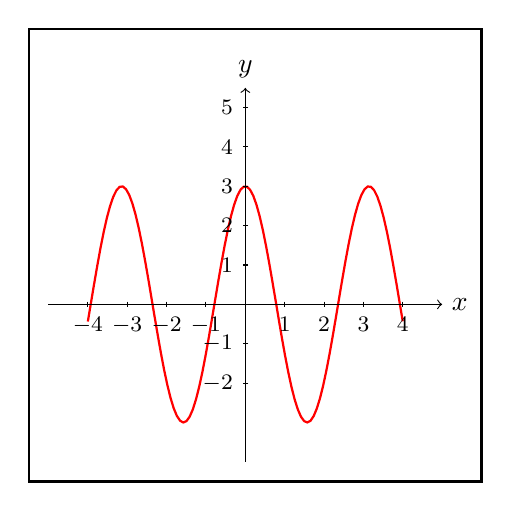
\begin{tikzpicture}[scale=0.5]
				\draw[thick] (-5.5, -4.5) rectangle (6, 7);
				% Defina o intervalo x
				\def\xmin{-3}
				\def\xmax{3}
				%				
				%				% Desenhe a função f(x)
				%				\draw[domain=\xmin+0.4:\xmax-0.4, smooth, samples=100, blue] plot (\x, {\x*\x -2});
				
				% Desenhando a função f_2
				\draw[domain=-4:4, thick, samples=100, red] plot (\x, {3*cos(2*\x r)});
				% Adicione rótulos aos eixos
				\draw[->] (\xmin-2,0) -- (\xmax+2,0) node[right] {$x$};
				\draw[->] (0,\xmin-1) -- (0,\xmax+2.5) node[above] {$y$};
				
				% Rótulos
				\foreach \i in {-4,-3,-2,-1,1,2,3,4}{
					\draw (\i,2pt)--(\i, -2pt) node[below]{{\footnotesize $\i$}};
				}
				
				\foreach \i in {-2, -1, 1,2,3,4,5}{
					\draw (2pt,\i)--(-2pt, \i) node[left]{{\footnotesize $\i$}};
				}
			\end{tikzpicture}
		}{
			\Fonte{Elaborado pelo autor}		}   
	\end{figure}

	Uma truncamento faz, didaticamente falando, uma espécie de limitação no gráfico da função original.
	Ao tomarmos como constante o número real 1, vemos que o truncamento $g_1$ da função $g$, apresentada anteriormente, \enquote{amassa} o gráfico de $g$ nas ordenadas 1 e $-1$ como exposto na figura \ref{fig:truncamentog_1}.
		\begin{figure}[h!]
			\centering
			\Caption{\label{fig:truncamentog_1} Gráfico do truncamento $g_1$ } 
			\UECEfig{}{
				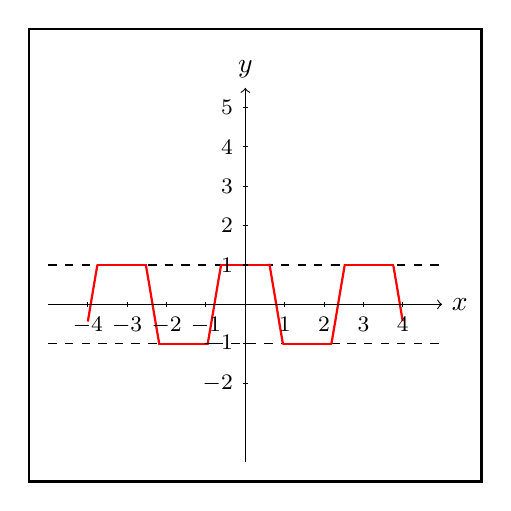
\begin{tikzpicture}[scale=0.5]
					\draw[thick] (-5.5, -4.5) rectangle (6, 7);
					% Defina o intervalo x
					\def\xmin{-3}
					\def\xmax{3}
					%				
					%				% Desenhe a função f(x)
					%				\draw[domain=\xmin+0.4:\xmax-0.4, smooth, samples=100, blue] plot (\x, {\x*\x -2});
					
					% Desenhando a função f_2
					%\draw[domain=-4:4, thick, samples=100, red] plot (\x, {3*cos(2*\x r)});
					\draw[domain=-5:5, dashed, samples=100] plot (\x, {1});
					\draw[domain=-5:5, dashed, samples=100] plot (\x, {-1});
					
					\draw[domain=-4:-3.755, thick, samples=100, red] plot (\x, {3*cos(2*\x r)});
					\draw[domain=-3.76:-2.55, thick, samples=100, red] plot (\x, {1});
					\draw[domain=-2.53:-2.18, thick, samples=100, red] plot (\x, {3*cos(2*\x r)});
					\draw[domain=-2.19:-0.96, thick, samples=100, red] plot (\x, {-1});
					\draw[domain=-0.96:-0.61, thick, samples=100, red] plot (\x, {3*cos(2*\x r)});
					\draw[domain=-0.61:0.635, thick, samples=100, red] plot (\x, {1});
					\draw[domain=0.61:0.96, thick, samples=100, red] plot (\x, {3*cos(2*\x r)});
					\draw[domain=0.96:2.19, thick, samples=100, red] plot (\x, {-1});
					\draw[domain=2.185:2.53, thick, samples=100, red] plot (\x, {3*cos(2*\x r)});
					\draw[domain=2.53:3.76, thick, samples=100, red] plot (\x, {1});]
					\draw[domain=3.76:4, thick, samples=100, red] plot (\x, {3*cos(2*\x r)});
					% Adicione rótulos aos eixos
					\draw[->] (\xmin-2,0) -- (\xmax+2,0) node[right] {$x$};
					\draw[->] (0,\xmin-1) -- (0,\xmax+2.5) node[above] {$y$};
					
					% Rótulos
					\foreach \i in {-4,-3,-2,-1,1,2,3,4}{
						\draw (\i,2pt)--(\i, -2pt) node[below]{{\footnotesize $\i$}};
					}
					
					\foreach \i in {-2, -1, 1,2,3,4,5}{
						\draw (2pt,\i)--(-2pt, \i) node[left]{{\footnotesize $\i$}};
					}
				\end{tikzpicture}
			}{
				\Fonte{Elaborado pelo autor}		}   
		\end{figure}	
	
Note que o mesmo ocorre com o truncamento $g_2$ apresentado na figura \ref{fig:truncamentog_2} onde, desta vez, $g$ é limitada pelas ordenadas $2$ e $-2$.
		\begin{figure}[h!]
			\centering
			\Caption{\label{fig:truncamentog_2} Gráfico do truncamento $g_2$ } 
			\UECEfig{}{
				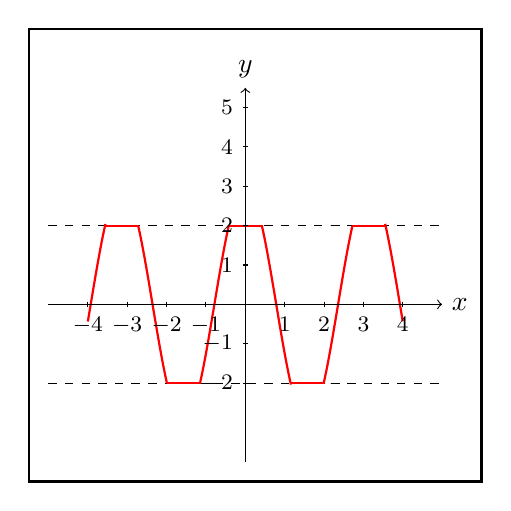
\begin{tikzpicture}[scale=0.5]
					\draw[thick] (-5.5, -4.5) rectangle (6, 7);
					% Defina o intervalo x
					\def\xmin{-3}
					\def\xmax{3}
					%				
					%				% Desenhe a função f(x)
					%				\draw[domain=\xmin+0.4:\xmax-0.4, smooth, samples=100, blue] plot (\x, {\x*\x -2});
					
					% Desenhando a função f_2
					%\draw[domain=-4:4, thick, samples=100, red] plot (\x, {3*cos(2*\x r)});
					\draw[domain=-5:5, dashed, samples=100] plot (\x, {2});
					\draw[domain=-5:5, dashed, samples=100] plot (\x, {-2});
					
					\draw[domain=-4:-3.552, thick, samples=100, red] plot (\x, {3*cos(2*\x r)});
					\draw[domain=-3.55:-2.71, thick, samples=100, red] plot (\x, {2});
					\draw[domain=-2.72:-1.99, thick, samples=100, red] plot (\x, {3*cos(2*\x r)});
					\draw[domain=-2:-1.15, thick, samples=100, red] plot (\x, {-2});
					\draw[domain=-1.15:-0.42, thick, samples=100, red] plot (\x, {3*cos(2*\x r)});
					\draw[domain=-0.43:0.43, thick, samples=100, red] plot (\x, {2});
					\draw[domain=0.42:1.16, thick, samples=100, red] plot (\x, {3*cos(2*\x r)});
					\draw[domain=1.15:2, thick, samples=100, red] plot (\x, {-2});
					\draw[domain=1.99:2.72, thick, samples=100, red] plot (\x, {3*cos(2*\x r)});
					\draw[domain=2.72:3.55, thick, samples=100, red] plot (\x, {2});]
					\draw[domain=3.552:4, thick, samples=100, red] plot (\x, {3*cos(2*\x r)});
					% Adicione rótulos aos eixos
					\draw[->] (\xmin-2,0) -- (\xmax+2,0) node[right] {$x$};
					\draw[->] (0,\xmin-1) -- (0,\xmax+2.5) node[above] {$y$};
					
					% Rótulos
					\foreach \i in {-4,-3,-2,-1,1,2,3,4}{
						\draw (\i,2pt)--(\i, -2pt) node[below]{{\footnotesize $\i$}};
					}
					
					\foreach \i in {-2, -1, 1,2,3,4,5}{
						\draw (2pt,\i)--(-2pt, \i) node[left]{{\footnotesize $\i$}};
					}
				\end{tikzpicture}
			}{
				\Fonte{Elaborado pelo autor}		}   
		\end{figure}
Assim, quanto maior o número $n$ do truncamento $g_n$ de uma função mensurável $g$, mais próximo $g_n$ está de $g$ uma vez que a \enquote{limitação} vai desaparecendo.

Com essas observações podemos voltar a analisar o produto de duas funções com valores reais estendidos.
Considere $f,g \in \menfus$. 
Tomemos duas sequências $(f_n)$ e $(g_m)$ tais que para cada $k \in \N$, $f_k$ e $g_k$ são truncamentos de $f$ e $g$, respectivamente.
Ou seja,
	\hspace{-0.2cm}
	\begin{minipage}{0.5\linewidth}
	$$ g_k(x) =
	\left\{\begin{array}{cc}
		g(x), & \textrm{se\ } |g(x)| \leq k \\
		k, & \textrm{se\ } g(x) > k \\
		-k, & \textrm{se\ } g(x) < k 
	\end{array}\right.	
	$$	
	\end{minipage}
e
	\begin{minipage}{0.5\linewidth}
		$$ f_k(x) =
		\left\{\begin{array}{cc}
			f(x), & \textrm{se\ } |f(x)| \leq k \\
			k, & \textrm{se\ } f(x) > k \\
			-k, & \textrm{se\ } f(x) < k 
		\end{array}\right.	
		$$	
	\end{minipage}
\\

Para qualquer que seja o valor de $k \in \N$.
Pela \ref{prop:truncamento-mensurável}, $f_k$ e $g_p$ são $\cc$-mensuráveis para cada $k$ e $p$ números naturais.
Assim, pela \ref{prop:aritmetica-duas-funcoes}, $f_kg_p$ também é $\cc$-mensurável para quaisquer $k, p \in \N$.
Como mencionado anteriormente, o truncamento de uma função $f$ causa uma \enquote{limitação} em sua imagem.
Logo, se tomarmos $n$ grande o suficiente, o truncamento $f_n$ da função $f$ tende a se aproximar da própria função $f$.
Desta forma, fixemos um $m \in \N$.
Assim, para $x \in X$
$$
\lim_{k \to +\infty} \left(f_k(x)g_m(x)\right) = f(x)g_m(x) 
$$
Segue pelo \ref{cor:convergencia-de-uma-sequencia-mensuravel} que 
$fg_m \in \menfus$. 
Analogamente, para $x \in X$
$$
\lim_{m \to +\infty} \left(f(x)g_m(x)\right) 
= f(x)g(x) = (fg)(x)
$$
Concluímos, pelo mesmo corolário, que $fg \in \menfus$.
Dito isso, encerraremos esta seção apresentando a definição generalizada de mensurabilidade de uma função.

\begin{env}{Definição}
	\label{def:mensurabilidade-geral}
	Sejam $(X, \cc)$ e $(Y,\mathcal{F})$ dois espaços mensuráveis.
	Dizemos que uma função $\phi:X \to Y$ é dita mensurável se o conjunto $f^{-1}(E) = \{x \in X; f(x)\in E\} \in \cc$ para todo conjunto $E \in \mathcal{F}$. 
\end{env}

Embora essa definição pareça ser totalmente distinta da \ref{def:mensurabilidade-funções-reais}, as duas são equivalentes no caso particular de $Y = \R$ e $\mathcal{F} = \borel$ conforme demonstrado a seguir.

\begin{env}{Proposição}
	Seja $(X, \cc)$ um espaço mensurável e $f$ uma função.
	Então $f$ é $\cc$-mensurável se, e somente se, $f^{-1}(E) \in \cc$ para todo boreliano $E$. 
\end{env}
\begin{prova}
	Suponha $f$ uma função $\cc$-mensurável. 
	Sabemos pela definição \ref{def:algebra-borel} que os elementos da álgebra de Borel são do tipo $(-\infty,x)$ com $x \in \R$.
	Assim, dado arbitrariamente $\alpha \in \R$ temos que
	$$
	f^{-1}(-\infty, \alpha)
	=\{x \in X; f(x) \in (-\infty, \alpha)\}
	=\{x \in X; f(x) \leq \alpha\}
	%\footnote{$f^{-1}(-\infty, \alpha)$ indica a pré imagem de $(-\infty, \alpha)$.}
	$$
	Como $f$ é $\cc$-mensurável segue pelo teorema \ref{teo:equiv-funcoes-mensuraveis} que $f^{-1}(-\infty, \alpha) \in \cc$.
	Reciprocamente se 
	$f^{-1}(-\infty, \alpha) \in \cc$ para qualquer $\alpha$ concluímos, imediatamente, que $\{x \in X; f(x) < \alpha\} \in \cc$ para todo $\alpha \in \R$.
	Portanto, $f$ é $\cc$-mensurável.
\end{prova}
%%%%%%%%%% Espaços de Medida

\section{Espaços de Medida}
Antes de definimos uma medida, lembraremos de alguns conceitos e resultados da teoria de conjuntos que nos serão úteis adiante.

\begin{env}{Definição}
\label{def:sequência-crescente-decrescente-de-conjuntos}
    Uma sequência de conjuntos $(A_n)$ é dita \textbf{não-decrescente} se $A_n \subseteq A_{n+1}$ para todo $n \in \N$.
    Caso tenhamos $A_n \supseteq A_{n+1}$ para todo $n \in \N$, dizemos que a sequência  de conjuntos é \textbf{não-crescente}.
\end{env}

\begin{env}{Proposição}
\label{prop:sequencia-crescente-conjuntos-resultado-A_n}
Seja $(E_n)$ uma sequência crescente de conjuntos. Se $(A_n)$ é tal que $A_1 = E_1$ e $A_n = E_n - E_{n -1}$ para todo $n > 1$, então:
\begin{enumerate}[label* = (\roman*)]
    \item $A_n$ é uma sequência disjunta;
        \footnote{Lembre que uma sequência disjunta significa que $A_i \cap A_j = \varnothing$ para todo $i \neq j$}
    \item $E_n = \displaystyle \bigcup_{j = 1}^n A_j$;
    \item $\displaystyle \bigcup_{j = 1}^\infty E_n = \displaystyle \bigcup_{j = 1}^\infty A_n$;
\end{enumerate}
\end{env}

\begin{prova}
    Para provar $(a)$ precisamos mostrar que para todo $n,m \in \N$ se $m \neq n$, então $A_n \cap A_m = \varnothing$.
    Suponha, sem perder generalidade, que $n > m > 1$.
    Assim, pela comutatividade e associatividade da relação de interseção e união de conjuntos segue que
    \begin{align*}
        A_m\cap A_n =& (E_m - E_{m -1}) \cap (E_n - E_{n -1})\\
        =& (E_m \cap E_{m -1}^c) \cap (E_n \cap E_{n -1}^c)\\
        =& (E_m \cap E_n) \cap ( E_{m -1}^c\cap E_{n -1}^c)\\
        =& (E_m \cap E_n) \cap \left( E_{m -1}\cup E_{n -1}\right)^c
    \end{align*}
	Como $(E_n)$ é não-decrescente, segue que $E_m \subseteq E_n$ e $E_{m-1}\subseteq E_{n-1}$.
    Deste modo, 
    $$
    (E_m \cap E_n) \cap \left( E_{m -1}\cup E_{n -1}\right)^c
    =
    E_m \cap E_{m-1}^c
    = \varnothing.
    $$
	Pois, se $x$ não é elemento de $E_{m-1}$ e $E_{m-1} \subseteq E_m$, então $x$ não pode ser elemento de $E_m$.
    
    Provaremos agora o item $(b)$.
 	Se $m = 1$, então não há o que fazer.
 	Suponha $m > 1$.
 	Assim, 
 	\begin{align*}
 		\bigcup_{j = 1}^m A_j
 		=&
 		\bigcup_{j = 1}^m(E_j\cap E_{j-1}^c)\\
 		=&
 		E_1 \cup (E_2\cap E_{1}^c) \cup (E_3\cap E_{2}^c) \cup \cdots
 		\cup (E_m\cap E_{m-1}^c)\\
 		=&
 		\left[(E_1 \cup E_2)\cap (E_1\cup E_{1}^c)\right]
 		\cup
 		\left[(E_2 \cup E_3)\cap (E_2\cup E_{2}^c)\right]
 		\cup
 		\cdots
 		\cup 
 		\left[(E_{m-1} \cup E_m)\cap (E_{m-1}\cup E_{m-1}^c)\right]\\
 		=&
 		\left[(E_1 \cup E_2)\cap X\right]
 		\cup
 		\left[(E_2 \cup E_3)\cap X\right]
 		\cup
 		\cdots
 		\cup 
 		\left[(E_{m-1} \cup E_m)\cap X\right]\\
 		=&
 		(E_1 \cup E_2)
 		\cup
 		(E_2 \cup E_3)
 		\cup
 		\cdots
 		\cup 
 		(E_{m-1} \cup E_m)\\
 		=&
 		E_1 \cup E_2 \cup E_3\cup 
 		\cdots
 		\cup E_{m-1} \cup E_m\\
 		=& E_m.
 	\end{align*}
	A última igualdade ocorre pelo fato de $(E_n)$ ser não-decrescente.
	Assim, $E_1 \subseteq E_2 \subseteq \cdots \subseteq E_m$.
	
    Por fim, $(c)$ é um resultado imediato, pois $ x \in \displaystyle \bigcup_{j = 1}^\infty E_j$ se, e somente se, 
    existe um $n_0 \in \N$ tal que $x \in E_{n_0}$. 
    Pelo item $(b)$, isso só ocorre se $x \in \displaystyle \bigcup_{j = 1}^{n_0}A_j$.
    Mas isso é equivalente à dizer que existe um $k$ com $1\leq k\leq n_0$ tal que $x \in A_k$.
    Como $k \in \N$ isso acontece se, e somente se, $x \in A_k$ para algum $k \in \N$.
    Portanto $x \in \displaystyle \bigcup_{j = 1}^\infty A_j$.
\end{prova}

\begin{env}{Proposição}
\label{prop:sequencia-decrescente-conjuntos-resultado-A_n}
Seja $(F_n)$ uma sequência não-crescente de conjuntos. 
Se $(E_n)$ é tal que $E_n = F_1 - F_n$ para todo $n \in \N$, então $(E_n)$ é não-decrescente e 
$\displaystyle \bigcup_{j = 1}^\infty E_n = \displaystyle F_1 - \bigcup_{j = 1}^\infty F_n$.
\end{env}

\begin{prova}
    Queremos mostrar que $(E_n)$ é não-decrescente, isto é, $E_n \subseteq E_{n+1}$ para todo $n \in \N$.
    Dado um $n \in \N$, tome $x \in E_n$. 
    Logo, $x \in F_1$ e $x \notin F_n$, por construção.
    Como $(F_n)$ é não-crescente, ocorre $F_{n} \supseteq F_{n+1}$. 
    Assim, $x \notin F_n \Rightarrow x \notin F_{n+1}$.
    Com isso, $x \in F_1$ e $x \notin F_{n+1}$, ou seja,
    $x \in E_{n+1}$.
    Desta maneira, $E_n \subseteq E_{n+1}$ para qualquer $n \in \N$ como queríamos.
    Além disso, um elemento $y \in \displaystyle \bigcup_{n \in \N} E_n$ se, e somente se,
    $y \in \displaystyle \bigcup_{n \in \N} (F_1 - F_n)$.
    Isso é equivalente a dizer que existe um $n_0 \in \N$ tal que $y \in F_1 - F_{n_0}$.
    Correspondentemente, $ y \in F_1$ e $y \notin F_{n_0}$ para algum $n_0 \in \N$.
    Isso ocorre se, e somente se, $y \in F_1$ e $y \notin \displaystyle \bigcup_{n \in \N} F_n$.
    Portanto, $\displaystyle \bigcup_{j = 1}^\infty E_n = \displaystyle F_1 - \bigcup_{j = 1}^\infty F_n$.
\end{prova}

\begin{env}{Proposição}
	\label{prop: duas partições}
	Se $\displaystyle \bigcup_{j = 1}^n E_j$ e $\displaystyle \bigcup_{k = 1}^m F_k$ são duas partições distintas de um conjunto $X$, então
	para cada $j \in I_n$ tem-se $E_j = \displaystyle \bigcup_{k = 1}^n (E_j \cap F_k)$.
\end{env}
\begin{prova}
	Fixemos um $j_0 \in I_n$.
	Assim, temos que $x \in \bigcup_{k = 1} (E_{j_0} \cap F_k)$ implica que existe um $k_0 \in I_m$ tal que  $x \in E_{j_0}\cap F_{k_0}$.
	Logo, $x \in E_{j_0}$ e $x \in F_{k_0}$, isto é, $x \in E_{j_0}$.
	Reciprocamente, se $y \in X$, então para algum $j_1 \in I_n$, $y \in E_{j_1}$, pois $\{E_j\}$ formam uma partição de $X$.
	Como $\{F_k\}$ também é uma partição de $X$, deve existir um $k_1 \in I_m$ tal que $x \in F_{k_1}$.
	Assim, $x \in E_{j_1} \cap F_{k_1}$. 
	Desta forma, existe um $k_1 \in I_m$ tal que $x \in \displaystyle \bigcup_{k = 1} (E_{j_1} \cap F_{k_1})$ como queríamos.	 
\end{prova}

\begin{env}{Definição}
\label{def:medida}
    Uma medida é uma função $\mu: (X, \mathcal{C}) \to \xreta$ tal que satisfaz as seguintes condições:
    \begin{enumerate}[label* = (\roman*)]
        \item $\mu(\varnothing) = 0$;
        \item $\mu(A) \geq 0, \ \forall \ A \in \mathcal{C}$;
        \item Se $(A_n)$ é uma sequência disjunta de elementos de  $\mathcal{C}$, então 
        $\displaystyle\mu\left(\bigcup_{n = 1}^\infty A_n\right) = \sum_{n = 1}^\infty\mu(A_n)$.
        
    \end{enumerate}
\end{env}

Ou seja, uma medida é uma função não negativa que é contavelmente aditiva.
Além disso, o valor de $\mu$ pode ser igual à $+\infty$ para algum conjunto $A \in \mathcal{C}$.
Quando temos que $\mu(E) < +\infty$ para qualquer que seja o conjunto $E \in \mathcal{C}$, dizemos que temos uma medida finita.

\begin{env}{Definição}
	\label{def:espaço-de-medida}
	Dizemos que uma tripla ordenada $(X, \mathcal{C}, \mu)$ constituída por um conjunto $X$, uma \sigal $\mathcal{C}$ desse conjunto e uma medida $\mu$ sobre o espaço mensurável $(X, \mathcal{C})$ é um espaço de medida.
\end{env}


% Exemplos de medida
\begin{env}{Exemplo}
    Seja $X$ um conjunto e $\mathcal{C}$ a \sigal formada por todos os subconjunto de $X$.    
    Defina $\mu_1, \mu_2:\mathcal{C} \to \xreta$ pondo $\mu_1(A) = 0$ para qualquer  $A \in \mathcal{C}$ e 
    $\mu_2$ é  pondo 

$$\mu_2(A) = \left\{\begin{array}{cc}
0, & \textrm{\ se \ } A = \varnothing \\
+\infty,& \textrm{\ se \ } A \neq \varnothing
\end{array}\right.$$
Sendo definidas dessa forma, as funções $\mu_1$ e $\mu_2$ são medidas.
\end{env}

De fato, em ambas as condições \textit{(i)} e \textit{(ii)} são trivialmente satisfeitas.
Para a condição \textit{(iii)}, temos que qualquer sequência disjunta $(A_n)$ acarretará que

$$\mu_1\left(\bigcup_{n = 1}^\infty A_n\right) = 0 = \sum_{n = 1}^\infty \mu_1(A_n) $$
Para $\mu_2$ temos dois casos possíveis.
Se  $\displaystyle \bigcup_{n = 1}^\infty A_n  = \varnothing$, então $\mu_2\left(\displaystyle \bigcup_{n = 1}^\infty A_n\right) = 0$. Entretanto isso ocorre somente se $A_j = \varnothing$ para todo $j \in \N$.
Logo, 

$$\sum_{n = 1}^\infty \mu_2(A_n) = \sum_{n = 1}^\infty \mu_2(\varnothing) = 0$$

Caso $\displaystyle \bigcup_{n = 1}^\infty A_n  \neq  \varnothing$, dentre os termos da sequência $(A_n)$, deve existir pelo menos um $p \in \N$ tal que $(A_p) \neq \varnothing$.
Assim, $\mu(A_j) = +\infty$ para algum $p \in \N$ acarretando que  $\mu_2\left(\displaystyle \bigcup_{n = 1}^\infty A_n\right) =~+\infty$.

Ademais, na soma $\displaystyle \sum_{n = 1}^\infty \mu_2(A_n)$ só teremos soma dos termos $0 + (+ \infty)$ ou $(+\infty) + (+\infty)$.
Desta forma, $\displaystyle \sum_{n = 1}^\infty \mu_2(A_n) = +\infty$.
Portanto $\mu_1$ e $\mu_2$ são medidas.

% Probabilidade
\begin{env}{Exemplo}
	Seja $(\Omega, \cc)$ um espaço mensurável.
	A função $\mathcal{P}:\cc \to [0,1]$ é dita uma probabilidade se satisfaz as propriedades:
	\begin{enumerate}[label* =(K\arabic*)]
		\item $\mathcal{P}(\Omega) = 1$;
		\item $\mathcal{P}(A) \geq 0,\ \forall\  A \in \cc$;
		\item Se $(A_n)$ é uma sequência disjunta de elementos de  $\mathcal{C}$, então 
		$\displaystyle\mathcal{P}\left(\bigcup_{n = 1}^\infty A_n\right) = \sum_{n = 1}^\infty\mathcal{P}(A_n)$
		\footnote{As propriedades \textit{K1, K2} e \textit{K3} são chamadas de \textit{Axiomas de Kolmogorov}}.
	\end{enumerate}
\end{env}

Observe que as condições da \textit{(ii)} e \textit{(iii)} da definição \ref{def:medida} são satisfeitas, por definição, na função de probabilidade.
Resta provar que $\mathcal{P}(\varnothing) = 0$.
Assim, com o auxilio das propriedades \textit{(K1)} e \textit{(K3)}, segue que 
$$
\pp(\Omega)
= 
\pp(\Omega \cup \varnothing)
= 
\pp(\Omega) + \pp(\varnothing)
\Rightarrow
\pp(\Omega)
= 
\pp(\Omega) + \pp(\varnothing)
\Rightarrow
\pp(\varnothing) = 0.
$$
Portanto a função probabilidade é uma medida.
Neste caso, o espaço de medida $(\Omega, \cc, \pp)$ é chamado de espaço de probabilidades.
Além disso, uma função $\cc$-mensurável pela \ref{def:mensurabilidade-geral} em um espaço de probabilidades é chamada de variável aleatória.

% Unidade de Medida Concentrada em p
\begin{env}{Exemplo}[Unidade de Medida Concentrada em $p$]
\label{ex:medida-concentrada-em-p}
    Seja $(X, \mathcal{C})$ um espaço mensurável onde $\cc = \mathcal{P}(X)$ e $p$ um elemento de $X$.
    Defina $\mu: \mathcal{C} \to \xreta$  como sendo

$$\mu(A) = \left\{\begin{array}{cc}
0, & \textrm{\ se \ } p \notin A \\
1, & \textrm{\ se \ } p \in A 
\end{array}\right.$$


Então $\mu$ é uma medida.
Verdadeiramente, observe que $p \notin \varnothing$, ou seja, $\mu(\varnothing) = 0$.
Trivialmente, tem-se $\mu(A) \geq 0,\ \forall A \in \mathcal{C}$, pela construção de $\mu$.


\end{env}

% A função característica é uma medida
\begin{env}{Exemplo}
	\label{ex: função característica é uma medida}
	Seja $\cc$ uma \sigal e $E \subset \cc$.
	A função característica $\chi_{E}: \cc \to \R$ é uma medida sobre $\cc$.
	De fato, $\chi_{\varnothing} = 0$, pois não há elementos em $\varnothing$.
	Pela definição de função característica, temos que $\chi_E(x) \neq 0$ para qualquer que seja $E \in \cc$.
	Por fim, Se $(E_n)$ é uma sequência disjunta de elementos de $\cc$, sempre temos $\chi_{\bigcap_{n \in \N}E_n} = 0$.
	Caso $\chi_{\bigcup_{n \in \N}E_n}(x) = 0$, então $x \notin \bigcup_{n \in \N}E_n$. 
	Logo, $x \notin E_n,\ \forall n \in \N$.
	Logo, $\chi_{E_n}(x) = 0$ para qualquer que seja $n \in \N$, 
	Com isso, $\sum_{n \in \N} \chi_{E_n}(x) = 0 = \chi_{\bigcup_{n \in \N}E_n}(x)$.
	
	Caso ocorra que  $\chi_{\bigcup_{n \in \N}E_n}(x) = 1$, então existe um $n_0 \in \N$ tal que $ x \in E_{n_0}$.
	Como a sequência de conjuntos é disjunta, o $n_0$ é único.
	Logo, $x \notin E_p$ para qualquer $p \neq n_0$, ou seja, $\chi_{E_p}(x) = 0, \ \forall p \neq n_0$.
	Com isso, $\sum_{p \neq n_0} \chi_{E_p}(x) + \chi_{E_{n_0}}(x) = 0 + 1 =  \chi_{\bigcup_{n \in \N}E_n}(x)$.
	Em todo caso, $\chi_{\bigcup_{n \in \N}E_n}(x) = \sum_{n \in \N} \chi_{E_n}(x)$. 
	Portanto, $\chi_E$ é uma medida.
\end{env}

% Medida de contagem

\begin{comment}
	\begin{env}{Exemplo}
		Seja $X = \N$ e $\mathcal{C}$ sendo o conjunto das partes de $\N$. 
		para $A \in \mathcal{C}$, definimos $\mu(A)$ por meio da sua cardinalidade, isto é, se $A$ é finito, então $\mu(A)$ é quantidade de elementos de $A$. Caso contrário, $\mu(A) = +\infty$.	
	\end{env}
\end{comment}


\begin{env}{Proposição}
	\label{prop: medida com partição}
	Se $\displaystyle \bigcup_{j \in I_n} E_j$ e $\displaystyle\bigcup_{k \in I_m} F_k$ são duas partições de um conjunto $X$, então 
	$\displaystyle \mu(E_j) 
	= 
	\sum_{k = 1}^{m} \mu(E_j\cap F_k)$.
\end{env}

\begin{prova}
	Dado $j \in I_n$, pela \ref{prop: duas partições}, temos que
	$E_j = \displaystyle \bigcup_{k = 1} (E_j\cap F_k)$.
	Como $\{F_k\}$ é uma partição, para $k,l \in I_m$, temos
	$(E_j\cap F_p) \cap (E_j\cap F_l) = \varnothing$.
	Como $\chi_E$ é uma medida para todo $E \in \cc$, segue que
	para todo $x$,
	$$
	\mu(E_j)
	=
	\mu\left(\bigcup_{k = 1} (E_j\cap F_k)\right)
	=
	\sum_{k = 1}^{m}\mu(E_j\cap F_k)
	$$
\end{prova}

\begin{env}{Proposição}
	\label{prop: igualdade da caracteristica como medida}
	Se $\displaystyle \bigcup_{j \in I_n} E_j$ e $\displaystyle\bigcup_{k \in I_m} F_k$ são duas partições de um conjunto $X$, então 
	$\displaystyle \chi_{E_j} = \sum_{k = 1}^{m} \chi_{(E_j\cap F_k)}$.
\end{env}

\begin{prova}
	Pela \ref{prop: igualdade da caracteristica como medida}, $\chi$ é uma medida. Segue pela \ref{prop: medida com partição} que
	$\displaystyle \chi_{E_j} = \sum_{k = 1}^{m} \chi_{(E_j\cap F_k)}$.
\end{prova}

% Teorema
\begin{env}{Teorema}
\label{teo:medida-diferença}
	Seja $\mu$ uma medida definida sobre uma \sigal $\mathcal{C}$.
	Se $A$ e $B$ são elementos de $\mathcal{C}$ e $A \subset B$, então $\mu(A) \leq \mu(B)$.
	Se $\mu(A) < +\infty$, então $\mu(B-A) = \mu(B) - \mu(A)$.
\end{env}

\begin{prova}
	Suponha que $A \subset B$, então $B = A \cup (B - A)$ e $A \cap (B - A) = \varnothing$. Segue pela propriedade $(ii)$ da \ref{def:medida} que 
	$$\mu(B) = \mu(A) + \mu(B-A)$$
	Lembre que $B-A = B\cap A^c$ e $A \in \mathcal{C} \Rightarrow A^c \in \mathcal{C}$.
	Além disso, como $B \in \mathcal{C}$ temos que $ B\cap A^c$ consequentemente $B - A \in \mathcal{C}$.
	Assim, como $\mu$ é uma medida e $B-A \in \mathcal{C}$, temos que $\mu(B-A) \geq 0$.
	Segue que $\mu(B) \geq \mu(A)$.
	Observe que se $\mu(A) < \infty$, temos que 

	$$\mu(B) = \mu(A) + \mu(B-A) 
 \Leftrightarrow \mu(B) - \mu(A) =  \mu(B-A)
 $$
Como desejávamos.
\end{prova}

\begin{env}{Proposição}
\label{prop:limite-sequencia-crescente}
Seja $\mu$ uma medida definida sobre uma \sigal $\mathcal{C}$.
Se $(E_n)$ é uma sequência crescente de $\mathcal{C}$, então $\mu\left(\displaystyle \bigcup_{n = 1}^\infty E_n\right) = \dlim_{n \to \infty} \mu(E_n)$.
\end{env} 

\begin{prova}
    Ora, se $\mu(E_n) = +\infty$, para algum $n \in \N$, ambos os lados da equação acima são $+\infty$.
    Desta forma, vamos supor que $\mu(E_n) < +\infty$ para todo $n \in \N$.
    Com isso, vamos construir uma sequência $(A_n)$ pondo $A_1 = E_1$ e $A_n = E_n - E_{n-1}$ para qualquer $n>1$.
    Então pela \ref{prop:sequencia-crescente-conjuntos-resultado-A_n}, $(A_n)$ é uma sequência disjunta, temos $E_n = \bigcup_{j = 1}^n A_j$ e $\bigcup_{j = 1}^\infty E_j = \bigcup_{j = 1}^\infty A_j$.
    Como $\mu$ contavelmente aditiva, 
    $$\mu\left(\bigcup_{n = 1}^\infty E_n\right)
    =\mu\left(\bigcup_{n = 1}^\infty A_n\right)
    = \sum_{n = 1}^\infty \mu(A_n)
    = \lim_{m \to +\infty}\sum_{n = 1}^m \mu(A_n)$$
    Pelo  \ref{teo:medida-diferença} vemos que $\mu(A_n) = \mu(E_n) - \mu(E_{n - 1 })$, para $n > 1$.
    Assim, 
    
    \begin{align*}
        \lim_{m \to +\infty}\sum_{n = 1}^m \mu(A_n)
        =&
        \lim_{m \to +\infty}(\mu(A_1) + \mu(A_2) + \cdots +\mu(A_m))\\
        =&
        \lim_{m \to +\infty}(\mu(E_1) + \mu(E_2 - E_1) + \cdots +\mu(E_m - E_{m-1}))\\
        =&
        \lim_{m \to +\infty}(\mu(E_1) + \mu(E_2) - \mu(E_1) + \cdots +\mu(E_m) - \mu(E_{m-1}))\\
        =&
        \lim_{m \to +\infty}(\mu(E_1) - \mu(E_1) + \mu(E_2)  + \cdots  - \mu(E_{m-1}) +\mu(E_m) )\\
        =&
        \lim_{m \to +\infty} \mu(E_m)
    \end{align*}
    Segue que $\mu\left(\displaystyle \bigcup_{n = 1}^\infty E_n\right) = \dlim_{n \to \infty} \mu(E_n)$.




% Note que $H_2 = A_2 - A_1$ e $H_3 = A_3 - A_2$. Logo, $H_1 \cup H_2 \cup H_3$
% Assim, 

% % \begin{align*}
%     \bigcup_{n = 1}^4 H_n =&
%     \bigcup_{n = 1}^4 (A_n - A_{n-1})\\
%     =&
%     \bigcup_{n = 1}^4 \left(A_n \cap (A_{n-1})^c\right)\\
%     =&
%     \left(A_1 \cap (A_{1-1})^c\right)\\
    
% \end{align*}


\end{prova}

\begin{env}{Proposição}
Seja $\mu$ uma medida definida sobre uma \sigal $\mathcal{C}$.
Se $(B_n)$ é uma sequência decrescente de $\mathcal{C}$ e $\mu(B_1) < +\infty$, então 
$\mu\left(\displaystyle \bigcap_{n = 1}^\infty B_n\right) = \dlim_{n \to \infty} \mu(B_n)$.
\end{env} 
\begin{prova}
    Defina uma sequência $(T_n)$ de elementos de $\mathcal{C}$ pondo $T_n = B_1 - B_n$ para qualquer que seja $n \in \N$.
    Pela \ref{prop:sequencia-decrescente-conjuntos-resultado-A_n}, $(T_n)$ é crescente.
    Assim, aplicando o a \ref{prop:limite-sequencia-crescente} temos que 
    $$
    \mu\left(\bigcap_{n \in \N} T_n\right) = \lim_{n \to +\infty} \mu(T_n)
    $$
    Usando o teorema \ref{teo:medida-diferença}, obtemos
    $$
    \lim_{n \to +\infty} \mu(T_n) = \lim_{n \to +\infty} [\mu(B_1) - \mu(B_n)] = \mu(B_1) - \lim_{n \to +\infty} \mu(B_n)
    $$
    Segue pela proposição \ref{prop:sequencia-decrescente-conjuntos-resultado-A_n} que 
    $$
    \lim_{n \to +\infty} \mu(T_n) = \mu(B_1) - \mu\left(\bigcap_{n \in \N} B_n\right)
    $$
    Combinando as duas equações obtemos que
    \begin{align*}
        \mu(B_1) - \lim_{n \to +\infty} \mu(B_n) = \mu(B_1) - \mu\left(\bigcap_{n \in \N} B_n\right)
    \end{align*}
    Portanto, $\displaystyle \lim_{n \to +\infty} \mu(B_n) = \mu\left(\bigcap_{n \in \N} B_n\right)$
\end{prova}

Vimos quando tratamos de \sigals a \sigal de Borel que é muito relevante para o estudo da reta real.
Da mesma forma, existe uma medida que é indispensável para o mesmo contexto.
Essa, por sua vez, não será demonstrada, mas adotada como axioma à titulo de simplificação do trabalho.
Assim, 

\begin{env}{Teorema}
	\label{teo: medida de lebesgue}
	Sendo $(\R, \borel)$ um espaço mensurável, existe uma única medida $\lambda$ definida sobre $\borel$ que coincide com o comprimento dos intervalos abertos(Bartle, 1995, p.104).
\end{env}

Em termos práticos, se $E$ é um intervalo real não vazio $(a,b)$, então $\lambda(E) = b - a$.
Esta medida recebe o nome de Medida de Lebesgue. 
Embora tenha tido a necessidade de utilizar o sistema da reta estendida para definirmos uma medida, existem conjuntos tão pequenos que sua medida é desprezível.
À esses damos o nome de conjunto de medida nula.
Formalmente,

\begin{env}{Definição}
	\label{def:conjunto-medida-nula}
	Seja $(X, \cc, \mu)$ um espaço de medida.
	Dizemos que um conjunto $E \subset \cc$ tem medida nula em relação à medida $\mu$ se $\mu(E) = 0$.
\end{env}

\begin{env}{Proposição}
	\label{prop:medida-nula-subconjunto}
	Seja $(X, \cc, \mu)$ um espaço de medida.
	Se $\mu(X) = 0$ e $Y \subset X$, então $\mu(Y) = 0$.
	\vspace{-1cm}
\end{env}
\begin{prova}
	Note que $(Y \cap X) \subset X$, pois $ Y \cap X = Y$.
	Assim, pelo \ref{teo:medida-diferença}, temos que
	$
	\mu(Y) = \mu(X \cap Y) \leq \mu(X) = 0
	$.
	Logo, $\mu(Y) \leq 0$.
	Segue que $\mu(Y) = 0$, pois a medida é uma função não negativa.
	\vspace{-0.4cm}
\end{prova}

\begin{env}{Proposição}
	\label{prop:medida-nula-união}
	Seja $(X, \cc, \mu)$ um espaço de medida e $\{E_n\}$ uma sequência disjunta de elementos de $\cc$.
	Se $Y = \displaystyle\bigcup_{n \in \N}E_n$ e $\mu(E_n) = 0$ para todo $n \in \N$, então $\mu(Y) = 0$.
\end{env}
\begin{prova}
	Analogamente à proposição anterior segue, imediatamente, que
	$$
	\mu(Y)
	=
	\mu\left(\bigcup_{n \in \N}E_n\right)
	=
	\sum_{n = 1}^\infty \mu(E_n)
	= 0.
	$$
	Assim,
	$\mu(Y)\leq 0$. Portanto, $\mu(Y) = 0$.
\end{prova}

Como exemplo, temos por definição, que $\varnothing$ tem medida nula, pois para qualquer medida $\mu$, $\mu(\varnothing) = 0$.
Mostraremos a seguir um exemplo menos trivial:

\begin{env}{Exemplo}
	Se $X \subset \R$ é um conjunto discreto, então tem medida nula com respeito à medida $\lambda$ de Lebesgue.
	De fato, se $X$ é discreto, então é formado por pontos isolados.
	Assim, se $a \in X$, então pode ser representado degeneradamente, por 
	$\{a\} = [a,a]$.
	Logo, $\lambda(\{a\}) = a - a = 0$.
	Assim, o conjunto $X$ é dado pela reunião enumerável de seus pontos e todos têm medida nula. 
	Segue pela \ref{prop:medida-nula-união} que $X$ tem medida nula.
\end{env}


 
% Espaços de Medida

%Uma vez que já foram bem explorados os espaços mensuráveis bem como os espaços de medida, nosso objetivo neste capítulo é medir 

        \chapter{Teoria da Integração}
Uma vez que já foram bem explorados os espaços mensuráveis e os espaços de medida, vamos abordar, nesta seção, a teoria da integração de Lebesgue.
Iniciaremos por funções não negativas e iremos estendendo os conceitos aos poucos.
Quando não houver menção contrária, $(X, \cc, \mu)$ será um espaço de medida.
O conjunto de todas as funções $f:X \to \xreta$ mensuráveis será simplesmente denotado por $M = M(X, \cc)$ e o conjunto das funções não negativas, que também são $\cc$-mensuráveis será denotado por $M^+ = M^+(X, \cc)$. 

\section{A Integral de Funções Simples}
	Iniciaremos tratando de casos particulares de integral e depois vamos expandindo.
	Com isso, iniciaremos entendo a integral para funções simples.

\begin{env}{Definição}
    Uma função real é dita \textbf{simples} quando possui apenas uma quantidade finita de valores \cite[p.27, tradução nossa]{bartle}
    \footnote{A real-valued function is \textbf{simple} if it has only a finite number of values.}.
\end{env}

Representaremos esse tipo de função de forma padronizada em todo o texto.
Faremos isso por meio da seguinte forma
$$
\varphi =  \sum_{j = 1}^n a_j\chi_{E_j}
$$
onde $a_j \in \R$ e $\chi_{E_j}$ é a função característica do conjunto $E_j \in \cc$.
Nessa representação estamos supondo que cada $a_j \neq a_i$ quando $j \neq i$ e que
$\displaystyle \bigcup_{j = 1}^n E_j = X$, onde a sequência finita de conjuntos $(E_n)$ formam uma partição do conjunto $X$.

\begin{env}{Exemplo}
\label{ex:função-escada-part-2}

    Seja $g: [0,4] \to \R$ pondo 
    
    $$g(x) = \left\{
    \begin{array}{cc}
         1, & \textrm{\ se } x \in [0,1) \\
         3, & \textrm{\ se } x \in [1,2) \\
         4, & \textrm{\ se } x \in [2,3) \\
         2, & \textrm{\ se } x \in [3,4]
    \end{array}\right.
    $$
    Claramente, $g$ também é uma função simples.
    Basta denotar 
    $E_1 = [0,1),\ 
     E_2 = [1,2),\   
     E_3 = [2,3),\  
     E_4 = [3,4]$ e 
     $ a_i = i$ para $1 \leq i \leq 4$.
    Com isso, vemos que para $x \in [0,4]$
    $$
    g(x) = 1\cdot \chi_{[0,1)}(x) + 3\cdot \chi_{[1,2)}(x) + 4\cdot \chi_{[2,3)}(x) + 2\cdot \chi_{[3,4]}(x)
    $$
    Concluindo que $g = \dsum_{j = 1}^4 a_j\chi_{E_j}$. 
\end{env}

  
    \begin{figure}[h!]
	\centering
	\Caption{\label{fig:gráfico-função-simples-g-sobre-[0,4]} Gráfico da Função $g =\dsum_{j = 1}^4 a_j\chi_{E_j}$}	
	\UECEfig{}{
	    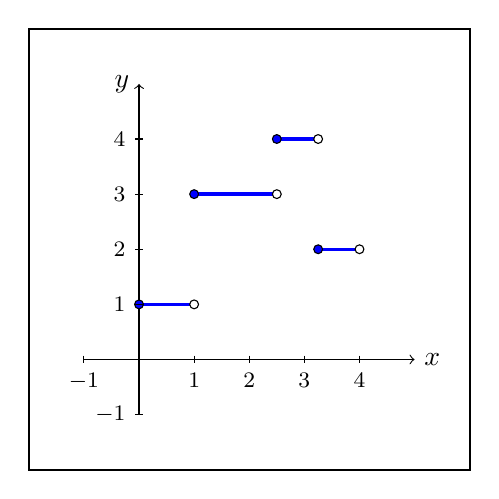
\begin{tikzpicture}[scale=0.7]
				
				\draw[thick] (-2,-2) rectangle (6, 6);
                % Eixos
                \draw[->] (-1,0) -- (5,0) node[right] {$x$};
                \draw[->] (0,-1) -- (0, 5) node[left] {$y$};
                                
                % Plot do gráfico
                \draw[domain=0:1,very thick,variable=\x,blue] plot ({\x},{1});
                \draw[domain=1:2.5,very thick,variable=\x,blue] plot ({\x},{3});
                \draw[domain=2.5:3.25,very thick,variable=\x,blue] plot ({\x},{4});
                \draw[domain=3.25:4,very thick,variable=\x,blue] plot ({\x},{2});
        		
        		% Bolinhas dos Intervalos
        		\draw[fill=blue] (0,1) circle (0.08);
        		\draw[fill=blue] (1,3) circle (0.08);
        		\draw[fill=blue] (2.5,4) circle (0.08);
        		\draw[fill=blue] (3.25,2) circle (0.08);
        		
        		\draw[fill=white] (1,1) circle (0.08);
        		\draw[fill=white] (2.5,3) circle (0.08);
        		\draw[fill=white] (3.25,4) circle (0.08);
        		\draw[fill=white] (4,2) circle (0.08);
        		                

                % Rótulos
                \foreach \i in {-1,1,2,3,4}{
                \draw (\i,2pt)--(\i, -2pt) node[below]{{\footnotesize $\i$}};
                }
                
                \foreach \i in {-1,1,2,3,4}{
                \draw (2pt,\i)--(-2pt, \i) node[left]{{\footnotesize $\i$}};
                }
                
                % Linhas trastejadas
                % \foreach \i in {1,2,3,4}{
                % \draw[dashed, help lines] (\i,0) -- (\i,\i);
                % }
                % \foreach \i in {1,2,3}{
                % \draw[dashed, help lines] (\i,\i) -- (\i,\i+1);
                % }  
            \end{tikzpicture}
	}{
	    \Fonte{Elaborado pelo autor}
	}	
    \end{figure} 
Agora pensemos na ideia de integral apresentada na disciplina de Cálculo Diferencial e Integral.
Se quiséssemos calcular a integral das funções acima somaríamos as áreas dos retângulos conforme ilustram as figuras a seguir.\\
 
    %Gráfico da função g
    \begin{figure}[!h]
	\centering
	\Caption{\label{fig:integral-função-simples-g-sobre-[0,4]} Área delimitada pelo gráfico da função $g =\dsum_{j = 1}^4 a_j\chi_{E_j}$}	
	\UECEfig{}{
	    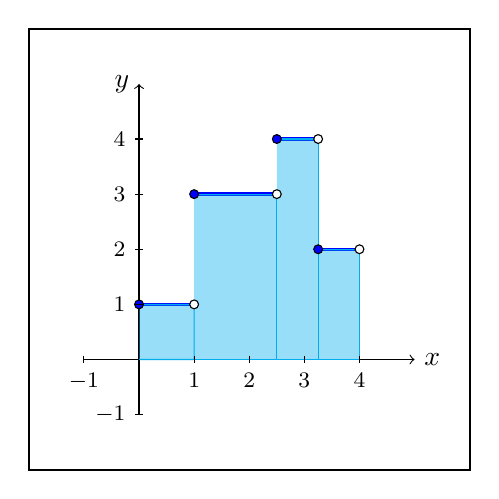
\begin{tikzpicture}[scale=0.7]
	    	\draw[thick] (-2,-2) rectangle (6, 6);
                % Eixos
                \draw[->] (-1,0) -- (5,0) node[right] {$x$};
                \draw[->] (0,-1) -- (0, 5) node[left] {$y$};
                                
                % Plot do gráfico	
				\draw[domain=0:1,very thick,variable=\x,blue] plot ({\x},{1});
				\draw[domain=1:2.5,very thick,variable=\x,blue] plot ({\x},{3});
				\draw[domain=2.5:3.25,very thick,variable=\x,blue] plot ({\x},{4});
				\draw[domain=3.25:4,very thick,variable=\x,blue] plot ({\x},{2});

				
				\filldraw [domain=0:1,smooth,variable=\x, cyan, fill opacity=0.4]  plot ({\x},{1})--(1,0)--(0,0);
	            \filldraw [domain=1:2.5,smooth,variable=\x, cyan, fill opacity=0.4]  plot ({\x},{3})--(2.5,0)--(1,0);
				\filldraw [domain=2.5:3.25,smooth,variable=\x, cyan, fill opacity=0.4]  plot ({\x},{4})--(3.25,0)--(2.5,0);
				\filldraw [domain=3.25:4,smooth,variable=\x, cyan, fill opacity=0.4]  plot ({\x},{2})--(4,0)--(3.25,0);
                
        		% Bolinhas dos Intervalos
				\draw[fill=blue] (0,1) circle (0.08);
				\draw[fill=blue] (1,3) circle (0.08);
				\draw[fill=blue] (2.5,4) circle (0.08);
				\draw[fill=blue] (3.25,2) circle (0.08);
				
				\draw[fill=white] (1,1) circle (0.08);
				\draw[fill=white] (2.5,3) circle (0.08);
				\draw[fill=white] (3.25,4) circle (0.08);
				\draw[fill=white] (4,2) circle (0.08);


                % Rótulos
                \foreach \i in {-1,1,2,3,4}{
                \draw (\i,2pt)--(\i, -2pt) node[below]{{\footnotesize $\i$}};
                }
                
                \foreach \i in {-1,1,2,3,4}{
                \draw (2pt,\i)--(-2pt, \i) node[left]{{\footnotesize $\i$}};
                }
                
                % Linhas trastejadas
                % \foreach \i in {1,2,3,4}{
                % \draw[dashed, help lines] (\i,0) -- (\i,\i);
                % }
                % \foreach \i in {1,2,3}{
                % \draw[dashed, help lines] (\i,\i) -- (\i,\i+1);
                % }  
            \end{tikzpicture}
	}{
	    \Fonte{Elaborado pelo autor}
	}	
    \end{figure} 
Note que em ambos os casos estamos, basicamente, aplicando o valor $a_j$ na medida do conjunto $E_j$ correspondente onde $j$ é o número de partições do domínio. Com isso, temos a definição a seguir:
\begin{env}{Definição}
\label{def:integral-função-naonegativa-simples}
    Se $\varphi$ é uma função simples de $M^+(X, \cc)$ com a representação 
    $\displaystyle\varphi =  \sum_{j = 1}^n a_j\chi_{E_j},$ então a integral da função $\varphi$ com respeito à medida $\mu$ é o valor real estendido
    \linebreak $
    \displaystyle\int\varphi d\mu = \sum_{j = 1}^n a_j\mu(E_j)
    $
    \cite[p.28, tradução nossa]{bartle}
    \footnote{No original: 
    	If $\phi$ is a simple function in $M^+(X, \textbf{X})$ [...], we define the integral of $\phi$ with respect to
    	$\mu$ to be the extended real number  
    	$
    	\displaystyle\int\varphi d\mu = \sum_{j = 1}^n a_j\mu(E_j)
    	$.
    }.
\end{env}

Para a \ref{def:integral-função-naonegativa-simples} empregamos a convenção que $0 \cdot (+\infty) = 0$.
Isso é feito para garantir que a função identicamente nula tenha integral nula independentemente da medida ser finita ou não.
A seguir, veremos propriedades elementares sobre a integral de funções simples.

\begin{comment}
	

Antes disso, considere um espaço de medida $(X, \cc, \mu)$.
Seja  $\{E_n\}$ uma partição de $X$ com $n \in I_5$ conforme a representação a seguir.\pagebreak
\begin{figure}[h]
	\centering
	\Caption{\label{fig:particao-E-de-X} Partição $\{E_n\}$ do conjunto $X$} 
	\UECEfig{}{
		% Partição de X por E_n
		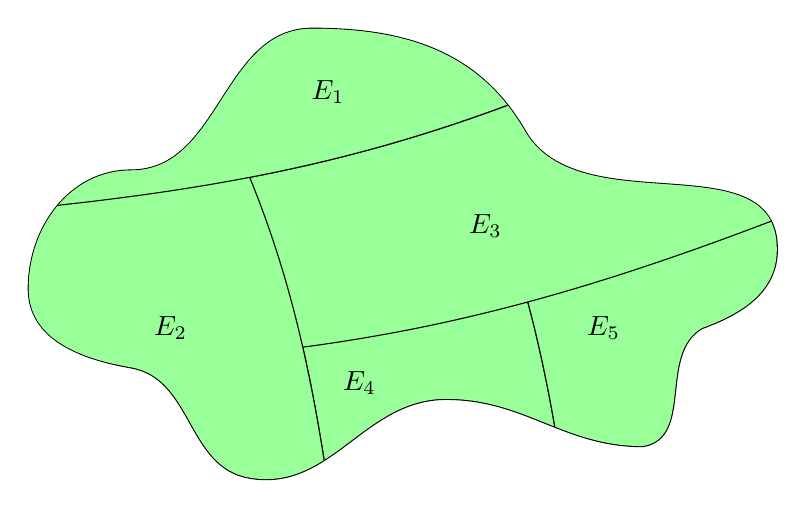
\begin{tikzpicture}
			% Define coordenadas que serão utilizadas posteriormente
			\path
			coordinate (aux0) at (0,1.5)
			coordinate (aux1) at (0,3.5)
			coordinate (aux2) at (10,3.5)
			coordinate (aux3) at (9,6)
			coordinate (aux4) at (4,0)
			coordinate (aux5) at (7,0)
			coordinate (aux6) at (2,6)
			coordinate (aux7) at (5,6)
			coordinate (esp1) at (0.2,2.5)
			coordinate (esp2) at (1.5,1.5)
			coordinate (esp3) at (3,0.1)
			coordinate (esp4) at (5.5,1.1)
			coordinate (esp5) at (8,0.5)
			coordinate (esp6) at (8.75,2)
			coordinate (esp7) at (9.7,3)
			coordinate (esp8) at (6.5,4.5)
			coordinate (esp9) at (3.8,5.8)
			coordinate (esp10) at (1.5,4)
			coordinate (nome) at (0, 6)
			;
			% Desenha curvas com angulação de saida e entrada
			\draw[line width=0.8pt]
			(esp1) to[out=-90,in=170]
			(esp2) to[out=-10,in=170]
			(esp3) to[out=-10,in=180]
			(esp4) to[out=0,in=180]
			(esp5) to[out=10,in=-150]
			(esp6) to[out=20,in=-90]
			(esp7) to[out=90,in=-60]
			(esp8) to[out=120,in=0]
			(esp9) to[out=180,in=0]
			(esp10) to[out=180,in=90]
			cycle;    
			% Limita a figura às coordenadas citadas
			\clip
			(esp1) to[out=-90,in=170]
			(esp2) to[out=-10,in=170]
			(esp3) to[out=-10,in=180]
			(esp4) to[out=0,in=180]
			(esp5) to[out=10,in=-150]
			(esp6) to[out=20,in=-90]
			(esp7) to[out=90,in=-60]
			(esp8) to[out=120,in=0]
			(esp9) to[out=180,in=0]
			(esp10) to[out=180,in=90]
			cycle;    
			
			\draw[fill=green!40]
			(aux4) to[bend right=10]
			(aux6) --
			(aux7) to[bend left=10]
			(aux5) -- cycle;
			\draw[fill=green!40]
			(aux5) to[bend right=10]
			(aux7) --
			(10,6) --
			(10,0) -- cycle;
			\draw[fill=green!40]
			(aux0) -- 
			(aux1) to[bend right=10]
			(aux3) --
			(10,6) -- 
			(aux2) to[bend left=10] cycle;
			\draw[fill=green!40]
			(0,0) -- 
			(aux4) to[bend right=10]
			(aux6) --
			(0,6) -- 
			(0,0) -- cycle;
			\draw[fill=green!40]
			(0,6) -- 
			(aux1) to[bend right=10]
			(aux3) --
			(0,6) -- cycle;
			\node at (4,5) {$E_1$};  
			\node at (2,2) {$E_2$};  
			\node at (6,3.3) {$E_3$};  
			\node at (4.4,1.3) {$E_4$};  
			\node at (7.5,2) {$E_5$};
			\node at (0.1,5.5) {$X$};  
			
		\end{tikzpicture}
		
	}{
		\Fonte{Elaborado pelo autor}
	}   
\end{figure}

\hspace{-2cm}Tome também uma outra partição $\{F_m\}$ onde $m \in I_6$.\\

\begin{figure}[h!]
	\centering
	\Caption{\label{fig:particao-F-de-X} Partição $\{F_m\}$ do conjunto $X$} 
	\UECEfig{}{
		% Partição F_m
		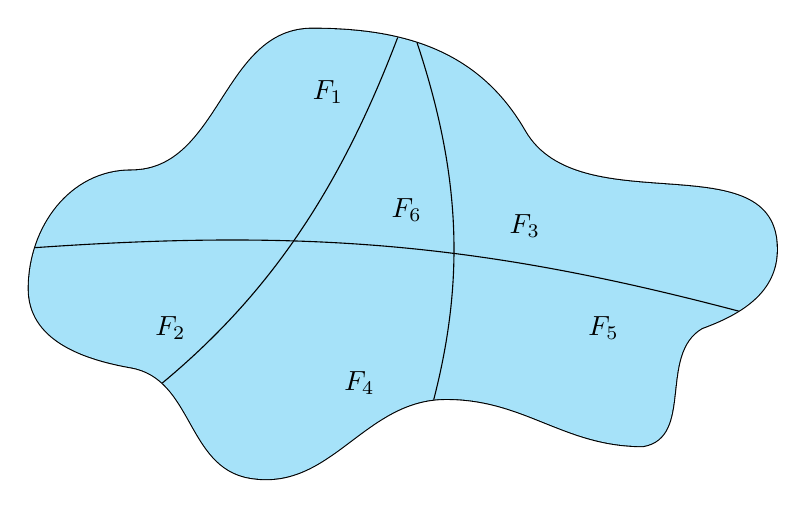
\begin{tikzpicture}
			% Define coordenadas que serão utilizadas posteriormente
			\path
			coordinate (aux0) at (1.1,2)
			coordinate (aux1) at (0,3.5)
			coordinate (aux2) at (10,3.5)
			coordinate (aux3) at (9,6)
			coordinate (aux4) at (4,0)
			coordinate (aux5) at (7,0)
			coordinate (aux6) at (2,6)
			coordinate (aux7) at (5,6)
			coordinate (aux8) at (11,2)
			coordinate (aux9) at (3,8.2)
			coordinate (esp1) at (0.2,2.5)
			coordinate (esp2) at (1.5,1.5)
			coordinate (esp3) at (3,0.1)
			coordinate (esp4) at (5.5,1.1)
			coordinate (esp5) at (8,0.5)
			coordinate (esp6) at (8.75,2)
			coordinate (esp7) at (9.7,3)
			coordinate (esp8) at (6.5,4.5)
			coordinate (esp9) at (3.8,5.8)
			coordinate (esp10) at (1.5,4)
			coordinate (nome) at (0, 6)
			;
			% Desenha curvas com angulação de saida e entrada
			\draw[line width=0.8pt]
			(esp1) to[out=-90,in=170]
			(esp2) to[out=-10,in=170]
			(esp3) to[out=-10,in=180]
			(esp4) to[out=0,in=180]
			(esp5) to[out=10,in=-150]
			(esp6) to[out=20,in=-90]
			(esp7) to[out=90,in=-60]
			(esp8) to[out=120,in=0]
			(esp9) to[out=180,in=0]
			(esp10) to[out=180,in=90]
			cycle;    
			% Limita a figura às coordenadas citadas
			\clip
			(esp1) to[out=-90,in=170]
			(esp2) to[out=-10,in=170]
			(esp3) to[out=-10,in=180]
			(esp4) to[out=0,in=180]
			(esp5) to[out=10,in=-150]
			(esp6) to[out=20,in=-90]
			(esp7) to[out=90,in=-60]
			(esp8) to[out=120,in=0]
			(esp9) to[out=180,in=0]
			(esp10) to[out=180,in=90]
			cycle;    
			
			\draw[fill=cyan!35] 
			(0,0) rectangle (10,6);
			\draw
			(0,0) 
			to[bend right = 20] 
			(aux7)
			to[bend right = 22] 
			(aux1);
			\draw
			(0,3) 
			to[bend left = 10] 
			(10,2)
			to[bend right = 10]
			(5,-6);
			\draw
			(5,0) 
			to[bend right = 20] 
			(aux7)
			to[bend right = 22] 
			(aux1);
			
			
			% Rótulos
			\node at (4,5) {$F_1$};  
			\node at (2,2) {$F_2$};  
			\node at (6.5,3.3) {$F_3$};  
			\node at (4.4,1.3) {$F_4$};  
			\node at (7.5,2) {$F_5$};  
			\node at (5,3.5) {$F_6$};
		\end{tikzpicture}
		
	}{
		\Fonte{Elaborado pelo autor}
	}   
\end{figure}
Claramente, ao observar as figuras acima, podemos ver que $E_3$ possui interseção com $F_j$ para todo $j \in I_6$.
Assim, $E_5 = \displaystyle \bigcup_{j = 1}^6 (F_j\cap E_5)$ com $(F_j\cap E_5) = \varnothing,\ \forall j \in I_6$. 
Logo, 
$$
\mu(E_5) = \mu\left(\bigcup_{j = 1}^6 (F_j\cap E_5)\right)
= 
\sum_{j=1}^{6}\mu(F_j\cap E_5)
$$
A igualdade acima é valida mesmo se o conjunto em questão não tiver interseção com todos os outros da partição.
Neste caso, a interseção com os demais será vazia e soma associada à eles é 0.
Basta observar, por exemplo, o conjunto $E_1$ que tem interseção com $F_1, F_6$ e $F_3$, mas não se intersecta com $F_2, F_4$ e $F_5$.
Deste modo,
$$
\sum_{j=1}^{6}\mu(F_j\cap E_3)
= \mu(F_1\cap E_3) + \mu(F_6\cap E_3) + \mu(F_3\cap E_3)
= \mu(E_3)
$$
Pois, $\mu(F_2\cap E_3) = \mu(F_4\cap E_3) = \mu(F_5\cap E_3) = 0$.
\end{comment}

\begin{env}{Teorema}
	\label{teo:aritmetica-com-integrais-de-funções-simples}
    Se $\varphi$ e $\psi$ são funções simples do espaço $M^+(X,\cc)$ e $c\geq0$ é uma constante real, então
    $
    \displaystyle \int c\varphi d\mu = c \int \varphi d\mu
    $
	e
    $
    \displaystyle \int (\varphi + \psi) d\mu = \int \varphi d\mu + \int \psi d\mu
    $ \cite{bartle}.
\end{env}
\begin{prova}
    Representaremos as funções simples não negativas por $\varphi = \dsum_{j = 1}^n a_j\chi_{E_j}$ e $\psi = \dsum_{k = 1}^m b_k\chi_{F_k}$.
    Primeiro, mostraremos que vale a multiplicação por escalar.
    Assim, caso $c = 0$, o resultado é verdadeiro trivialmente. 
    Supondo $c> 0$, temos que
    $$\int c \varphi\ d\mu = \dsum_{j = 1}^n c a_j\mu(E_j) = c \dsum_{j = 1}^n a_j\mu(E_j) = c\int \varphi \ d\mu.$$
    Com isso, concluímos que $\displaystyle \int c \varphi\ d\mu = c\int \varphi \ d\mu.$ 
 	
    Agora provaremos que a integral da soma é igual a soma das integrais. 
    Assim, dadas as representações padrão de $\varphi$ e $\psi$, vemos que
    \begin{equation}
    	\label{eq:somatorio funções simples}
    	\varphi +\psi
    	=
    	\dsum_{j = 1}^n a_j\chi_{E_j}
    	+
    	\dsum_{k = 1}^m b_k\chi_{F_k}
    \end{equation}
    Como $\{E_n\}$ e $\{F_k\}$ são ambas partições de $X$, pela \ref{prop: igualdade da caracteristica como medida} temos que
    $\chi_{E_j} = \dsum_{k = 1}^m \chi_{(E_j \cap F_k)}$ e 
    $\chi_{F_k} = \dsum_{j = 1}^n \chi_{(E_j \cap F_k)}$.
    Substituindo na equação \ref{eq:somatorio funções simples}, obtemos    
    \begin{align*}
    	\dsum_{j = 1}^n a_j\chi_{E_j}
    	+
    	\dsum_{k = 1}^m b_k\chi_{F_k}
    	= &
    	\dsum_{j = 1}^n a_j\left(\dsum_{k = 1}^m \chi_{(E_j \cap F_k)}\right)
    	+
    	\dsum_{k = 1}^m b_k\left(\dsum_{j = 1}^n \chi_{(E_j \cap F_k)}\right)\\
    	= &
    	\dsum_{j = 1}^n\dsum_{k = 1}^m a_j\chi_{(E_j \cap F_k)}
    	+
    	\dsum_{k = 1}^m \dsum_{j = 1}^n b_k\chi_{(E_j \cap F_k)}\\
	\end{align*}
	\begin{align*}
		= &
		\dsum_{j = 1}^n\dsum_{k = 1}^m 
		\left(a_j\chi_{(E_j \cap F_k)}
		+
		b_k\chi_{(E_j \cap F_k)}\right)\\
		= &
		\dsum_{j = 1}^n\dsum_{k = 1}^m 
		(a_j + b_k)\chi_{(E_j \cap F_k)}.
	\end{align*}
    Com isso, concluímos que
    $$
    \varphi + \psi = \dsum_{j = 1}^n\dsum_{k = 1}^m(a_j + b_k)\chi_{E_j \cap F_k}.
    $$
    Entretanto, essa representação não é, necessariamente, a representação padrão apresentada na \ref{def:integral-função-naonegativa-simples}, pois 
    nada garante, previamente, que $a_j + b_k$ sejam distintos para $j \in I_n$ e $k \in I_m$.
    Com isso, sejam $c_h$, com $h \in I_p$, números distintos do conjunto $\{a_j + b_k; \ (j,k) \in I_n \times I_m\}$ e $G_h$ a união de todos os conjuntos $E_j \cap F_k \neq \varnothing$ tal que $a_j + b_k = c_h$.
    Assim, 
    $$
    G_h = \bigcup_{\begin{minipage}{1.4cm}
        \fontsize{8}{5}\selectfont
        \centering
        $j,k$
        $a_j + b_k = c_h$
    \end{minipage}} E_j \cap F_k
    $$
    A notação utilizada acima indica que a soma é realizada sobre todos os índices $j$ e $k$ tais que $a_j + b_k =c_h$.
    Como $(E_j \cap F_k) \cap (E_l \cap F_p)= \varnothing$ para todo $j \neq l$ e $k \neq p$ , temos que 
    $$
    \mu(G_h) = \mu\left(\bigcup_{
        j,k\atop
        a_j + b_k = c_h} E_j \cap F_k
    \right)
    = 
    \sum_{
        j,k\atop
        a_j + b_k = c_h} \mu(E_j \cap F_k)
    $$
    Desta forma, conseguimos encontrar uma representação padrão que é dada por 
    $\displaystyle \varphi + \psi = \sum_{h =1}^p c_h\chi_{G_h}$.
    Logo, temos que 
    \begin{align*}
        \int(\varphi + \psi) d\mu = \sum_{h =1}^p c_h\mu(G_h)
        = & 
        \sum_{h = 1}^p\sum_{ j,k\atop a_j + b_k = c_h}c_h \mu(E_j \cap F_k)\\
        = &
        \sum_{h = 1}^p\sum_{ j,k\atop a_j + b_k = c_h}(a_j + b_k) \mu(E_j \cap F_k)\\
        = &
        \sum_{j = 1}^n\sum_{k = 1}^m(a_j + b_k) \mu(E_j \cap F_k)\\
        = &
        \sum_{j = 1}^n\sum_{k = 1}^m a_j \mu(E_j \cap F_k) + \sum_{j = 1}^n\sum_{k = 1}^m b_k \mu(E_j \cap F_k)
    \end{align*}
	Pela \ref{prop: medida com partição}, temos
	$
	\displaystyle
	\mu(E_j) = \sum_{k = 1}^m \mu(E_j \cap F_k)
	$
    e
    $\displaystyle \mu(F_k) = \sum_{j = 1}^n \mu(E_j \cap F_k)$.
    Empregando estes resultados ao que foi desenvolvido anteriormente obtemos
    $$
    \sum_{j = 1}^n\sum_{k = 1}^m a_j \mu(E_j \cap F_k) + \sum_{j = 1}^n\sum_{k = 1}^m b_k \mu(E_j \cap F_k)
    =
    \sum_{j = 1}^n a_j \mu(E_j) + \sum_{k = 1}^m b_k \mu(F_k)
    =
    \int \varphi d\mu + \int \psi d\mu
    $$
    Segue que $\displaystyle\int(\varphi + \psi) d\mu = \int \varphi d\mu + \int \psi d\mu$ como queríamos.
\end{prova}


% Lemas para o teorema

\begin{env}{Lema}
	\label{lem:medida-da-intersecao-de-um-fixado}
	Se $\mu$ é uma medida sobre $X$ e fixemos um elemento $A$ de $\cc$, então a função $\lambda$ definida por $\lambda(E) = \mu(A\cap E), \ \forall\  E \in \cc$ também é uma medida sobre $X$ \cite{bartle}.
\end{env}
\begin{prova}
	Basta mostrar que $\lambda$ satisfaz as condições impostas na  \ref{def:medida}.
	Com isso, se $E = \varnothing$, então
	$$
	\lambda(\varnothing) = \mu(A \cap \varnothing) = \mu(\varnothing) = 0
	$$
	Como $A$ e $E$ são elementos de $\cc$, então $A \cap E$ também está em $\cc$.
	Assim, por $\mu$ ser uma medida, temos que $\mu(A\cap E) \geq 0$ acarretando que $\lambda(E) \geq 0$.
	Por fim, tomemos uma sequência de elementos disjuntos $(E_n)$ em $\cc$.
	Se $A \cap E_j \neq \varnothing$ para algum $j \in \N$ 
	não há o que fazer, pois $(A \cap E_j) \subset E_j \in \cc$.
	Caso $A \cap E_j = \varnothing$ para todo $j \in \N$, então $\displaystyle \left( \bigcup_{n \in \N} E_n\right) \cap A = \varnothing$.
	Com isso, 
	
	\begin{align*}
		\left( \bigcup_{n \in \N} E_n\right) \cap A
		= &
		(E_1 \cup E_2 \cup \cdots \cup E_n \cup \cdots) \cap A\\
		= &
		(E_1 \cap A )\cup (E_2 \cap A) \cup \cdots \cup (E_n\cap A) \cup \cdots \\
		= &
		\bigcup_{n \in \N} (E_n\cap A)    
	\end{align*}
	%   
	Segue então que
	$$
	\lambda\left( \bigcup_{n \in \N} E_n\right)
	=
	\mu\left(\left( \bigcup_{n \in \N} E_n\right) \cap A\right)
	=
	\mu\left( \bigcup_{n \in \N} (E_n\cap A) \right)
	=
	\sum_{j = 1}^\infty \mu(E_j \cap A)
	= 
	\sum_{j = 1}^\infty \lambda(E_j)
	$$
	Desta forma, concluímos que a função $\lambda$ acima definida é uma medida.
\end{prova}

\begin{env}{Lema}
	\label{lem:medida-gerada-por-medidas-e-numeros-reais}
	Se $\mu_1, ..., \mu_n$ são medidas sobre $X$ e $a_1, ... , a_n$ são números reais não negativos, então a função $\lambda$ definida por
	$\lambda(E) = \dsum_{j =1}^n a_j\mu_j(E), \forall\  E \in \cc$ também é uma medida sobre $X$  \cite{bartle}.
\end{env}
\begin{prova}
	Como $\mu_j$ é uma medida para todo $j \in I_n$ e cada $a_j$ é maior ou igual à zero, temos que cada $a_j\mu_j(E) \geq 0$.
	Desta maneira, $\lambda(E) = \displaystyle \sum_{j = 1}^n a_j\mu_j(E) \geq 0$.
	Além disso, podemos observar que $\lambda(\varnothing) = \displaystyle \sum_{j =1}^n a_j\mu_j(\varnothing) = 0$.
	Tomemos uma sequência disjunta $(E_p)$ de elementos de $\cc$.
	Logo, 
	$$
	\lambda\left(\bigcup_{p \in \N} E_p\right)
	=
	\sum_{j = 1}^n a_j\mu_j\left(\bigcup_{p \in \N} E_p\right)
	=
	\sum_{j = 1}^n a_j\left(\sum_{p = 1}^\infty\mu_j(E_p)\right)
	=
	\sum_{p = 1}^\infty\left(\sum_{j = 1}^na_j\mu_j(E_p)\right)
	=
	\sum_{p = 1}^{\infty}\lambda(E_p)
	$$
	\begin{comment}
	Afirmamos que $\displaystyle \sum_{j = 1}^n a_j\left(\sum_{p = 1}^\infty\mu_j(E_p)\right) = \sum_{p = 1}^\infty\left(\sum_{j = 1}^na_j\mu_j(E_p)\right)$.
	Com efeito, 
	\begin{align*}
	\sum_{j = 1}^n a_j\left(\sum_{p = 1}^\infty\mu_j(E_p)\right)
	= &
	\sum_{j = 1}^n a_j\left(\lim_{m \to +\infty}\sum_{p = 1}^m\mu_j(E_p)\right)\\
	= &
	\lim_{m \to +\infty}\left[\sum_{j = 1}^n a_j\left(\sum_{p = 1}^m\mu_j(E_p)\right)\right]\\
	= &
	\lim_{m \to +\infty}\left[a_1\left(\sum_{p = 1}^m\mu_1(E_p)\right)+ \cdots + a_n\left(\sum_{p = 1}^m\mu_n(E_p)\right)\right]\\
	= &
	\lim_{m \to +\infty}\left(\sum_{p = 1}^ma_1\mu_1(E_p)+ \cdots + \sum_{p = 1}^ma_n\mu_n(E_p)\right)\\
	= &
	\lim_{m \to +\infty}\sum_{p = 1}^m \left(a_1\mu_1(E_p)+ \cdots + a_n\mu_n(E_p)\right)\\
	= &
	\lim_{m \to +\infty}\sum_{p = 1}^m \left(\sum_{j = 1}^na_j\mu_j(E_p)\right)\\
	= &
	\sum_{p = 1}^\infty \left(\sum_{j = 1}^na_j\mu_j(E_p)\right)\\
\end{align*}		
	\end{comment}
	
\begin{comment}
		Disso tudo, obtemos que 
	$$
	\lambda\left(\bigcup_{p \in \N} E_p\right)
	=
	\sum_{j = 1}^n a_j\left(\sum_{p = 1}^\infty\mu_j(E_p)\right)
	=
	\sum_{p = 1}^\infty \left(\sum_{j = 1}^na_j\mu_j(E_p)\right)
	=
	\sum_{p = 1}^\infty \lambda(E_p)
	$$
\end{comment}

	Como $\lambda$ satisfaz todas as condições impostas na  \ref{def:medida} concluímos que $\lambda$ é uma medida.    
\end{prova}

\begin{env}{Teorema}
	\label{teo:medida-atraves-de-uma-integral}
	Se $\phi$ é uma função simples com  a representação padrão dada por $\phi = \dsum_{j = 1}^n a_j\chi_{E_j}$, então a função $\lambda: \cc \to \xreta$ definida por
	$
	\displaystyle\lambda(E) = \int \varphi\chi_E\ d\mu
	$
	para todo $E \in \cc$ é uma medida sobre $\cc$
	\cite{bartle}. 
\end{env}

\begin{prova}
	De maneira análoga ao  \ref{teo:aritmetica-com-integrais-de-funções-simples}
	podemos verificar que 
	$
	\varphi\chi_E = \dsum_{j = 1}^n a_j\chi_{E_j \cap E}.
	$
	Assim, temos que 
	\begin{align*}
		\lambda(E) 
		= \int \varphi\chi_E d\mu
		= \int\left(\sum_{j = 1}^n a_j\chi_{E_j \cap E}\right)d\mu
		= \sum_{j = 1}^n\left(a_j\int \chi_{E_j \cap E}d\mu\right) 
		= \sum_{j = 1}^n a_j\mu(E_j\cap E)
	\end{align*}
	Pelo  \ref{lem:medida-da-intersecao-de-um-fixado} a aplicação que leva 
	$E \to \mu(E_j\cap E)$ é uma medida para cada $j \in I_n$.
	Disso, concluímos que $\lambda$ pode ser expressada por uma combinação linear de medidas sobre $\cc$.
	Segue, pelo  \ref{lem:medida-gerada-por-medidas-e-numeros-reais}, que 
	$\lambda$ também é uma medida sobre $\cc$.
\end{prova}

% Mostrar que existe uma função simples que aproxima uma função
\section{A Integral de Funções Não-Negativas}

Até aqui trabalhos apenas com integrais de funções simples.
Nesta seção, desejamos expandir o conceito de integral para uma função qualquer não negativa.
Vale ressaltar que a perspectiva que traremos aqui é a de Lebesgue.
Com o intuito de enfatizar a diferença da construção, vamos lembrar da construção feita por Riemann.
Considere a função $f: \R \to \R$ tal que $f(x) = \mathrm{sen}(x) + 3$.
Claramente não é uma função simples, pois não possui uma quantidade finita de valores. 
Nosso objetivo, agora, é tentar calcular a integral dessa função com o que construímos até aqui.
Para facilitar, observe o gráfico dessa função no intervalo $[0,4]$ apresentado na figura \ref{fig:gráfico da função sen x + 3}.

\begin{figure}[h!]
	\centering
	\Caption{\label{fig:gráfico da função sen x + 3} Gráfico da função $f(x) = \textrm{sen}(x) + 3$} 
	\UECEfig{}{
		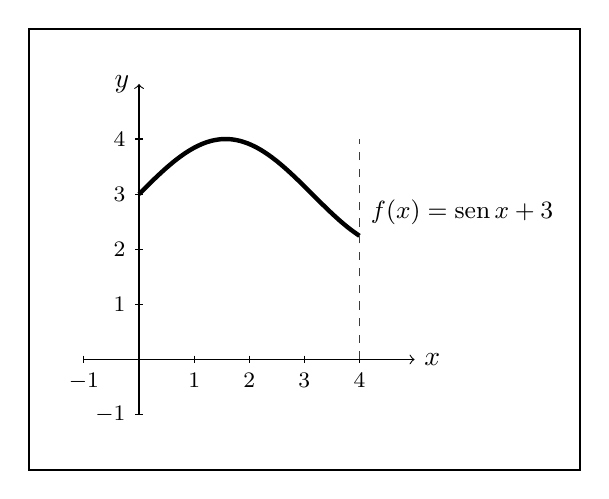
\begin{tikzpicture}[scale=0.7]
			\draw[thick] (-2,-2) rectangle (8, 6);
			% Eixos
			\draw[->] (-1,0) -- (5,0) node[right] {$x$};
			\draw[->] (0,-1) -- (0, 5) node[left] {$y$};
			
			% Plot do gráfico
			%	\draw[domain=0:1,very thick,variable=\x,blue] plot ({\x},{1});
			%	\draw[domain=1:2,very thick,variable=\x,blue] plot ({\x},{2});
			%	\draw[domain=2:3,very thick,variable=\x,blue] plot ({\x},{3});
			%	\draw[domain=3:4,very thick,variable=\x,blue] plot ({\x},{4});
			%	
			
			%	% Retangulos
			%	\foreach \i in {0, 1,2,3}{
				%		\draw[fill=blue!30, dashed](\i,0) rectangle (\i+1,\i +1);
				%	}
			%	
			% Bolinhas de intervalos aberto e fechado
			%	\foreach \i in {1,2,3}{
				%		\draw[fill=white] (\i,\i+1) circle (0.08);
				%	}
			%	\foreach \i in {1,2,3,4}{
				%		\draw[fill=blue] (\i,\i) circle (0.08);
				%	}
			%	
			% Rótulos
			\foreach \i in {-1,1,2,3,4}{
				\draw (\i,2pt)--(\i, -2pt) node[below]{{\footnotesize $\i$}};
			}
			
			\foreach \i in {-1,1,2,3,4}{
				\draw (2pt,\i)--(-2pt, \i) node[left]{{\footnotesize $\i$}};
			}
			
			
%			\fill[domain=0:4,smooth,variable=\x, cyan, fill opacity=0.4]  plot ({\x},{3+sin(\x r)})--(4,0)--(0,0);
%			% Yes, this is drawn twice, but I wanted the shading to match the over/under pictures following.
			
			
			\draw[domain=0:4,smooth,variable=\x, ultra thick]  plot ({\x},{3+sin(\x r)})  node[above right] {{\small $f(x) = \textrm{sen}\,x + 3$}};
			\draw[dashed, green!40!black]  (4,0)--(4,4);
			
			
			
		\end{tikzpicture}
		
	}{
		\Fonte{Elaborado pelo autor}
	}   
\end{figure}
\hspace{-2cm}Tomemos a função simples 
$$
\phi_2(x) =\sum_{j = 1}^{2} a_j\chi_{E_j}
$$
onde $a_1 = f(0), a_2 = f(2); E_1 = [0, 2)$ e $E_2 = [2, 4]$.
Assim, ao calcularmos sua integral, vemos não há preenchimento total da área delimitada pelo gráfico da função $f$, mas se aproxima com um erro conforme a figura \ref{fig: integral da funçao phi 2}.

\begin{figure}[h!]
	\centering
	\Caption{\label{fig: integral da funçao phi 2} Integral da função $\phi_2$} 
	\UECEfig{}{
		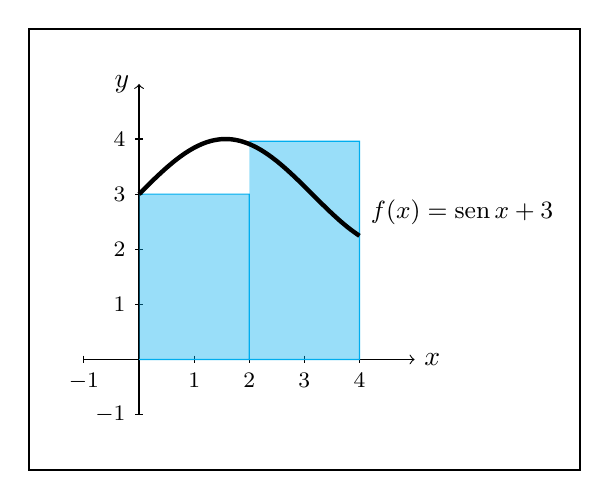
\begin{tikzpicture}[scale=0.7]
			\draw[thick] (-2,-2) rectangle (8, 6);
			% Eixos
			\draw[->] (-1,0) -- (5,0) node[right] {$x$};
			\draw[->] (0,-1) -- (0, 5) node[left] {$y$};
			
			% Rótulos
			\foreach \i in {-1,1,2,3,4}{
				\draw (\i,2pt)--(\i, -2pt) node[below]{{\footnotesize $\i$}};
			}
			
			\foreach \i in {-1,1,2,3,4}{
				\draw (2pt,\i)--(-2pt, \i) node[left]{{\footnotesize $\i$}};
			}
				% Plot do gráfico
			\filldraw[domain=0:2,smooth,variable=\x, cyan, fill opacity=0.4] plot ({\x},{3})--(2,0)--(0,0);
			\filldraw[domain=2:4,smooth,variable=\x, cyan, fill opacity=0.4] plot ({\x},{3.96})--(4,0)--(2,0);	
			
			\draw[domain=0:4,smooth,variable=\x, ultra thick]  plot ({\x},{3+sin(\x r)})  node[above right] {{\small $f(x) = \textrm{sen}\,x + 3$}};
	
		\end{tikzpicture}
		
	}{
		\Fonte{Elaborado pelo autor}
	}   
\end{figure}

\hspace{-2cm} Vamos escolher outra função simples $\phi_4$ tal que $\phi_4 =\sum_{j = 1}^{4} a_j\chi_{E_j}$
onde 
$E_1 = [0, 1),\ 
 E_2 = [1, 2),\ 
 E_3 = [2, 3),\ 
 E_1 = [3, 4],\ 
 a_1 = f(0), \ 
 a_2 = f(1), \ 
 a_3 = f(3)$ e $a_4 = f(4)$.
Desta forma, com o dobro de valores da função $\phi_2$ escolhida anteriormente podemos observar que a integral de $\phi_4$, exibida na figura \ref{fig:integral da função phi 4}, mais se aproxima da integral da função $f$.
\begin{figure}[h!]
	\centering
	\Caption{\label{fig:integral da função phi 4} Integral da função $\phi_4$} 
	\UECEfig{}{
		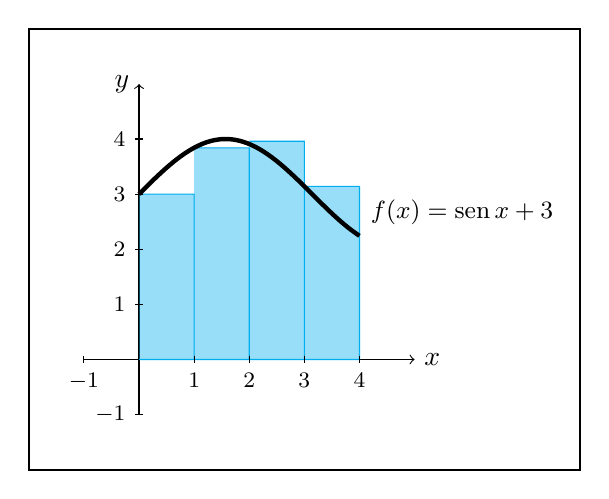
\begin{tikzpicture}[scale=0.7]
			\draw[thick] (-2,-2) rectangle (8, 6);
			% Eixos
			\draw[->] (-1,0) -- (5,0) node[right] {$x$};
			\draw[->] (0,-1) -- (0, 5) node[left] {$y$};
			
			% Plot do gráfico
			\filldraw [domain=0:1,smooth,variable=\x, cyan, fill opacity=0.4]  plot ({\x},{3})--(1,0)--(0,0);
			\filldraw[domain=1:2,smooth,variable=\x, cyan, fill opacity=0.4] plot ({\x},{3.84})--(2,0)--(1,0);	
			\filldraw[domain=2:3,smooth,variable=\x, cyan, fill opacity=0.4] plot ({\x},{3.96})--(3,0)--(2,0);
			\filldraw[domain=3:4,smooth,variable=\x, cyan, fill opacity=0.4] plot ({\x},{3.14})--(4,0)--(3,0);
					
			% Rótulos
			\foreach \i in {-1,1,2,3,4}{
				\draw (\i,2pt)--(\i, -2pt) node[below]{{\footnotesize $\i$}};
			}
			
			\foreach \i in {-1,1,2,3,4}{
				\draw (2pt,\i)--(-2pt, \i) node[left]{{\footnotesize $\i$}};
			}
			
			\draw[domain=0:4,smooth,variable=\x, ultra thick]  plot ({\x},{3+sin(\x r)})  node[above right] {{\small $f(x) = \textrm{sen}\,x + 3$}};
			
		\end{tikzpicture}
		
	}{
		\Fonte{Elaborado pelo autor}
	}   
\end{figure}
Para finalizarmos esta ideia, dobremos a quantidade de valores e escolhamos outra função 
$\phi_8 =\displaystyle\sum_{j = 1}^{8} a_j\chi_{E_j}$ 
onde 
$E_1 = [0, 0.5),\
 E_2 = [0.5, 1),\ 
 E_3 = [1, 1.5),\ 
 E_4 = [1.5, 2),\ 
 E_5 = [2,2.5), \ 
 E_6 = [2.5, 3), \ 
 E_7 = [3, 2.5), \ 
 E_8 = [3.5, 4]$ 
e
$a_1 = f(0),\ 
 a_2 = f(0.5),\ 
 a_3 = f(1), \ 
 a_4 = f(1.5),\ 
 a_5 = f(2.5), \ 
 a_6 = f(3), \ 
 a_7 = f(3.5)$ e $a_8 = f(4)$.
A integral da função $\phi_8$ está representada na figura 
figura \ref{fig:integrla da função phi 8}.
\begin{figure}[h!]
	\centering
	\Caption{\label{fig:integrla da função phi 8} Integral da função $\phi_8$} 
	\UECEfig{}{
		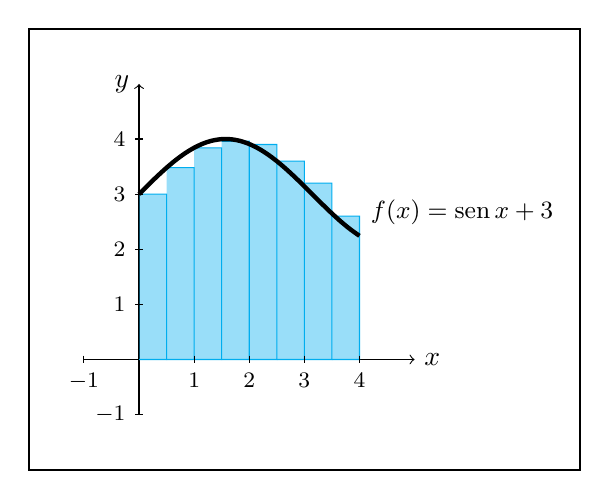
\begin{tikzpicture}[scale=0.7]
			\draw[thick] (-2,-2) rectangle (8, 6);
			% Eixos
			\draw[->] (-1,0) -- (5,0) node[right] {$x$};
			\draw[->] (0,-1) -- (0, 5) node[left] {$y$};
			
			% Plot do gráfico
			\filldraw [domain=0:0.5,smooth,variable=\x, cyan, fill opacity=0.4]  plot ({\x},{3})--(0.5,0)--(0,0);
			
			\filldraw [domain=0.5:1,smooth,variable=\x, cyan, fill opacity=0.4]  plot ({\x},{3.48})--(1,0)--(0.5,0);
			
			\filldraw[domain=1:1.5,smooth,variable=\x, cyan, fill opacity=0.4] plot ({\x},{3.84})--(1.5,0)--(1,0);	
			
			\filldraw[domain=1.5:2,smooth,variable=\x, cyan, fill opacity=0.4] plot ({\x},{3.96})--(2,0)--(1.5,0);
			
			\filldraw[domain=2:2.5,smooth,variable=\x, cyan, fill opacity=0.4] plot ({\x},{3.9})--(2.5,0)--(2,0);
			
			\filldraw[domain=2.5:3,smooth,variable=\x, cyan, fill opacity=0.4] plot ({\x},{3.6})--(3,0)--(2.5,0);
			
			\filldraw[domain=3:3.5,smooth,variable=\x, cyan, fill opacity=0.4] plot ({\x},{3.2})--(3.5,0)--(3,0);
			
			\filldraw[domain=3.5:4,smooth,variable=\x, cyan, fill opacity=0.4] plot ({\x},{2.6})--(4,0)--(3.5,0);
			
			% Rótulos
			\foreach \i in {-1,1,2,3,4}{
				\draw (\i,2pt)--(\i, -2pt) node[below]{{\footnotesize $\i$}};
			}
			
			\foreach \i in {-1,1,2,3,4}{
				\draw (2pt,\i)--(-2pt, \i) node[left]{{\footnotesize $\i$}};
			}
			
			\draw[domain=0:4,smooth,variable=\x, ultra thick]  plot ({\x},{3+sin(\x r)})  node[above right] {{\small $f(x) = \textrm{sen}\,x + 3$}};
			
		\end{tikzpicture}
		
	}{
		\Fonte{Elaborado pelo autor}
	}   
\end{figure}
Com isso, observamos que quanto mais valores a função simples possui, mais ela se aproxima da função $f$.
Assim, a área da função simples será próxima o suficiente da área delimitada pelo gráfico da função $f$.
Ou seja, se tomarmos o supremo dessas funções obteremos a integral exposta na figura \ref{fig:Integral da função f}.
\begin{figure}[h!]
	\centering
	\Caption{\label{fig:Integral da função f} Integral da função $f$} 
	\UECEfig{}{
		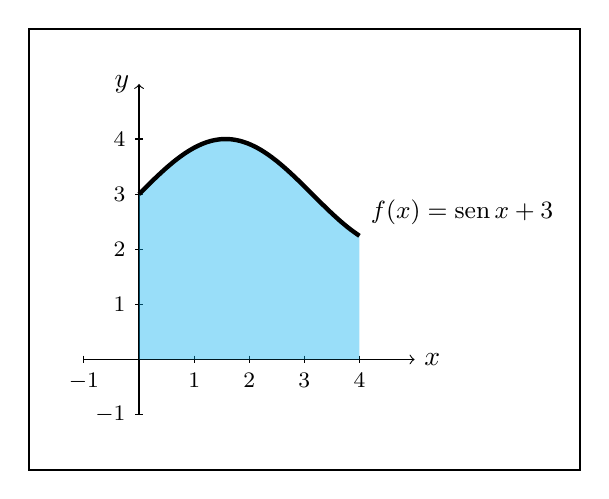
\begin{tikzpicture}[scale=0.7]
			\draw[thick] (-2,-2) rectangle (8, 6);
			% Eixos
			\draw[->] (-1,0) -- (5,0) node[right] {$x$};
			\draw[->] (0,-1) -- (0, 5) node[left] {$y$};
			% Rótulos
			\foreach \i in {-1,1,2,3,4}{
				\draw (\i,2pt)--(\i, -2pt) node[below]{{\footnotesize $\i$}};
			}
			
			\foreach \i in {-1,1,2,3,4}{
				\draw (2pt,\i)--(-2pt, \i) node[left]{{\footnotesize $\i$}};
			}
			\fill[domain=0:4,smooth,variable=\x, cyan, fill opacity=0.4]  plot ({\x},{3+sin(\x r)})--(4,0)--(0,0);
			% Yes, this is drawn twice, but I wanted the shading to match the over/under pictures following.
			
			
			\draw[domain=0:4,smooth,variable=\x, ultra thick]  plot ({\x},{3+sin(\x r)})  node[above right] {{\small $f(x) = \textrm{sen}\,x + 3$}};
		\end{tikzpicture}
		
	}{
		\Fonte{Elaborado pelo autor}
	}   
\end{figure}

Agora, tomemos como exemplo a função $f(x) = x^2$, mas não invés de particionarmos o domínio da função, a função simples é construída conforme uma partição feita na imagem.
Assim, tomemos uma função $\phi_1$ pondo 
$$
\phi_1(x) =\left\{
\begin{array}{ll}
	0, & \textrm{se\ } 0 \leq f(x) < 2^{-1} \\
	2^{-1}, & \textrm{se\ } 2^{-1} \leq f(x) < 2\cdot2^{-1} \\
	1, & \textrm{se\ } f(x) \geq 1
\end{array}
\right.
$$
Note que a função $\phi_1$ é simples, mas seus valores são escolhidos por meio da partição da imagem conforme explicitado na imagem da figura \ref{fig: Lebesgue gráfico da função phi 1}.
\begin{figure}[h!]
	\centering
	\Caption{\label{fig: Lebesgue gráfico da função phi 1}Gráfico da função $\phi_1$} 
	\UECEfig{}{
		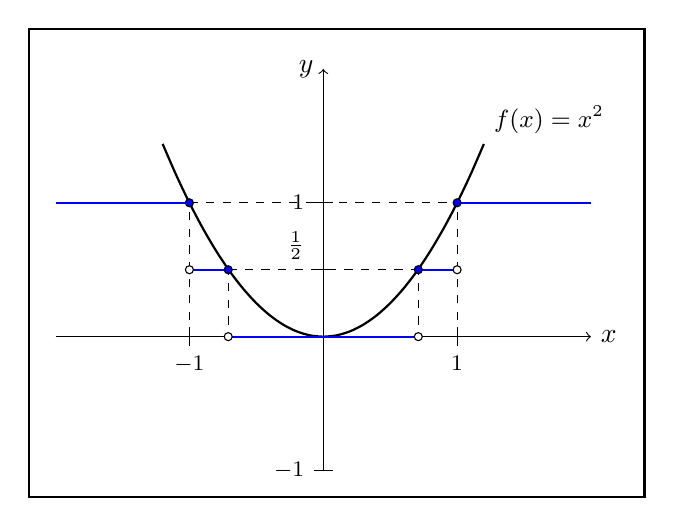
\begin{tikzpicture}[scale=1.7]
			\draw[thick] (-2.2,-1.2) rectangle (2.4, 2.3);
			% Eixos
			\draw[->] (-2,0) -- (2,0) node[right] {$x$};
			\draw[->] (0,-1) -- (0, 2) node[left] {$y$};
			% Rótulos
			\foreach \i in {-1,1}{
				\draw (\i,2pt)--(\i, -2pt) node[below]{{\footnotesize $\i$}};
			}
			
			\foreach \i in {-1, 1}{
				\draw (2pt,\i)--(-2pt, \i) node[left]{{\footnotesize $\i$}};
			}
			
			\draw (2pt,0.5)--(-2pt, 0.5) node[above left]{\footnotesize $\frac{1}{2}$};
			
			%\fill[domain=-1:1,smooth,variable=\x, cyan, fill opacity=0.4]  plot ({\x},{\x*\x})--(4,0)--(0,0);
			% Yes, this is drawn twice, but I wanted the shading to match the over/under pictures following.
			
			
			\draw[domain=-1.2:1.2,smooth,variable=\x, thick]  plot ({\x},{\x*\x})  node[above right] {{\small $f(x) = x^2$}};
			
			
			% Função $\phi_1$
			\draw[domain=-0.71:0.71,smooth,variable=\x,thick, blue]  plot ({\x},{0});
			
			\draw[domain=-1:-0.71,smooth,variable=\x,thick, blue]  plot ({\x},{0.5});
			\draw[domain=0.71:1,smooth,variable=\x,thick, blue]  plot ({\x},{0.5});
			
			\draw[domain=-2:-1,smooth,variable=\x,thick, blue]  plot ({\x},{1});
			\draw[domain=1:2,smooth,variable=\x,thick, blue]  plot ({\x},{1});
			
			% Retas auxiliares
			\draw[dashed] (-0.71,0.09) -- (-0.71,0.5);
			\draw[dashed] (0.71,0.09) -- (0.71,0.5);
			
			\draw[dashed] (-0.71,0.5) -- (0.71,0.5);
			
			\draw[dashed] (-1,1) -- (1,1);
			
			\draw[dashed] (-1,0) -- (-1,1);
			\draw[dashed] (1,0) -- (1,1);
			
			% Bolinhas
			\draw[fill=white] (-0.71,0) circle (0.03);
			\draw[fill=white] (0.71,0) circle (0.03);
			
			\draw[fill=blue] (-0.71,0.5) circle (0.03);
			\draw[fill=blue] (0.71,0.5) circle (0.03);
			
			\draw[fill=white] (-1,0.5) circle (0.03);
			\draw[fill=white] (1,0.5) circle (0.03);
			
			\draw[fill=blue] (-1,1) circle (0.03);
			\draw[fill=blue] (1,1) circle (0.03);
			
		\end{tikzpicture}
		
	}{
		\Fonte{Elaborado pelo autor}
	}   
\end{figure}
Vamos aproximar a função $f$ agora pela função simples $\phi_2$ construída da seguinte forma:
$$
\phi_2(x) =\left\{
\begin{array}{ll}
	0, & \textrm{se\ } 0 \leq f(x) < 2^{-2} \\
	2^{-2}, & \textrm{se\ } 2^{-2} \leq f(x) < 2\cdot2^{-2} \\
	2\cdot 2^{-2}, & \textrm{se\ } 2\cdot 2^{-2} \leq f(x) < 3\cdot2^{-2}\\
	3\cdot 2^{-2}, & \textrm{se\ } 3\cdot 2^{-2} \leq f(x) < 4\cdot2^{-2}\\
	4\cdot 2^{-2}, & \textrm{se\ } 4\cdot 2^{-2} \leq f(x) < 5\cdot2^{-2}\\
	5\cdot 2^{-2}, & \textrm{se\ } 5\cdot 2^{-2} \leq f(x) < 6\cdot2^{-2}\\
	6\cdot 2^{-2}, & \textrm{se\ } 6\cdot 2^{-2} \leq f(x) < 7\cdot2^{-2}\\
	7\cdot 2^{-2}, & \textrm{se\ } 7\cdot 2^{-2} \leq f(x) < 8\cdot2^{-2}\\
	2, & \textrm{se\ } f(x) \geq 2\\
\end{array}
\right.
$$
Assim, na figura \ref{fig: Lebesgue gráfico da função phi 2} está a comparação com o gráfico da função $f(x) = x^2$.
\begin{figure}[h!]
	\centering
	\Caption{\label{fig: Lebesgue gráfico da função phi 2}Gráfico da função $\phi_2$} 
	\UECEfig{}{
		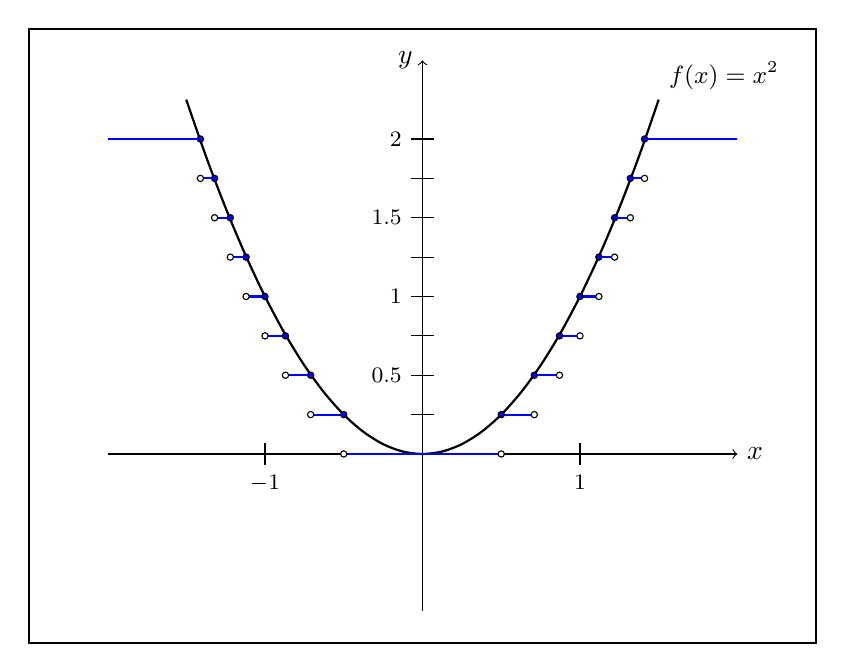
\begin{tikzpicture}[scale=2]
			\draw[thick] (-2.5,-1.2) rectangle (2.5, 2.7);
			% Eixos
			\draw[->] (-2,0) -- (2,0) node[right] {$x$};
			\draw[->] (0,-1) -- (0, 2.5) node[left] {$y$};
			% Rótulos
			\foreach \i in {-1,1}{
				\draw (\i,2pt)--(\i, -2pt) node[below]{{\footnotesize $\i$}};
			}
			
			\foreach \i in {0.5, 1, 1.5, 2}{
				\draw (2pt,\i)--(-2pt, \i) node[left]{{\footnotesize $\i$}};
			}
			
			\foreach \i in {0.25, 0.75, 1.25, 1.75}{
				\draw (2pt,\i)--(-2pt, \i);
			}
		%	\draw (2pt,0.5)--(-2pt, 0.5) node[above left]{\footnotesize $\frac{1}{2}$};
			
			%\fill[domain=-1:1,smooth,variable=\x, cyan, fill opacity=0.4]  plot ({\x},{\x*\x})--(4,0)--(0,0);
			% Yes, this is drawn twice, but I wanted the shading to match the over/under pictures following.
			
			
			\draw[domain=-1.5:1.5,smooth,variable=\x, thick]  plot ({\x},{\x*\x})  node[above right] {{\small $f(x) = x^2$}};
			
			
			% Função $\phi_2$
			\draw[domain=-0.5:0.5,smooth,variable=\x,thick, blue]  plot ({\x},{0});
			
		
			\draw[domain=-0.71:-0.5,smooth,variable=\x,thick, blue]  plot ({\x},{0.25});
			\draw[domain=0.5:0.71,smooth,variable=\x,thick, blue]  plot ({\x},{0.25});
			
			\draw[domain=-0.87:-0.71,smooth,variable=\x,thick, blue]  plot ({\x},{0.5});
			\draw[domain=0.71:0.87,smooth,variable=\x,thick, blue]  plot ({\x},{0.5});
			
			\draw[domain=-1:-0.87,smooth,variable=\x,thick, blue]  plot ({\x},{0.75});
			\draw[domain=0.87:1,smooth,variable=\x,thick, blue]  plot ({\x},{0.75});
						
			\draw[domain=-1.12:-1,smooth,variable=\x,thick, blue]  plot ({\x},{1});
			\draw[domain=1:1.12,smooth,variable=\x,thick, blue]  plot ({\x},{1});
			
			\draw[domain=-1.22:-1.12,smooth,variable=\x,thick, blue]  plot ({\x},{1.25});
			\draw[domain=1.12:1.22,smooth,variable=\x,thick, blue]  plot ({\x},{1.25});
			
			\draw[domain=-1.32:-1.22,smooth,variable=\x,thick, blue]  plot ({\x},{1.5});
			\draw[domain=1.22:1.32,smooth,variable=\x,thick, blue]  plot ({\x},{1.5});
			
			
			\draw[domain=-1.41:-1.32,thick,variable=\x,thick, blue]  plot ({\x},{1.75});
			\draw[domain=1.32:1.41,thick,variable=\x,thick, blue]  plot ({\x},{1.75});
			
			\draw[domain=-2:-1.41,thick,variable=\x,thick, blue]  plot ({\x},{2});
			\draw[domain=1.41:2,thick,variable=\x,thick, blue]  plot ({\x},{2});
			
			% Bolinhas
			\draw[fill=white] (-0.5,0) circle (0.02);
			\draw[fill=white] (0.5,0) circle (0.02);
			
			\draw[fill=blue] (-0.5, 0.25) circle (0.02);
			\draw[fill=blue] (0.5, 0.25) circle (0.02);
			
			\draw[fill=white] (-0.71,0.25) circle (0.02);
			\draw[fill=white] (0.71,0.25) circle (0.02);
			
			\draw[fill=blue] (-0.71,0.5) circle (0.02);
			\draw[fill=blue] (0.71,0.5) circle (0.02);
			
			\draw[fill=white] (-0.87,0.5) circle (0.02);
			\draw[fill=white] (0.87,0.5) circle (0.02);
			
			\draw[fill=blue] (-0.87,0.75) circle (0.02);
			\draw[fill=blue] (0.87,0.75) circle (0.02);
			
			\draw[fill=white] (-1,0.75) circle (0.02);
			\draw[fill=white] (1,0.75) circle (0.02);
			
			\draw[fill=blue] (-1,1) circle (0.02);
			\draw[fill=blue] (1,1) circle (0.02);
			
			\draw[fill=white] (-1.12,1) circle (0.02);
			\draw[fill=white] (1.12,1) circle (0.02);
			
			\draw[fill=blue] (-1.12,1.25) circle (0.02);
			\draw[fill=blue] (1.12,1.25) circle (0.02);
			
			\draw[fill=white] (-1.22,1.25) circle (0.02);
			\draw[fill=white] (1.22, 1.25) circle (0.02);
			
			\draw[fill=blue] (-1.22,1.5) circle (0.02);
			\draw[fill=blue] (1.22, 1.5) circle (0.02);
			
			\draw[fill=white] (-1.32,1.5) circle (0.02);
			\draw[fill=white] (1.32, 1.5) circle (0.02);
			
			\draw[fill=blue] (-1.32,1.75) circle (0.02);
			\draw[fill=blue] (1.32, 1.75) circle (0.02);
			
			\draw[fill=white] (-1.41,1.75) circle (0.02);
			\draw[fill=white] (1.41, 1.75) circle (0.02);
			
			\draw[fill=blue] (-1.41,2) circle (0.02);
			\draw[fill=blue] (1.41, 2) circle (0.02);
		\end{tikzpicture}
		
	}{
		\Fonte{Elaborado pelo autor}
	}   
\end{figure}

Dito isto, adiante formalizaremos que dada uma função $f \in \menfus$, então ela pode ser aproximada por uma sequência de funções simples conforme o teorema adiante.

\begin{env}{Teorema}\textbf{(Aproximação Via Funções Simples)}
	\label{teo:aproximação via funções simples}
	Se $f$ é uma função não negativa em $\menfus$, então existe uma sequência de funções $(\varphi_n)$ tal que $\phi \in \menfus, \forall \ n \in \N$ de forma que
	\begin{enumerate}[label*=(\roman*)]
		\item Cada $\varphi_n$ é uma função simples, isto é, possui apenas uma quantidade finita de valores reais;
		\item $0 \leq \varphi_n(x) \leq f(x)$ para todo $x \in X$ e $n \in \N$;
		\item $\displaystyle\lim_{n \to \infty} \varphi_n(x) = f(x)$ para todo $x \in X$.
	\end{enumerate}
\end{env} 

\begin{prova}
	Vamos mostrar a existência das sequência por construção.
	Essa construção será realizada por meio de partições da imagem da seguinte maneira:
	
	$$
	\varphi_n(x) =\left\{
	\begin{array}{ll}
		0, & \textrm{se\ } 0 \leq f(x) < 2^{-n} \\
		2^{-n}, & \textrm{se\ } 2^{-n} \leq f(x) < 2\cdot2^{-n} \\
		2\cdot2^{-n}, & \textrm{se\ } 2\cdot2^{-n} \leq f(x) < 3\cdot2^{-n} \\
		\vdots & \vdots \\
		k\cdot2^{-n}, & \textrm{se\ } k\cdot2^{-n} \leq f(x) < (k+1)\cdot2^{-n} \\
		\vdots & \vdots \\
		n, & \textrm{se\ } f(x) \geq n
	\end{array}
	\right.
	$$
	Simplificadamente podemos escrever
	$$
	\varphi_n(x) =\left\{
	\begin{array}{ll}
		k\cdot2^{-n}, & \textrm{se\ } k\cdot2^{-n} \leq f(x) < (k+1)\cdot2^{-n}, \textrm{para } k = 0,1,2, \ldots, n2^n-1 \\
		n, & \textrm{se\ } f(x) \geq n
	\end{array}
	\right.
	$$
	Com isso, podemos ver que $\varphi_n$ é uma função simples e que $0\leq \varphi_n(x)\leq f(x)$. Além disso, $\varphi_n$ é uma mensurável para todo $n \in \N$, pois trata-se de uma sequência de um funções simples.
	Observe que dado $n \in \N$ temos que
	$\phi_n(x) = k2^{-n}$ desde que 
	$k2^{-n} \leq f(x) < (k+1)2^{-n}$.
	Como  $k2^{-n}+2^{-n}$, percebemos que
	\begin{align*}
		k2^{-n} \leq f(x) < (k+1)2^{-n}
		\Rightarrow &
		\ k2^{-n} \leq f(x) < k2^{-n} + 2^{-n}\\
		\Rightarrow &
		\ \phi_n(x) \leq f(x) < \phi_n(x) + 2^{-n}\\
		\Rightarrow &
		\ \phi_n(x) - 2^{-n} \leq f(x) < \phi_n(x) + 2^{-n}\\
		\Rightarrow &
		\ |f(x) - \phi_n(x)| <  2^{-n}.		
	\end{align*}
	Como 
	$\dlim_{n \to +\infty} 2^{-n} = 0$.
	Segue que
	$\dlim_{n \to +\infty} \phi_n(x) = f(x)$.
\end{prova}

Esse teorema nos mostra que dada qualquer função não negativa mensurável, podemos aproximar seus valores por funções simples de maneira que o limite dessa sequência de funções simples convergem para a função que tomamos inicialmente.
Diante disso, nada mais natural que definir a integral de Lebesgue para funções não negativas quaisquer da maneira que segue
\begin{env}{Definição}
	\label{def:integral de uma função qualquer não negativa}
	Se $f \in M^+(X,\cc)$, nós definimos a integral de $f$ com respeito à medida $\mu$, sendo o valor real estendido
	$$
	\int f d\mu = sup \int \varphi d\mu
	$$
	Onde o supremo é sobre todas as funções simples $\varphi \in \menfus$ tal que  $0 \leq \varphi \leq f(x)$ para todo $x \in X$
	\cite{bartle}. 
\end{env}
\begin{env}{Definição}
	\label{def: integral de uma função não neg com respeito a um conjunto específico}
	Se $f \in \menfus$ e $E \in \cc$, então $f\chi_{E} \in \menfus$, definimos a integral de $f$ sobre o conjunto $E$ com respeito à medida $\mu$ como sendo o número real estendido
	$$
	\displaystyle \int_E f d\mu = \int f\chi_E d\mu.
	$$
\end{env}

Agora desejamos realizar operações aritméticas com essa expansão da definição, conforme fizemos para a integral de funções simples.
Para tal, precisamos mostrar a monoticidade da integral de funções não negativas tanto à respeito de uma outra função integral quanto à um conjunto.
Isso faremos por meio dos lemas a seguir

\begin{env}{Lema}
	\label{lem:monoticiadade da integral de funções não negativas}
	Se $f$ e $g$ são elementos de $M^+(X,\cc)$ com $f \leq g$, então 
	$ \displaystyle
	\displaystyle\int fd\mu \leq \int g d\mu.
	$
\end{env}
\begin{prova}
	Suponha que $\int f d\mu = \sup \varphi d\mu$ e $\int g d\mu = \sup \psi d\mu$ onde $\psi, \varphi$ são funções simples não negativas tais que
	$ \varphi \leq f$ e $\psi \leq g$.
	Sejam $A$ e $B$ os conjuntos das integrais de todas as funções simples que satisfazem $ 0\leq \varphi \leq f$ e $0\leq \psi \leq g$, respectivamente.
	Isto é, 
	$$
	A =\left\{
	\dsum_{j =1}^n a_j \mu(E_j); \ \phi = \dsum_{j =1}^n a_j\chi_{E_j}\ \textrm{e}\  0 \leq \varphi(x) \leq f(x)
	\right\}
	$$
	e
	$$
	B =\left\{
	\dsum_{k =1}^m b_k \mu(F_k); \ \phi = \dsum_{k =1}^m b_k\chi_{F_k}\ \textrm{e}\  0 \leq \psi(x) \leq g(x)
	\right\}
	$$
	Por hipótese, $ f\leq g$. 
	Logo, $0 \leq \varphi(x) \leq f(x) \leq g(x)$ para todo $x \in X$ acarretando que $A \subset B$.
	Desta forma, $\displaystyle\sup_A \dsum_{j =1}^n a_j \mu(E_j) \leq \sup_B \dsum_{k =1}^m b_k \mu(F_k)$.
	Portanto, $\displaystyle\int f d\mu \leq \int g d\mu$.
	
\end{prova}
\begin{env}{Lema}
	\label{lem:monoticiadade da integral com conjunto em funções não negativas}
	Se $f$ é um elemento de $M^+(X,\cc)$ e $E,F \in \cc$ com $E \subseteq F$, então 
	$$
	\int_E fd\mu \leq \int_F f d\mu.
	$$
	\vspace{-0.2cm}
\end{env}
\begin{prova}
	Como $E \subseteq F$, então $\chi_E \leq \chi_F$.
	Assim, $f\chi_E \leq f\chi_F$.
	Segue, pelo lema anterior que, 
	$$
	\int_E f d\mu 
	=
	\int f\chi_E d\mu
	\leq 
	\int f\chi_F d\mu
	=
	\int_F f d\mu.
	$$
	Portanto, $ \displaystyle 
	\int_E f d\mu 
	\leq 
	\int_F f d\mu.
	$
\end{prova}

\begin{env}{Teorema}\textbf{(Teorema da Convergência Monótona)}
	\label{teo:Convergencia Monótona}
	Se $(f_n)$ é uma sequência monótona crescente de funções mensuráveis, não negativas, que converge para uma função $f$, então
	$ \displaystyle
	\int f d\mu = \dlim_{n \to \infty} \int f_n d\mu
	$
\end{env}
\begin{prova}
	Pelo \ref{cor:convergencia-de-uma-sequencia-mensuravel}, se temos uma sequência de funções mensuráveis que converge para uma função $f$, então $f$ também é mensurável.
	Além disso,
	como $(f_n)$ é crescente, então $f_n \leq f\ \forall n \in \N$.
	Seque, pelo \ref{lem:monoticiadade da integral de funções não negativas} que 
	$ \displaystyle
	\int f_n\ d\mu \leq \int f\ d\mu
	$
	Para todo $n \in \N$.
	Desta maneira, 
	$$
	\dlim_{n \to +\infty}\int f_n d\mu \leq \int f d\mu.
	$$
	Por outro lado, sejam $\alpha \in \R$ tal que $0 < \alpha <1$ e 
	$\varphi$ uma função simples mensurável tal que $0 \leq \varphi \leq f$.
	Tomando $n \in \N$ tais que $f_n(x) \geq \alpha \varphi(x)$, construa
	os conjuntos 
	$$
	A_n =\{x \in X ;\ f_n(x) \geq \alpha \varphi(x)\}.
	$$
	Com isso, podemos observar que cada $A_n \subset X$, $A_{n} \subseteq A_{n+1}$
	e que $X = \displaystyle \bigcup_{n \in \N}A_n$.
	Desta maneira, usando o  \ref{lem:monoticiadade da integral com conjunto em funções não negativas} e \ref{lem:monoticiadade da integral de funções não negativas} temos que 
	\begin{equation}
		\label{eq:desigualdade da volta}
		\int_{A_n} \alpha\varphi d\mu
		\leq
		\int_{A_n} f_n d\mu
		\leq
		\int f_n d\mu.		
	\end{equation}
	Como $(A_n)$ é uma sequência monótona crescente que a união é igual ao conjunto $X$, observamos que, pela  \ref{prop:limite-sequencia-crescente} que para uma medida $\mu$ vale
	$$
	\mu(X) = \mu\left(\bigcup_{n \in \N}A_n\right) = \lim_{n \to +\infty} \mu(A_n)
	$$
	Só que pelo  \ref{teo:medida-atraves-de-uma-integral} $\int \varphi \chi_E d\mu$ é uma medida.
	Desta forma, 
	$$
	\dlim_{n \to +\infty} \int_{A_n} \varphi d\mu 
	= \dlim_{n \to +\infty} \int \varphi \chi_{A_n} d\mu
	= \int \varphi \chi_X d\mu
	= \int \varphi d\mu.
	$$
	Substituindo isso na equação \ref{eq:desigualdade da volta} obtemos
	$$
	\alpha \int \varphi d\mu \leq \dlim_{n \to +\infty} \int f_n d\mu.
	$$
	Como $\alpha \in (0,1)$ segue que
	$$
	\int \varphi d\mu \leq \dlim_{n \to +\infty} \int f_n d\mu.
	$$
	Finalmente, por $\varphi$ ser uma função não negativa simples arbitrária que satisfaz $0\leq \varphi \leq f$, obtemos
	$$
	\int f d\mu 
	= \sup_{\varphi} \int \varphi d\mu \leq \dlim_{n \to +\infty}\int f_n d\mu.
	$$
	Disso tudo,
	$$
	\int f d\mu 
	\leq 
	\dlim_{n \to +\infty}\int f_n d\mu
	\leq
	\int f d\mu.
	$$
	Portanto,  $\displaystyle \dlim_{n \to +\infty}\int f_n d\mu
	=
	\int f d\mu$ como desejávamos.
\end{prova}

O teorema anterior nos permite mostrar as operações aritméticas para integral de Lebesgue para funções não negativas quaisquer como apresentaremos adiante.

\begin{env}{Corolário}
	Se $f \in M^+(X, \cc)$ e $c \geq 0$, então $cf \in M^+(X, \cc)$ e vale
	$ \displaystyle
	\int cf d\mu = c\int f d\mu.
	$
\end{env}


\begin{prova}
	Se o número real for zero, então o resultado sai de forma imediata.
	Suponha que $c > 0$. 
	Assim, pelo  \ref{teo:aproximação via funções simples}, existe uma sequência de funções simples $\varphi_n \in M^+$ para todo $n \in \N$ que converge para a função $f$.
	Logo, a sequência $(c\varphi_n)$ converge para $cf$.
	Desta forma, ao aplicarmos o \ref{teo:aritmetica-com-integrais-de-funções-simples} e o
	\ref{teo:Convergencia Monótona}, obtemos
	$$
	\int c f d\mu 
	= \dlim_{n \to +\infty} \int c\varphi_n d\mu 
	= \dlim_{n \to +\infty}\left( c\cdot \int \varphi_n d\mu\right)
	= c\cdot \left(\dlim_{n \to +\infty} \int \varphi_n d\mu\right)
	= c \int f d\mu.
	$$
	Como queríamos demonstrar.
\end{prova}

\begin{env}{Corolário}
	\label{cor:soma de integrais de funções não negativas}
	Se $f$ e $g$ são funções não negativas e $\cc$-mensuráveis, então  a soma $f + g$ também é uma função $\cc$-mensurável e vale
	$ \displaystyle
	\int (f + g) d\mu = \int f d\mu + \int g d\mu
	$ \cite{bartle}. 	
\end{env}
\begin{prova}
	Analogamente ao corolário anterior, tomemos duas sequências de funções simples $(\varphi_n)$ e $(\psi_n)$ ambas monótonas e crescentes tal que convergem, respectivamente, para $f$ e $g$.
	Segue, pelo  \ref{teo:aritmetica-com-integrais-de-funções-simples} e o
	\ref{teo:Convergencia Monótona} que
	$$
	\int(f+ g) d\mu
	= \dlim_{n \to +\infty} \int (\varphi_n +\psi_n) d\mu
	= \dlim_{n \to +\infty}\int \varphi_nd\mu + \dlim_{n \to +\infty} \int \psi_n d\mu
	= \int f d\mu + \int g d\mu.
	$$
\end{prova}

Note que os resultados tratam apenas de funções monótonas e nem sempre teremos essa condição \enquote{perfeita} para nossas sequências.
Assim, o próximo resultado nos apresenta uma maneira de trabalhar com sequências que não são monótonas.

\begin{env}{Teorema}\textbf{(Lema de Fatou)}
	\label{teo:lema de fatou}
	Se $(f_n)$ é uma sequência tal que $f_n \in M^+(X, \cc)$ para qualquer que seja $n \in \N$, então 
	$\displaystyle
	\int(\lim \inf f_n)d\mu \leq \lim \inf \int f_n d\mu$ \cite{bartle}. 
\end{env}
\begin{prova}
	Tome a sequência $g_m = \displaystyle \inf_{n \in \N}\{f_m, f_{m+1},...\}$.
	Assim, enquanto $m\leq n$ nós temos $g_m \leq f_n$.
	Neste caso,
	$$
	\int g_m d\mu \leq \int f_n d\mu.
	$$
	Como $(g_m)$ é crescente e converge para $\lim\inf f_n$, nós temos que 
	$$
	\int g_m d\mu \leq \lim \inf \int f_n d\mu.
	$$
	Logo, pelo Teorema da Convergência Uniforme,
	$$
	\int (\lim \inf f_n)d\mu = \lim \int g_m d\mu \leq \lim \inf \int f_n d\mu.
	$$ 
\end{prova}
 % Discurssão sobre a integral de Rienmann
  
\begin{env}{Corolário}
	Se $f \in M^+(X, \cc)$ e $\lambda$ é definida sobre $\cc$ pondo
	$
	\displaystyle\lambda(E) = \int_E fd\mu 
	$,
	então $\lambda$ é uma medida.
\end{env}

\begin{prova}
	Uma vez que $f \geq 0$, obtemos que $\lambda(E) \geq 0$, por definição.
	Caso $E = \varnothing$, então $f\chi_E \equiv 0$ acarretando que $\lambda(\varnothing) = 0$.
	Por fim, tome $(E_n)$ uma sequência disjunta do conjunto $\cc$ e defina
	$f_n$ pondo
	$$
	f_n = \sum_{k =1}^nf\chi_{E_k}
	$$
	Segue do \ref{cor:soma de integrais de funções não negativas} que
	$$
	\int f_n d\mu
	= \int \left(\sum_{k =1}^nf\chi_{E_k}\right) d\mu
	= \sum_{k =1}^n \left(\int f\chi_{E_k}\right) d\mu
	= \sum_{k =1}^n \left(\int_{E_k} f\right) d\mu
	= \sum_{k =1}^n \lambda(E_k)
	$$
\end{prova}

%%%%%%%%% Definir QUASE TODO PONTO



\begin{env}{Corolário}
	Suponha que $f \in M^+(X, \cc)$. Então
	$f(x) = 0$ em quase todo ponto de $X$ se, e somente se $\displaystyle \int fd\mu = 0$.
\end{env}

\begin{prova}
	Suponha $f(x) = 0$ $\mu$-q.t.p.
	Assim, se $E = \{ x \in X: f(x) > 0\}$, então $\mu(E) = 0$.
	Tome a sequência $f_n = n\chi_E$.
	Dessa forma $\displaystyle f \leq \lim \inf_{n \in \N} f_n$.
	Segue, pelo Lema de Fatou que
	$$
	0 
	\leq
	\int f d\mu
	\leq
	\int (\lim \inf f_n) d\mu
	\leq
	\lim \inf \int f_n d\mu
	=
	0.
	$$
	Ou seja, $\displaystyle\int f d\mu = 0$.
	Reciprocamente, suponha que $\displaystyle\int f d\mu = 0$.
	Tome uma sequência de conjuntos 
	$E_n = \left\{ x \in X. f(x) > \dfrac{1}{n}\right\}$ tal que 
	$f \geq \left(\dfrac{1}{n}\right)\chi_{E_n}$.
	Assim, $\int f d\mu \geq \int \left(\dfrac{1}{n}\right)\chi_{E_n} d\mu$.
	Só que 
	$\int \left(\dfrac{1}{n}\right)\chi_{E_n} d\mu
	= \dfrac{1}{n}\mu(E_n) \geq 0.
	$
	Segue que
	$$
	0 = \int f d\mu 
	\geq 
	\dfrac{1}{n}\mu(E_n) \geq 0
	$$
	Ou seja $\mu(E_n) = 0$ para todo $n \in \N$.
	Assim, todo $E_n$ tem medida nula.
	Segue, pela \ref{prop:medida-nula-união}
	que o conjunto $\{x \in X; f(x) > 0\}$ tem medida nula, pois
	$\{x \in X; f(x) > 0\}
	=
	\displaystyle
	\bigcup_{n \in \N} E_n.
	$
	
\end{prova}
Finalizaremos esta subseção apresentando um corolário do Teorema da Convergência Monótona que enfatiza claramente a diferença entre a Integral de Riemann e a Integral de Lebesgue.

\begin{env}{Corolário}
	\label{contraexemplo}
	Se $(g_n)$ é uma sequência de funções em $M^+(X, \cc)$, então 
	$$
	\int \left(\dsum_{n = 1} ^\infty g_n\right)d\mu
	=
	\dsum_{n = 1} ^\infty \left(\int g_n d\mu\right).
	$$
\end{env}
\begin{prova}
	O resultado sai imediatamente da aplicação do Teorema da Convergência Monótona considerando a sequência de funções $f_n \in M^+(X, \cc)\ \forall\  n \in \N$ tais que
	$f_n = g_1 + \cdots + g_n  $.
\end{prova}

Pode ser que, até agora, tudo que definimos e discorremos não apresente diferença relevante da teoria da Integral de Riemann, a menos de sua construção.
Para que não haja dúvidas que a teoria da integração de Lebesgue generaliza a teoria da integração Riemann, vamos mostrar um contraexemplo do \ref{contraexemplo} para a integral de Riemann. 
Seja $C = \Q \cap [0,1]$ e defina a sequência de funções $f_n: [0,1] \to \R$ definida por $f_n(x) = \chi_C$ para todo $n \in \N$.
Desta forma, como $C$ é enumerável, segue que $\displaystyle \int_{0}^{1} f_n(x)dx = \int_{0}^{1} \chi_C(x) dx = 0$
\footnote{Isso é válido pelo seguinte teorema:
	\enquote{Para que uma função limitada $f : [a, b] \to \R$ seja
		integrável, é necessário e suficiente que o conjunto \textbf{D} dos seus
		pontos de descontinuidade tenha medida nula} \cite[p.344]{elon}.
}.
Com isso, $\dsum_{n = 1}^\infty \int_{0}^{1} f_n(x)dx = 0$.
Por outro lado, temos que
$
\dsum_{n = 1}^\infty f_n(x)
$
não é integrável segundo Rienmann.
\section{Funções Integráveis}
Definimos anteriormente apenas integrais de funções não negativas com respeito à uma medida $\mu$.
Nesta estenderemos, finalmente, este conceito para uma função qualquer de valores reais estendidos. Com isso,

\begin{env}{Definição}
	Seja $L = (X, \cc, \mu)$ a coleção de funções integráveis que consiste de todas as funções reais $\cc$-mensuráveis $f:X \to \R$ tais que as funções
	$f^+$ e $f^-$ são ambas integrais finitas com respeito à medida $\mu$.
	Neste caso, nós definimos a integral de $f$ com respeito à medida $\mu$ como
	$
	\int fd\mu
	= \int f^+ d\mu - \int f^- d\mu
	$
	Se, por ventura, $E$ for um elemento da \sigal $\cc$, então definimos
	$
	\int_E fd\mu
	= \int_E f^+ d\mu - \int_E f^- d\mu
	$ \cite{bartle}.
\end{env}

\begin{env}{Teorema}
	\label{teo:f é integrável se, só, se |f| o é}
	Uma função mensurável $f$ é um elemento de $L$ se, e somente se, $|f|$ é um elemento de $L$ \cite{bartle}.
\end{env}
\begin{prova}
	Suponha que $f \in L$.
	Por definição, isso ocorre se, e somente se, as partes positiva e negativa de $f$ são ambas elementos de $M^+$ e suas, respectivas integrais, são finitas.
	Devemos mostrar que 
	$$
		\int |f| d\mu = \int |f|^+ d\mu - \int |f|^-d\mu
	$$
	Pela \ref{def:parte-positiva e negativa}, $|f|^- = 0$, logo 
	$\int |f|^- d\mu = 0$.
	Pelo \ref{lem:f = f^+ - f^-} temos que
	$|f|^+ = |f| = f^+ + f^-$.
	Assim, $\displaystyle \int |f|^+ d\mu = \int (f^+ + f^-)d\mu$.
	Como $f^+ + f^- \in M^+(X, \cc)$, segue pelo corolário \ref{cor:soma de integrais de funções não negativas} que 
	$\displaystyle\int (f^+ + f^-)d\mu = \int f^+ d\mu + \int f^- d\mu$, ou seja $\displaystyle\int |f|^+d\mu$ é finita.
	Desta forma, 
	$$
	\int |f| d\mu 
	= \int (f^+ + f^-)d\mu - 0 
	= \int |f|^+ d\mu - \int |f|^- d\mu
	$$
	Logo, $|f| \in L$.
	A recíproca é totalmente análoga.	
\end{prova}

\begin{env}{Corolário}
	Se $|f| \in L$, então $\displaystyle \left|\int f d\mu\right| \leq \int |f| d\mu$ \cite{bartle}.
\end{env}
\begin{prova}
	Se $|f| \in L$, então $f \in L$ pelo teorema anterior.
	Logo $\int f^+ d\mu$ e $\int f^- d\mu$ são finitas e não negativas.
	Desta forma
	\begin{align*}
		\left|\int f d\mu \right|
		=
		\left|\int f^+ d\mu - \int f^- d\mu\right|
		= &
		\left|\int f^+ d\mu + \left(- \int f^- d\mu\right)\right|\\
		\leq&
		\left|\int f^+ d\mu\right| + \left|\left(- \int f^- d\mu\right)\right|\\
		=&
		\int f^+ d\mu + \int f^- d\mu\\
		= &
		\int (f^+ + f^-) d\mu\\
		=&¨
		\int |f| d\mu.
	\end{align*}
	Portanto, $\displaystyle \left|\int f d\mu \right| \leq  \int |f| d\mu.$
\end{prova}

\begin{env}{Corolário}
	\label{cor: f é mensurável, g é integrável então f é integrável}
	Se $f$ é mensurável, $g$ é integrável e temos que $|f(x)| \leq |g(x)|$ para todo $x$, então  $f$ é integrável e $\displaystyle \int |f| d\mu \leq \int |g| d\mu$ \cite{bartle}.
\end{env}
\begin{prova}
	Se $f$ é mensurável, então para uma medida $\mu$ definida sobre $(X,\cc)$, tem-se que $f \in L$. Assim, pelo teorema \ref{teo:f é integrável se, só, se |f| o é} tem-se que $|f|$ é integrável.
	Como $|f|$ e $|g|$ são função não negativas, segue pelo lema
	\ref{lem:monoticiadade da integral de funções não negativas} que 
	$\displaystyle \int |f| d\mu \leq \int |g| d\mu$.
\end{prova}


\begin{env}{Teorema}
	\label{teo: soma e multiplicação por escalar de funções integráveis}
	Se $f, g \in L$ e $\alpha \in \R$. Então
	\begin{enumerate}[label*=(\alph*)]
		\item A multiplicação por escalar $\alpha f \in L$ com $\displaystyle \int \alpha fd\mu = \alpha \int f d\mu$;
		\item A soma $(f + g) \in L$ com $\displaystyle \int (f + g) d\mu = \int f d\mu + \int g d\mu$. 
	\end{enumerate}
\end{env}
\begin{prova}
	\begin{enumerate}[label*=(\alph*)]
	\item Se $\alpha = 0$, então $\alpha f = 0$ em todo ponto de seu domínio.
	Assim,
	$
	\displaystyle\int \alpha f d\mu = 0 = \alpha \int f d\mu.
	$
	Se $\alpha > 0$, então 
	\begin{align*}
		\alpha \int f d\mu
		=&	
		\alpha \left( \int f^+ d\mu - \int f^- d\mu\right)\\
		=&
		\alpha\int f^+ d\mu - \alpha\int f^- d\mu\\
		=&
		\int\alpha f^+ d\mu - \int\alpha f^- d\mu.
	\end{align*}
	Perceba que $\alpha f^+ = (\alpha f)^+$  e $\alpha f^- = (\alpha f)^-$.
	Disso, 
	$$
	\int\alpha f^+ d\mu - \int\alpha f^- d\mu
	=
	\int(\alpha f)^+ d\mu - \int(\alpha f)^- d\mu
	=
	\int \alpha f d\mu.
	$$
	Neste caso, $\alpha f \in L$ e temos $\displaystyle \alpha \int f d\mu = \int \alpha f d\mu$. O caso $\alpha < 0$ é totalmente análogo.
	
	\item Se $f, g \in L$, então $|f|,|g| \in L$ pelo teorema \ref{teo:f é integrável se, só, se |f| o é}.
	Como $|f + g| \leq |f| + |g|$, segue que $f + g \in L$ pelo corolário \ref{cor: f é mensurável, g é integrável então f é integrável}.
	Além disso, pelo lema \ref{lem:f = f^+ - f^-}, temos 
	$f = f^+ - f^-$ e $g = g^+ - g^-$.
	Somando membro a membro, temos
	$$
	f + g = f^+ - f^-  + g^+ - g^- = f^+ + g^+ - (f^- + g^-) 
	$$
	Como $(f^+ + g^+), (f^- + g^-)$ são funções integráveis não negativas, temos que 
	$$
	\int (f + g) d\mu =  \int [f^+ + g^+ - (f^- + g^-)] d\mu 
	$$
	Pelo corolário \ref{cor:soma de integrais de funções não negativas} 
	\begin{align*}
		\int [f^+ + g^+ - (f^- + g^-)] d\mu 
		=&
		\int (f^+ + g^+)d\mu - \int(f^- + g^-) d\mu\\
		=&
		\int f^+ d\mu + \int g^+ d\mu - \int f^-d\mu - \int g^- d\mu\\
		=&
		\int f^+ d\mu - \int f^-d\mu + \int g^+ d\mu  - \int g^- d\mu\\
		=&
		\int f d\mu + \int g d\mu.
	\end{align*}
	Portanto, $\displaystyle \int (f+g)d\mu = \int f d\mu + \int g d\mu.$
	\end{enumerate}
\end{prova}

\begin{env}{Teorema}\textbf{(Teorema da Convergência Dominada de Lebesgue)}
	Seja $(f_n)$ uma sequência de funções integráveis que converge em quase todo ponto para uma uma função real mensurável $f$.
	Se existir uma função integrável $g$ tal que $|f_n| \leq g$ para todo $n \in \N$, então $f$ é integrável e $\displaystyle \int f d\mu = \dlim_{n \to +\infty} \int f_n d\mu$ \cite{bartle}.
\end{env}

\begin{prova}
	Se $(f_n)$ converge em quase todo ponto para a função $f$ e $|f_n| \leq g$ para cada $n \in \N$, então $f \leq g$ em quase todo ponto.
	Como $g$ é integrável, segue pelo \ref{cor: f é mensurável, g é integrável então f é integrável} que $f$ é integrável.
	Além disso, note que para todo $n \in \N$, temos
	$$
	|f_n| \leq g 
	\Leftrightarrow 
	f_n \leq g 
	\textrm{\ ou \ }
	 f_n \geq -g
	\Leftrightarrow
	g - f_n \geq 0
	\textrm{\ ou \ }
	g + f_n \geq 0
	$$
	Caso tenhamos $g + f_n \geq 0$ podemos utilizar o Lema de Fatou e o \ref{teo: soma e multiplicação por escalar de funções integráveis} de forma que 
	\begin{align*}
		\int g d\mu + \int f d\mu =& \int (g + f) d\mu \\
		\leq & \lim \inf \int (g + f_n) d\mu \\
		=& \lim \inf \left(\int g d\mu + \int f_n d\mu\right)\\
		=& \int g d\mu + \lim \inf \int f_n d\mu
	\end{align*}
	isso acarreta que 
	$$
	\int g d\mu + \int f d\mu \leq  \int g d\mu + \lim \inf \int f_n d\mu.
	$$
	Logo, $\displaystyle \int f d\mu \leq \lim \inf \int f_n d\mu$.
	
	Caso ocorra $g - f_n \geq 0$, aplicamos novamente o Lema de Fatou e o teorema \ref{teo: soma e multiplicação por escalar de funções integráveis}.
	Assim, 
	\begin{align*}
		\int g d\mu - \int f d\mu = \int (g - f) d\mu
		\leq  \lim \inf \int (g - f_n) d\mu
		\leq \int g d\mu + \lim \inf \int (- f_n) d\mu.
	\end{align*}
	Lembre que $\displaystyle \lim \inf \int (- f_n) d\mu = - \lim \sup \int f_n d\mu$.
	Com isso, 
	$$
	\int g d\mu - \int f d\mu \leq 
	\int g d\mu + \lim \inf \int (- f_n) d\mu
	=
	\int g d\mu - \lim \sup \int f_n d\mu.
	$$
	Desta forma, $\displaystyle \int f d\mu \geq \lim \sup \int f_n d\mu$.
	Disso tudo, observamos que 
	$$
	\lim \sup \int f_n d\mu \leq  \int f d\mu \leq \lim \inf \int f_n d\mu. 
	$$
	Portanto, $\displaystyle \lim \int f_n d\mu =  \int f d\mu $.
\end{prova}
























        
%\textbf{Objetivo Geral} \\ \\
%Conhecer aplicações da convergência de sequências de números reais no Cálculo Diferencial e Integral.  \\ % partindo de diferentes formas de demonstrações.

%\textbf{Objetivos específicos} \\ \\
%a)	Relatar algumas circunstâncias da utilização de sequências sob contextos históricos; \\ \\
%b)	Apontar teoremas que qualificam a convergência de sequências de números reais, formulando suas respectivas demonstrações; \\ \\
%c) Apresentar algumas aplicações da convergência de sequências de números reais e suas possibilidades de demonstrações no Cálculo Diferencial e Integral.


%c) Apresentar algumas possibilidades de demonstrações para casos de aplicações da convergência de sequências de números reais no Cálculo Diferencial e Integral.

\chapter{Considerações Finais}
	Neste trabalho abordamos a teoria da medida e integração, de forma simplória e resumida, tendo como pergunta diretriz de que forma pode ser apresentada a teoria da medida e integração de Lebesgue de maneira elementar para os alunos de graduação de ciências exatas?
	Com o intuito de auxiliar na obtenção da resposta, nosso objetivo geral que nos guiou em todo processo de construção do objeto de pesquisa foi: 
	conhecer algumas definições e resultados da teoria da medida e da integração de Lebesgue de forma simplificada.
	
	Desta forma, nosso primeiro objetivo específico era: definir a base do estudo da teoria da medida por meio dos espaços mensuráveis.
	Para atingir esse propósito, primeiro definimos  uma \sigal de um conjunto.
	Em seguida, denotamos que um conjunto não vazio e uma \sigal desse conjunto formam um espaço mensurável.
	Fixamos este conceito apresentando exemplos com grau crescente de abstração.
	Provamos algumas proposições sobre espaços mensuráveis e apresentamos uma \sigal especial no conjunto dos números reais, a \sigal de Borel.
	Fizemos um processo semelhante para expor as funções mensuráveis sendo os resultados focados em uma maneira mais fácil de averiguar se uma função é mensurável sem utilizar a definição diretamente.
	
	Nosso segundo objetivo específico era: conhecer a teoria da medida de maneira generalizada.
	Para obter com sucesso esse meta, precisou-se estender a reta real adicionando as noções de $-\infty$ e $+\infty$ exibindo uma álgebra específica a ser adotada.
	Com isso, na primeira parte da seção, generalizamos os resultados apresentados na seção anterior dando ênfase às mudanças que ocorreram ao mudar de $\R$ para $\overline{\R}$.
	Depois disso, definimos o que é uma medida, enunciamos e provamos propriedades sobre.
	Além disso, trouxemos vários exemplos, dentre eles, o espaço de probabilidades e a medida de um conjunto discreto.
	Todas as demonstrações tiveram o intuito de serem as mais didáticas possíveis sendo os teoremas divididos em várias proposições para que pudesse haver o melhor entendimento.
	
	Nosso último objetivo era: descrever o processo da construção da integral de Lebesgue mediante o avanço da teoria da medida.
	Para tal, desmembramos os tipos de funções para que pudesse ser um processo intuitivo da construção.
	Exibimos, inicialmente, as integrais de Lebesgue para funções simples.
	Fixamos a medida de Lebesgue para que os exemplos ficassem mais claros, pois nesta parte, a diferença entre a integral de Lebesgue e a integral de Riemann era indistinguível. 
	Ao dar continuidade, lembramos a construção da integral de Riemann para funções não negativas para que depois pudéssemos mostrar a construção de Lebesgue e evidenciar a diferença entre as duas.
	Neste momento, várias ferramentas para integrais de Lebesgue para funções não negativas foram enunciadas e provadas para que esta pudesse ser generalizada para funções quaisquer.  
   	
   	Com isso, acreditamos que a forma como foi organizado este trabalho possibilita um estudo introdutório sobre a teoria da medida e integração de Lebesgue para alunos de graduação em ciências exatas em uma disciplina optativa.
   	Essa crença surge da simplificação do texto e da teoria para que aborde coisas pontuais e não tão gerais como se é esperado em um primeiro contato com a teoria. 
   	Fazemos isso, por exemplo, quando decidimos começar diretamente com a definição de $\sigma$-álgebra ao invés de iniciar com a definição de semi-anel como faz o livro Medida e Integração de Pedro Jesus Fernandez (\citeyear{pedro}), por exemplo.
   	Além disso, tratamos primeiro de funções mensuráveis para, em seguida, trabalhamos com medida o que também não é comum na bibliografia brasileira.
   	Por fim, tentamos sempre por gráficos quando julgamos necessário o que também é escasso em livros sobre o tema por pensar em um público diferente ao que destina esse trabalho. 
   	 
    
    
    
    
    
    
    
    
    
    
    
    
    
    
    
    
    
    
        %Elementos pós-textuais	
	\bibliography{elementos-pos-textuais/referencias}
%	\imprimirapendices
		% Adicione aqui os apendices do seu trabalho
	
	%\input{elementos-pos-textuais/apendices/movimento-vizinhança-equilíbrio-estável}	
      
     \printindex

\end{document}